%\documentclass[11pt]{report}
\documentclass[12pt, twoside, ngerman]{report} 
%\documentclass[12pt,twoside]{report}
% \documentclass{article}
\usepackage{amssymb}
\usepackage{algpseudocode}
\usepackage{algorithm}
\usepackage{setspace}
\usepackage{graphicx}
\graphicspath{ {./images/} }
\usepackage{hyperref}
\usepackage{siunitx}
\usepackage{amsmath}
\usepackage{caption}
\usepackage{subcaption}
\usepackage{geometry}
\usepackage[english]{babel}
\usepackage[T1]{fontenc}
\usepackage[utf8]{inputenc}


\usepackage{tikz}
\usetikzlibrary{positioning}
% \usetikzlibrary{graphdrawing.trees}

\usepackage{booktabs}

\hypersetup{
    colorlinks=false,
    linkcolor=blue,
    filecolor=magenta,
    urlcolor=cyan,
}

% Commenting out another way to write the title.
% \title{MSc Thesis - Ranking Loss Surrogates}

\iffalse    
\author{
        Abdus Salam Khazi [
        \href{mailto:abdus.khazi@students.uni-freiburg.de}
                {Email} ]\\ \\
        \href{https://github.com/abduskhazi/ranking-loss-surrogates.git}
                {Github Repository} \cite{github_repository} \\ \\
        Supervisors:
        \begin{tabular}{ll}
             JProf. Josif Grabocka \&
			Sebastian Pineda
		\end{tabular}
       }
\fi


\begin{document}

\newgeometry{
    top=1.5in,
    bottom=1.5in,
    outer=1.75in,
    inner=1.25in,
    }

\title{
{\LARGE Master's Thesis}
\vspace{20pt}
\hrule
\vspace{20pt}
\textbf{Hyperparameter Optimization using Ranking Loss Surrogates}
\vspace{20pt}
\hrule
\vspace{20pt}
\author{{\LARGE Abdus Salam Khazi}}
\date{\LARGE \today}
\begin{figure}[h]
    \centering
    
\includegraphics[width=50mm]{images/Logo.png}
\end{figure}
\large{Albert-Ludwigs-University Freiburg
\\Representation Learning Department}
}
    
\pagenumbering{gobble}

\maketitle
    

% \date{}

\chapter*{Declaration \thispagestyle{empty}}


I hereby declare, that I am the sole author and composer of my thesis and that no other sources or learning aids, other than those listed, have been used. Furthermore, I declare that I have acknowledged the work of others by providing detailed references of said work. 

I hereby also declare, that my Thesis has not been prepared for another examination or assignment, either wholly or excerpts thereof

\vspace{100pt}

\begin{minipage}{2in}
\textbf{\underline{\hspace{100pt}}} \\
Place, Date
\end{minipage}
\hfill
\begin{minipage}{1.3in}
\textbf{\underline{\hspace{100pt}}} \\
Signature
\end{minipage}

\newpage
\pagenumbering{roman}
\begin{abstract}

Abstract goes here

\end{abstract}

\newpage

\tableofcontents
\newpage
\newpage

\pagenumbering{arabic}

\chapter{Introduction}

The performance of any machine learning model is sensitive to the hyper-parameters used during the model training. 
Instead of using a new model type, it is more helpful to tune the hyper-parameters of an existing model to improve its performance.
Learning the best hyper-parameter for an ML model is called, Hyperparameter optimization (HPO in short).

The true evaluation of a hyperparameter optimisation objective function is computationally very expensive. 
Researchers have tried to get around this problem by proposing model based HPO algorithms.
In these methods,  the true objective function is modelled by a cheap surrogate function of high representational capacity.
For example,  the Sequential Model Based Optimization (SMBO)~\cite{NIPS2011_86e8f7ab} algorithm is a very important algorithm that iterates between learning a model given a few HP configuration evaluations and using the model to propose the next candidate to evaluate.

This thesis studies various existing approaches to HPO and proposes a new idea for the same using the concept of ranking.
The proposed idea in this thesis is called \textbf{Hyperparamter Optimization using Ranking Loss Surrogates}. 
The results obtained using this model are compared against the state-of-the-art results obtained using models like FSBO,  RGPE,  TAF, and others. 

\label{ProblemOverviewlabel}
\section{Objective}
The aim is to study ranking loss surrogates in the context of Hyperparameter optimization.

\section{Overview}
This sections contains the overview of the paper and how the thesis report is organised.


\chapter{Related Work}\label{chap:relatedWork}

In this chapter,  we first define the hyper-parameter optimization problem concretely.
Then, we discuss the approaches already used to do the HP optimization.
Subsequently, we discuss some essential concepts that the thesis uses to build the proposed model.

\section{Hyper Parameter Optimization}
To find out the best hyper-parameter for any machine learning model $m$, we must first quantify a given hyper-parameter configuration $\textbf{x}$ by a real-valued number $v \in \mathbb{R}$.
If we define that
$$
\textbf{x}_1 \succ  \textbf{x}_2 \iff v_{\textbf{x}_1} < v_{\textbf{x}_2}
$$
then HPO can be defined mathematically by an abstract function, say,  $f(\textbf{x}) \mapsto \mathbb{R}$ as
$$
     \underset{\rm \textbf{x}}{\rm argmin}  f(\textbf{x}) \;\;\;  \forall \textbf{x} \in \mathbb{S}
$$
Where $\mathbb{S}$ is the hyper-parameter search space.

This function $f(\textbf{x}) \mapsto \mathbb{R}$ is evaluated in the following chronological steps:
\begin{enumerate}
\item Using a given hyper-parameter configuration $\textbf{x}$,  we train our model $m$ to obtain the model $m^{trained}_\textbf{x}$. It consists of learning the parameters of our model, E.g., learning the weights and biases of a Deep Neural Network.
We use the training data to learn this model.
\item The validation data is passed through $m^{trained}_\textbf{x}$ to obtain the required results.
These results are evaluated based on an evaluation criterion '$\textrm{eval}$'. This criterion is different for different problems, e.g., Regression and Classification.
The result of this evaluation is a real-value that gives a score for the configuration $\textbf{x}$.
\end{enumerate}

Hence the function $f(\textbf{x}) \mapsto \mathbb{R}$ can be written as 
$$
f(m^{trained}_\textbf{x} (\textrm{Data}_\textrm{val})) \mapsto \mathbb{R}
$$

Finally, the HPO problem can be defined using the following equation:
\begin{equation}\label{eq:hpoobjectivefunc}
\underset{\rm \textbf{x}}{\rm argmin} \;\; f(m^{trained}_\textbf{x} (\textrm{Data}_\textrm{val})) \mapsto \mathbb{R}   \;\;\;  \forall \textbf{x} \in \mathbb{S}
\end{equation}

One way to view this objective function non-mathematically is that we are trying to select a hyper parameter setting of the given model to obtain the best (lowest) validation error~\cite{fsbopaper}.

\subsubsection{HPO Constraints}\label{sec:hpoConstraints}

Hyperparameter optimization is different from other optimization methods because it has different constraints~\cite{bayesianOptimizationTutorial}.
It is because of the peculiar properties of the hyper-parameter search spaces.
Finding the correct hyper-parameter setting is generally not feasible using a brute-force approach (trying out all possible combinations of hyper-parameters) because the search space has many dimensions, and the search space may be continuous.
More specifically,  some of the important constraints of this optimization problem are:

\begin{enumerate}
\item The evaluation of a given HPO configuration is computationally expensive.
\item It is a non-convex optimization problem.
\item The process of getting $m^{trained}_\textbf{x}$ from $m$ is stochastic hence the value $v_{\textbf{x}}$ is noisy.
\item Some dimensions have conditional constraints. The values of some dimensions may depend on the values of others. For example, the number of neurons in layer three only makes sense if we have three or more layers in a neural network.
\item The search space is hybrid in terms of continuity. Some dimensions (variables) may be continuous, while others may be discrete.
Using a gradient method is hence not trivial.
\end{enumerate}

To deal with the constraints of HPO problems, researchers have used different strategies for developing HPO algorithms and models.
Some of the more prominent approaches are Black-Box HPO, 
Multi-fidelity HPO and Online HPO.

\subsection{Black-box HPO}
In this approach the HPO objective function $f$ in equation~\ref{eq:hpoobjectivefunc}
is treated as a blackbox.
The problem is generalized to finding a global optimum of $f$.
Some straightforward black-box HPO methods include Manual Search,  Grid Search, and Random Search.
The Bayesian optimization technique gives us a more sophisticated mechanism to deal with this problem. 

Manual Search in the HPO search space is feasible when we have expert knowledge of the problem and the given model. 
The idea is to select configurations step by step by observing the results obtained so we do not waste computation time evaluating similar configurations through intuition.
This approach may be helpful for small models with lesser constraints.
However, as the HPO search space becomes very large or conditional constraints become too complex, the selection of configurations becomes more and more difficult.
Hence a more systematic and automated approach is more practical.

Grid search is a more systematic approach to dividing the search space into grid points similar to those in a Euclidean graph.
Let there be $m$ dimensions in the search space $\mathbb{S}$. Let the selected number of values for each dimension be $n_1, n_2, ... n_m$. In the case of a discrete variable, the selected values will be a subset of the possible values, whereas, in the case of a continuous variable, we need to select the values based on a selected granularity.
The cross-product of the selected subsets gives us the configurations to be evaluated. Hence, the number of configurations to evaluate will be $n_1 * n_2 * ... n_m$.
The number of configurations we need to evaluate in this approach becomes a big issue for this method as the dimensions of the search spaces increase.
Hence this approach becomes intractability for large search spaces.

\begin{figure}[htb]
  \centering
    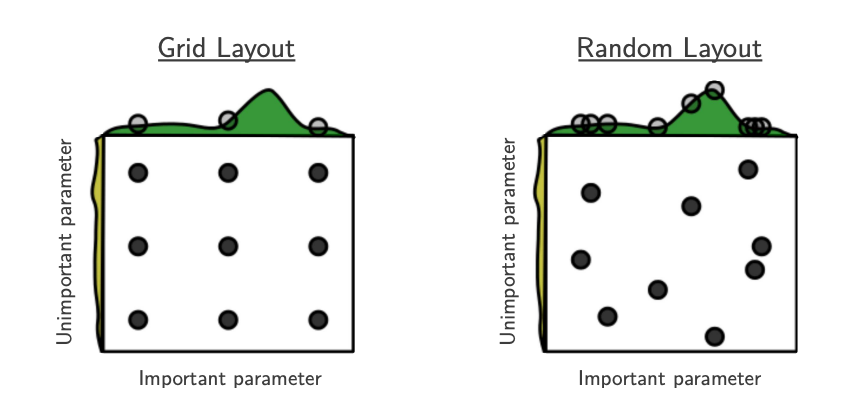
\includegraphics[scale=0.8]{images/rsgsexample}
    \caption{Illustrates Grid search and Random search in the case where 2 parameters are not equally important.  Adpated from~\cite{rshpoarticle}.}
    \label{fig:rshpofig}
\end{figure}

One issue with the Grid Search approach is that we assume that all dimensions in the HPO search space are equally important. It is not the case in many HPO problems. The Grid layout in Figure~\ref{fig:rshpofig}(left) illustrates this. For example, the learning rate in deep neural networks is much more important than many other parameters. If dimension $p$ is the most important in the search space, then it makes sense to evaluate more values of $p$. Random Search helps us solve this problem. 
The Random layout in Figure~\ref{fig:rshpofig}(right) illustrates this. 
Hence Random Search can be used as a trivial baseline for comparing other HPO models.

One advantage of these methods is that there are no restrictions on the HPO search spaces. Hence, they are suitable for any HPO problem at hand.
On the other hand, these methods are non-probabilistic.
Hence they cannot deal with noisy evaluations of the HPO configuration well.
Moreover, these methods are computationally expensive. The reason is that they do not use surrogate evaluators and train and evaluate the whole model.
Also, these search methods give us optimal HPO configurations only by chance.

\subsubsection{Bayesian Optimization}

Bayesian optimization tries to solve both computational costs and noisy evaluations of our objective function $f$.
It does this by building a model of the HPO objective function. This model is called a surrogate function.
Bayesian optimization uses known evaluations as its data to build the surrogate model. The data is of the form \{x, f(x)\} pairs.
The surrogate model is a probabilistic model. Hence, it also learns about the noise in the evaluations of the objective function.

The core procedure of the optimization process is the following:
\begin{itemize}
\item From known data $D = {(x_1, f(x_1)), (x_2, f(x_2)), (x_3, f(x_3)) .... }$, build a probabilistic model that learns the mean and variance of the objective function
\item Use the surrogate to sample the next best HPO configuration x' using a function known as acquisition function. Evaluate f(x').
\item Append (x', f(x')) to D and repeat the process.
\end{itemize}

The above process repeats till the computational resources are finished (here time), or we find an acceptable HPO configuration.
This procedure is also called SMBO (Sequential model-based Optimization).
The procedure alternates between collecting data and fitting the model with the 
collected data~\cite{SMBOPaper}.

Hence, there are two essential components of Bayesian optimization:

\begin{itemize}
\item Probabilistic surrogate model of the objective function. Some surrogates are discussed in detail in the subsequent sections in this chapter.
\item The acquisition function
\end{itemize}

\subsubsection{Acquisition functions}
The acquisition functions used in the Bayesian optimization need to balance the exploitation of information from the known/observed data points and exploration of unknown data points in the domain.
The following functions are some of the most prominent acquisition functions found in the literature~\cite{GPTutorial}
\begin{itemize}
\item \textbf{Upper Confidence Bound (UCB)}: It returns the best possible hyperparameter configuration using a linear combination of the mean and the standard deviation.
\item \textbf{Probability of Improvement}: It gives the probability that we can get a better hyperparameter configuration than the incumbent best configuration.
\item \textbf{Expected Improvement}: Given a Gaussian distribution at a new input point, it finds the expectation of improvement i.e ($f(x) - f_{max}$) over the part of normal that is greater than $f_{max}$.
\end{itemize}

 \textbf{Expected Improvement} acquisition function is used all around the thesis to make a fair comparison of the models and algorithms.


\subsection{Online HPO}
Traditionally, the objective function $f$ is fully evaluated to select a new HP configuration.
In the most general sense, this can be applied to both discrete and continuous HP search spaces.
Some advanced methods have proposed even gradient-based HP optimization.

For example,  Maclaurin et al.~\cite{hypergradient} proposed a relatively cheap method to obtain hyper gradients, i.e., gradients of hyper parameters for the whole objective function $f$.
Further,  Franceschi et al.~\cite{HPOAsBilevelOptimization} formulated the whole HPO problem as a bi level optimization problem~\cite{hutterneuripstutorial}.

In all these methods, as the hyper and model parameters are learned disjointly, they can be referred to as offline HPO.
The idea of online HPO is that it tries to evaluate and update the HP configuration during the model's training.

Sometimes only a single hyperparameter is learned online.
For example,  Baydin et al.~\cite{onlineLearningRateUpdate} propose the online learning of the learning rate. They target this hyper parameter because it is the single most important one.
In other times all parameters may be learned. Luketina et al. ~\cite{gradientbasedHPOtuning} describe this example by proposing the interleaved updating of training parameters and hyperparameters.


\subsection{Multi-fidelity HPO}
If we treat our HPO objective function $f$ as a black box function,  we would need to evaluate equation~\ref{eq:hpoobjectivefunc} fully.
This evaluation is prohibitively expensive as evaluating a single HP configuration may take days~\cite{hutter2019automated}.
Multi-fidelity hyper parameter optimization tries to solve this problem by evaluating the HP candidates on cheap functions $f_{approx}$ that approximate the objective function $f$.

Here, $f_{approx}$  is called fidelity as it reproduces the actual objective function to some degree.
For example, a fidelity could be an evaluation of the HP configuration on only a subset of data, the evaluation of the HP on downscaled image data, or learning only for a few epochs.
The idea is to trade-off between the performance of the approximate function and its optimization accuracy such that we get the best selection of HP using the least compute power.
Since we do not do the actual evaluation of HP configuration using $f$, it is an approximate optimization technique.

The technique does not belong to the black box HPO domain.
It can be understood very clearly if we consider the "few epochs" fidelity.
The optimization algorithm looks into the training process and learns the objective function to exit it earlier.
It thus gets feedback from within the "black box" of the HPO objective function.

This technique is named multi-fidelity because it may use different fidelities within the optimization process to get the best HP configuration.
While using successive having technique~\cite{successivehalving} for HPO, one can start with a given "budget fidelity," for example - a defined number of epochs or a defined amount of training time.
The budget doubles at each step of the optimization process, and we eliminate the worst-performing HP configurations for the next step.
Hence it uses "multiple" fidelities during the optimization process.


\section{Transfer-learning for HPO}

The HPO methods discussed so far evaluate each HP configuration from scratch.
In addition to being computationally inefficient,  it is contrary to how humans learn.
Humans use prior experience that they have accumulated and condition their actions on this knowledge.
Any machine learning mechanism that uses this concept is called a transfer learning method~\cite{Weiss2016}.

The concept of transfer learning can be utilized to accelerate HPO.
For example,  Gomes et al. ~\cite{svmhpmetalearnt} propose to meta-learn a set of exemplary HP configurations for the SVM.
They propose that if we learn HP configurations that previously worked well, there is a high chance of finding that a new SVM model also works with these parameters.
Reif et al.~\cite{metalearningwarmstartpaper} also proposed this concept of warm starting the HP optimization for genetic algorithms.

There are two broad ways to transfer knowledge for HP optimization: by learning surrogates or by doing warm starting of initial configurations.

\subsection{Warm starting}

Before running any HPO method, typically, experts study the data used to train the given model.
They suggest a few initial HP configurations that have worked well for similar datasets, according to their experience.
These initial configurations are evaluated for the given model, and the evaluated values act as a starting point (or hinge) for the HPO method.
The idea of warm starting is to automate the selection of the initial configurations before the HPO optimization runs.

Warm starting was used by Gomes et al. ~\cite{svmhpmetalearnt}, and Reif et al. ~\cite{metalearningwarmstartpaper}. In their respective papers, the authors used the meta-learned HP configurations as starting points for finding the optima in the HP response surface.
This idea was also proposed for the SMBO optimization algorithm by Feurer et al. ~\cite{Feurer2014UsingMT}.


\subsection{Meta-learning of surrogates}

HPO models that use surrogates like SMBO,  have an additional gateway through which previous knowledge can be injected.
The idea is to meta-learn the surrogate using previously stored meta-data from similar tasks.
This is used by Schilling et al.~\cite{Schilling2016ScalableHO} in which they learn a collection of Gaussian models for each previously similar dataset due to computational constraints.
They then use the collection of GPs as a surrogate for the SMBO procedure.
Another flavour of this approach was proposed  by Feurer et al.~\cite{Feurer2018ScalableMF} proposed the use of rank weighted GP Ensembles (RGPE) surrogates meta-learnt from previous meta data.

This meta learnt surrogate can be used in 2 different ways during the HPO optimization procedure.
For example in SMBO,  one could use it without any modification (aka fine tuning) to suggest the next best candidate to evaluate from a given HP configuration list.
On the other hand the surrogate can be further meta trained (aka fine tuned) using the available target task meta data. 

Using meta learning of surrogates,  this thesis proposes a new surrogate model.

\section{Types of Surrogates for BO in HPO}
Hyperparameter optimization using Sequential Model Based Optimization (SMBO)~\cite{NIPS2011_86e8f7ab} is a convenient method proposed in the literature.
However,  the performance of this method is heavily reliant on how well the surrogate (model in S\textbf{M}BO) models the true HPO objective.
In this section,  we discuss in details some of the powerful surrogates that may be used with SMBO.

\subsection{Gaussian Processes}

Gaussian processes~\cite{GPTutorial} are predictive machine learning models that work well with few data points (or data pairs). 
They are inherently capable of modeling uncertainty.
Hence, they are used widely in problems such as hyperparameter optimization, where uncertainty estimation is essential.
In this section, we briefly explain the Gaussian process regression intuitively.

Before we proceed,  we need to understand normal (Gaussian) distributions. 
Consider a scalar random variable $X$ that is distributed normally  (a.k.a Gaussian distribution) around a mean $\mu$ with a variance of $\sigma^2$.
The following equation defines the probability density function (PDF) of $X$: 
$$
P_X(x) = \frac{1}{\sqrt[2]{2\pi}\sigma}\exp\left(- \frac{(x - \mu)^2}{2\sigma^2}\right)
$$
Here, $X$ represents the random variable, and $x$ represents an instance of the variable~\cite{GPTutorial}.
In this case,  the mean $\mu$,  variance $\sigma^2$, and any sample $x$ are all scalars.

If the random variable $\textbf{X}$ is a vector in $\mathbb{R}^d$ where $d \in I^{+}$,  then each component of the vector can be considered as a random variable.
In this case the mean $\boldsymbol{\mu} \in \mathbb{R}^d$ whereas variance, represented by $\Sigma$, is in the $R^{d \times d}$ space.
It is because the variance of all components in any valued vector random variable $\textbf{X}$ should contain the following two types of variance
\begin{itemize}
\item Variance of a vector component w.r.t itself.
$d$ diagonal values of the matrix $\Sigma$ represent this variance.
\item Variance of each vector component w.r.t all other components. These variances are represented by the upper/lower triangular values in the matrix $\Sigma$.
\end{itemize}
The matrix $\Sigma$, also known as the Covariance matrix, thus has all values necessary to represent the variance of any vector-valued random variable.


The probability density function of a vector valued variable $\textbf{X} \in \mathbb{R}^d$ with a mean $\boldsymbol{\mu}$ and covariance matrix $\Sigma$ is given by~\cite{MITMLBook}:

$$
\mathcal{N}(\textbf{x} | \boldsymbol{\mu},  \Sigma) = 
\frac{1}{(2\pi)^{\frac{d}{2}} |\Sigma|^{\frac{d}{2}}}
\exp\left( - \frac{1}{2} (\textbf{x} - \boldsymbol{\mu})^T  \Sigma^{-1}   (\textbf{x} - \boldsymbol{\mu}) \right)
$$
This equation defines the PDF of a multivariate normal distribution.

The core idea used in the Gaussian processes is that functions can be considered as vectors of infinite dimensions.
Consider any function $f$ that has a domain $\mathbb{R}$.
If $f$ is considered to be a vector in $\mathbb{R}^{\infty}$,
then each point $i \in \mathbb{R}$  can be represented by a component $f_i$ of the function $f$.
A function,  hence,  is nothing but a sample from $\mathbb{R}^{\infty}$.
Unfortunately, functions sampled from $\mathbb{R}^{\infty}$ are too general and not useful by themselves.

The idea of Gaussian processes is to sample smooth functions from $\mathbb{R}^{\infty}$.
In any smooth function $f$, if any point $g$ is close to $x$ in the domain of $f$, then $f(g) \approx f(x)$.
It is mathematically represented by the following equation:
$$
\lim_{\delta x \to 0} f_{x + \delta x} \approx f^{+}_x  \;\; \textrm{and} \;\; 
\lim_{\delta x \to 0} f_{x - \delta x} \approx f^{-}_x 
$$
$$\;\; \textrm{where} \;\; \delta x > 0 \;\; \textrm{and} \;\; x, \delta x \in \mathbb{R}
$$
The above definition is nothing but the definition of a smooth function in terms of vector notation. 
Moreover, nearby components of $f$ "vary" similarly w.r.t each other.
These properties can be naturally encoded using a covariance matrix.
Hence, we obtain smooth functions if we sample them from a multivariate normal distribution with the required covariance matrix.
The Gaussian process restricts the function sample space to a multivariate normal distribution.

The similarity between 2 points in a domain is defined by a function called \textbf{kernel} in Gaussian processes.
Using this kernel function, the values in the required covariance matrix are populated.
The smoothness of the sampled function $f$ is controlled by the kernel in the GP process.
Formally kernel $k$ is defined as,
$$
k(\textbf{x}, \textbf{x'}) \mapsto \mathbb{R}
$$

Here, $\textbf{x}, \textbf{x'}$ belong to a domain in the most abstract sense.
For example,  when the input domain is a euclidean space,  $\textbf{x} \in \mathbb{R}^{\mathbb{I}^+}$.

Some well known kernels are:
\begin{itemize}
\item \textbf{Radial Basis Function Kernel}
\item \textbf{Matern Kernel}
\item \textbf{Periodic Kernel}
\end{itemize}

Finally,  a Gaussian Process specifies that any new observation $y^*$ for input $\textbf{x}^*$,  is jointly normally distributed with known observations $\textbf{y}$ (corresponding to the input $\textbf{X}$) such that
\begin{align}
    Pr\left( \begin{bmatrix}
           \textbf{y} \\
           y^*
         \end{bmatrix}
         \right)
         &=  \mathcal{N}\left(m(\textbf{X}), \mathbf{\Sigma}\right)
\end{align}

Here, $m(\textbf{X})$ is the mean of the vectors which is commonly taken as $\textbf{0}$.
$\mathbf{\Sigma}$ is the covariance matrix defined as
$$
\mathbf{\Sigma} = \begin{bmatrix}
           \textbf{K} & \textbf{K}_* \\
           \textbf{K}_*^T & \textbf{K}_{**}
         \end{bmatrix}
$$
  Where $\textbf{K} = k(\textbf{X}, \textbf{X})$,  $\textbf{K}_*  =  k(\textbf{X}, \textbf{x}_*)$ and $\textbf{K}_{**} = k(\textbf{x}_*,  \textbf{x}_*)$ for any given kernel $k$~\cite{GPTutorial}.
  Due to the robustness of the GP process, we use this as one of the baselines in our thesis.

\subsection{Random Regression Forest}
     The core idea of this model is to train a Random Regression Forest, using the known data as in any SMBO procedure~\cite{SMBOPaper}.
Random regression forests are an ensemble of regression trees. 
This property is used to our advantage to predict the mean and the variance. 
The mean of the prediction of all the trees is the mean of the surrogate model.
The variance in the prediction of all trees is the variance of the surrogate model.

   The advantages of this model are
   \begin{itemize}
   \item It can handle both continuous and discrete variables trivially without any modifications to the model.
The data splitting during training is done using any variable be it discrete or continuous.
	\item It can handle conditional variables, unlike Gaussian processes, by making sure that data is not split based on a variable till it is guaranteed that no conditionality is broken by the split.
   \end{itemize}

\subsection{Deep Neural Networks}
Deep Neural Networks are machine learning models in which the inputs are sequentially passed through multiple functions of computation before getting the final output.
Figure~\ref{fig:DeepNeuralNetwork} illustrates a very basic example of a deep neural network.
The architecture of this network is such that every neuron of one layer is connected to every neuron of the next layer. 
Hence each layer is called a fully connected layer (FC for short).

\begin{figure}[h]
  \centering
    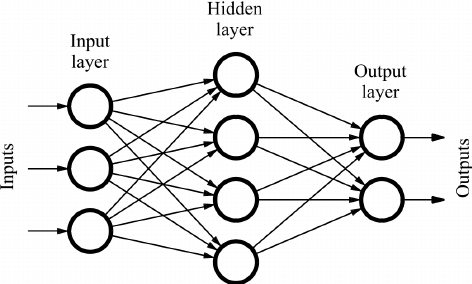
\includegraphics[scale=0.5]{images/DeepNeuralNetwork}
    \caption{A sample of a fully connected deep neural network~\cite{deepNeuralNetworksImage}}
    \label{fig:DeepNeuralNetwork}
\end{figure}

Let us denote $I$ as the input to this model and $O$ as the output.
Let the interacting neuron layers - Input layer,  Hidden layer and the output layers be represented by functions $f_i$, $f_h$, and $f_o$ respectively.
Then the computation of the model can be abstractly represented by

\begin{equation}
O = f_o(f_h(f_i(I)))
\end{equation}

And each function $f$ can be represented by the equation
\begin{equation}
f(I) = \textsc{NonLinearFunction}(\textbf{W} * I + \textbf{b})
\end{equation}

Where the matrix $\textbf{W}$  holds the weights of the connections to the neurons of the current layer and $\textbf{b}$ represents some bias that is added to the outputs of the neurons.
The use of \textsc{NonLinearFunction} makes it possible for the neural network to represent non linear functions.
The overall capacity of the neural network very high and it can be increased by increasing the depth of the network or by increasing the neurons at each layer.

One disadvantages with deep neural network is that they cannot model uncertainty trivially.
One method to do this is to use ensemble of neural networks or the use of specialised loss function with 2 outputs.
Since uncertainty modelling is essential for this thesis,  it is discussed in more detail in the Section~\ref{sec:uncertaintyDeepEnsembles}.

\subsection{Bayesian Neural Networks}
One way to quantify uncertainty is to use stochastic artificial neural networks.
These are also called Bayesian Neural Networks (BNN) because they are trained using Bayesian inference mechanism~\cite{BayesianNeuralNetworks}.
The basic idea is to make sure that the output of any layer in the neural network is stochastic and not a point estimate like in the case of classical artificial neural networks.

In Bayesian neural networks the stochasticity is added by using a stochastic activation function or stochastic weights and biases.
Consider the case where we model a BNN using stochastic weights and biases.
All weights and biases can be represented by a parameter vector $\mathbf{\theta}$.
We then have to define a probability distribution of the parameter vector $p(\theta)$.
This is the prior or Hypothesis in Bayesian jargon.
For example one prior could be a multivariate Gaussian distribution with a mean and a covariance matrix.
Given the training data $D$,  we calculate the new probability distribution to get the posterior distribution $p(\theta | D)$ using Bayes theorem.
Here $D$ is also called evidence.
We do not mention the intricacies of the BNN training procedure as it is out of scope for this thesis.

To understand the estimation of uncertainty,  let the neural network be represented by $f_{\theta}$ for a definite parameter vector $\theta$. 
The uncertainty calculation is done using the following equations
\begin{align*}
\mathbf{\theta}_i \sim p(\mathbf{\theta}| D)  \\
y_i = f_{\mathbf{\theta}_i}(x) \\
\textit{where} \quad i \in \mathbb{I}^+
\end{align*}

First we sample a set of parameters from the posterior probability distribution $p(\theta | D)$.
Using these parameters we calculate multiple values of $y$ for the given input, say $x$.
Using these multiple output values,  one can calculate the mean and the variance of the output of the network.
Note that if the output of the Bayesian Neural Network is a vector we would need to calculate the covariance matrix to get the multivariate variance.

Even though BNNs are theoretically very robust,  practically they are difficult to train.
Firstly,  the exact estimation of the posterior is computationally intractable.
Hence approximate methods like Monte Carlo Markov chains and variational inference methods are used to train the BNNs.
Even these approximations are computationally more expensive than the a classical artificial neural network.
Moreover,  it is not clear from the beginning what prior probability distribution should be used  for the stochastic parameters.
Because of these disadvantages we do not use them for as surrogates in our thesis.

\section{Types of Losses}
\subsection{BO with GP uses negative log likelihood}
It is not clear whether pointwise losses (regression as in GP) are the correct way to model HPO responses, because we only care for the minima regions (best performing configurations), and not for estimating all observations accurately.


\subsection{Ranking Losses}\label{sec:ranklearning}

Consider a set $\mathbb{A} = \{a_1,  a_2,  a_3, ... ,  a_n\}$ where each object $a_i \in \mathbb{D}$ for some domain $\mathbb{D}$.
Let us consider that an object with a lower rank is more preferable than an object with a higher rank.
Then,  the task of ranking the objects of set $\mathbb{A}$ is defined as ordering all objects $a_i \in \mathbb{A}$ such that
$$
\texttt{Rank}(a_i) < \texttt{Rank}(a_j) \iff a_i  \succ a_j
$$

Here \texttt{Rank} of an object $a_i$ is analogous to its position in the ordered list.
This task can be modelled by a machine learning model.
In the most general case the cardinality of $\mathbb{A}$ is not fixed.
Practically building a machine learning model that takes a whole set of an unknown cardinality as input is not trivial.
To keep the model simple,  it is divided into the following components:~\cite{procedureforrankinginintro}
\begin{itemize}
\item Calculation of relevance scores of each $a_i \in \mathbb{A}$.
\item Ordering or sorting of objects based on their relevance scores. 
\end{itemize}

Doing a gradient based optimization for this model is not possible.
This is because sorting is non differentiable and we cannot get a gradient with respect to it.
Hence, to do a gradient based optimization,  we only model the calculation of relevance scores by the machine learning model.
We represent this model by $s$.
We use the letter "s" to signify that we are calculating a "score" for an object. 
$s$ is defined as
$$
s : \mathbb{A} \mapsto \mathbb{R}
$$
One can use $s$ to rank a newly given set of objects.
First the relevant scores of the objects are predicted by $s$.
Thereafter,  using these relevant scores,  the objects are sorted.

Learning a machine learning model requires an optimizing criteria on the output of the model.
This output in our case is the sorted list of objects.
The optimizing criteria in the jargon of machine learning is called a loss function.
Hence,  in our case the loss function can be referred as a \textit{Ranking Loss}.

Ranking losses can be broadly classified into the following types~\cite{RankingLossFirstPaperRead}:
\begin{itemize}
\item  Point-wise ranking losses
\item  Pair-wise ranking losses
\item  List-wise ranking losses
\end{itemize}

In point-wise ranking losses,  the loss function views the ranking problem as a problem of assigning a label to each queried data point.
Hence,  each learning instance is a single object $a_i$ within the set $\mathbb{A}$.
For example,  Li et. al.~\cite{McRank} use point-wise ranking losses for their proposed model called McRank.
Li et.  al.  formulate the ranking problem as a multilevel classification problem.
Each data point is classified independently using soft classification.
The score of an object then is its expected rank.
Similarly,  Cossock et.  al.~\cite{subsetregressionpaper} use point-wise ranking losses for doing subset regression. 
\iffalse
Therefore, the complete scoring function comprises of a multi-level classifier and an external expectation calculation.
\fi

In pair-wise ranking losses,  the loss function's input is a pair of objects.
In this case we learn to model pair-wise preferences.
The loss function tries to separate the input data points as much as possible in the output space by minimising the pair-wise classification error~\cite{pairwisepreferencespaper}.
Examples of models built using pair-wise loss functions are Rankboost~\cite{rankboostpaper} and RankNet~\cite{ranknetpaper}.

In list-wise ranking losses,  a single learning instance is the whole input set i.e all the objects in the input set.
This makes an intuitive sense because we cannot rank the objects independently as an object's rank is relative to the ranks of other objects in a set.
This is the fundamental advantage of list-wise ranking losses when compared to the point-wise and pair-wise losses.
Moreover,  it has been shown by Cao et. al.~\cite{listwisebetter} that training a model with list wise losses gives us a superior model as compared to training with point-wise or pair-wise losses.
The 2 most prominent list-wise loss functions are ListNet~\cite{listwisebetter} and ListMLE~\cite{listmlepaper}.
We discuss and analyse these loss functions in detail in Chapter~\ref{chap:Background}.

\iffalse
We hence use the list wise approach to ranking.
Ranking loss could be the answer in modeling hp optima better.
\fi

\section{Set-modelling with Neural Networks}

In the previous sections we discussed about various types of surrogates that can be used for transferring knowledge in transfer HPO methods.
Training on data from known tasks and then using this trained model for working on unknown tasks, however,  has a major shortcoming conceptually.
Humans do not pre-condition their actions on new tasks only on their previous experiences.
Their pre-conditioning also includes the knowledge of the current task (however little it may be).


To model this concept,  one has to learn to represent and pre-condition knowledge from known tasks in a model.
This makes the model context aware.
If we consider a HP configuration and its evaluation ($\textbf{X}$, $y$) as a single object,  then the group of all the known pairs can be represented as a set.
Here,  $\textbf{X}$ is a feature vector and $y$ is a scalar.
Now our problem is a 2 stage process which includes
\begin{itemize}
\item Representation of a Set
\item Conditioning of our model on the Set Representation.
\end{itemize}


We use Deep Neural networks to represent a set in this thesis because it is a model with  high representational capacity and is easy to train.
Deep Sets by Zaheer et.  al~\cite{deepSets} and Set Transformers by lee et. al~\cite{setTransformer} are two of the interesting researches that we found in the literature.
Since the sophisticated attention mechanisms used in Set transformers were unnecessary for us,  we chose to use the more simple architecture used in Deep Sets.
The next section discusses about these Deep Sets.

% \subsection{Set-transformers}
\subsection{Deep Sets}\label{sec:DeepSets}
Traditionally deep learning or machine learning models learn functions of the following format:
$$
f : \mathbb{R}^d \mapsto \mathbb{R}^k \quad d,k \in \mathbb{I}^+ \quad \textrm{For Regression}
$$
$$
f : \mathbb{R}^d \mapsto \{c_1, c_2, ... c_n\}  \quad \textrm{For Multi-Classification}
$$
which can be thought of transforming objects from the input space to the output space.

For our problem of set latent representation,  the input space changes to a space containing sets (each instance in the space is a set by itself).
The output space however remains similar to either the regression case for regression tasks and classification case for classification tasks.
Consider $\mathbb{X} = \{a,b,  c, ... \}$ be a set containing all possible elements within the sets of the input space.
Then the set representation problem can be defined as:
$$
g : 2^{\mathbb{X}} \mapsto R^k   \quad k \in \mathbb{I}^+ \quad \textrm{For Regression}
$$
$$
g : 2^{\mathbb{X}} \mapsto \{c_1, c_2, ... c_n\}  \quad \textrm{For Multi-Classification}
$$
Where $2^{\mathbb{X}}$ is the power set of $\mathbb{X}$.

2 very important constraints of this problem are
\begin{itemize}
\item Permutation-Invariance constraint: The permutation of the objects within an input set should be irrelevant for the model $g$.
\item Set cardinality invariance constraint: The cardinality of the set can be variable.
Hence our model $g$ should be invariant to the number of elements in the input set.
\end{itemize}

Permutation equivariance is another type of constraint that the deep set paper deals with.
In this constraint the latent space should be equivariant or symmetric to the permutation of the objects in the input set.
This creates issues for our problem because we don't care if our latent space is some symmetric mapping of the input space.
We want the whole set to be mapped definitively to a latent embedding.

\begin{figure}[htb]
\centering
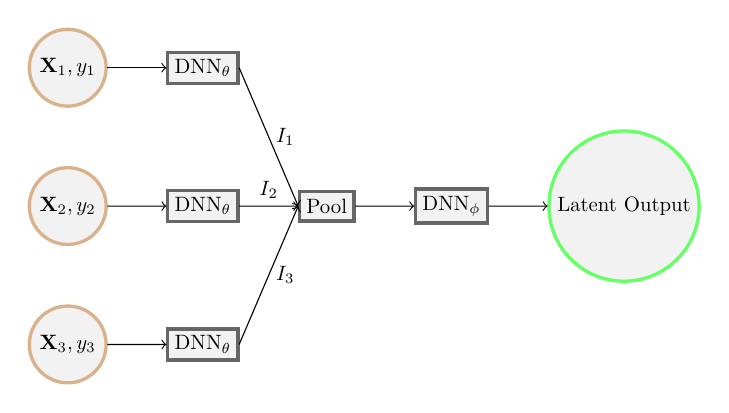
\begin{tikzpicture}[scale=0.75, transform shape,
roundnode/.style={circle, draw=brown!60, fill=black!5, very thick, minimum size=7mm},
roundnodey/.style={circle, draw=green!60, fill=black!5, very thick, minimum size=7mm},
squarednode/.style={rectangle, draw=black!60, fill=black!5, very thick, minimum size=5mm},
]
%Nodes
\node[roundnode]      (X1)                             {$\textbf{X}_1, y_1$};
\node[roundnode]      (X2)                            [below=of X1]     {$\textbf{X}_2, y_2$};
\node[roundnode]      (X3)                            [below=of X2]     {$\textbf{X}_3, y_3$};
\node[squarednode]      (phi1)                      [right=of X1]        {DNN$_{\theta}$};
\node[squarednode]      (phi2)                     [right=of X2]        {DNN$_{\theta}$};
\node[squarednode]      (phi3)                     [right=of X3]        {DNN$_{\theta}$};
\node[squarednode]      (Pool)                     [right=of phi2]     {Pool};
\node[squarednode]      (pho)                      [right=of Pool]     {DNN$_{\phi}$};
\node[roundnodey]      (LatentOutput)         [right=of pho]     {Latent Output};

%Lines
\draw[->] (X1.east) -- (phi1.west);
\draw[->] (X2.east) -- (phi2.west);
\draw[->] (X3.east) -- (phi3.west);
\draw[->] (phi1.east) -- (Pool.west)    node[midway, right] {$I_1$};
\draw[->] (phi2.east) -- (Pool.west)   node[midway, above] {$I_2$};
\draw[->] (phi3.east) -- (Pool.west)   node[midway, right] {$I_3$};
\draw[->] (Pool.east) -- (pho.west);
\draw[->] (pho.east) -- (LatentOutput.west);
\end{tikzpicture}
\caption{Skeletal of the architecture proposed in deep sets}
\label{fig:DeepSetArchitecture}
\end{figure}

Figure~\ref{fig:DeepSetArchitecture} illustrates the architecture proposed by the deep set paper.
We use a set of only 3 objects in the Figure for simplicity.
The architecture passes all the 3 inputs through the a deep neural network independently to get intermediate outputs $I_1$, $I_2$, $I_3$.
To solve the permutation invariance constraint,  any mathematical operation that is commutative and associative is applied on the intermediate outputs.
As long as the pooling operator is permutation invariant, the proposed architecture is also permutation invariant.
Examples of such operators are sum, mean, max etc.

To solve the problem of cardinality constraint we can use the mean operator.
Hence the pooling operation becomes:
$$
\textrm{Pool}(I_1, I_2, I_3) = \frac{ I_1 + I_2 + I_3}{3}
$$

The output of the pool operation is then passed through a different Deep Neural Network to finally get the Latent output.

\iffalse
\section{RGPE}
Read the FSBO paper and write the summary like that or read  the RGPE paper
This section is necessary because our model performs similar to this

\section{TAG}
Read the TAG paper.
Some other model if also necessary and you mention this in your report.
\fi

% \section{Deep Kernel Learning}

\iffalse
Paper: https://arxiv.org/pdf/2101.07667.pdf

Problem Domain: Hyperparameter searching.
Keyword: Use Deep Kernel surrogates

Key points:
    1. Use transfer learning surrogates to get faster convergence
    2. Treat HPO as a few shot learning problem (In the context of transfer learning)
    3. Use kernel k(phi(x), phi(x')) where phi is a neural network that transforms x to a latent vector
    4. Learn parameters of phi(W) and kernel(theta) together based on historical meta data
    5. Fine tune both W and theta based on the given task. If possible use warm start for initialization.
    6. Learn output range variance by creating augumented tasks.

Conceptual points:
    1. The deep kernel learnt does not have any task dependent parameters.
       The task dependent parameters are marginalized out.
       Hence finetuning during test time (after pretraining) should be complete.

Quick note on expected improvement.
    First the mean and variance is calculated for the target Hyperparameter Setting.
    Considering the mean and variance of a particular HP, we calculate the following:
%        Remove y_max from the set of all values of f(x) and lowerbound it by 0.
 %       Multiply the above value with the probability of the gaussian curve N(predicted_mean, predicted_variance)
        For a continous curve we need to integrate.
    Then we get the Expected Improvement for this HP setting.


Gaussian Processes:
    The output is considered to be a random variable.
    When have more than 1 data point, the output becomes a multivariate normal
        The output is a joint gaussian distribution.

Personal points (Probability vs Likelihood)
    Probability and likelihood are reverse in nature.
    Probability starts with a given set of parameters and caculates the probability of a given outcome to occur
    Likelihood starts with a given outcome, and we would like to determine the parameters.

    Marginal likelihood (Likelihood after marginalization of some parameters)
        integrates the effects of parameters that are not of your interest.

Note:
    Warm start is not essential for us. (It is not the main contribution of the paper)

Main motive of deep kernel learning:
    Learn the kernel function in the gaussian process.

How to do implementation with FSBO with HPO-B Metadataset?
There are 16 search spaces (model optmizations here)
    The train test split is already done metatraindata has the training data and metatest data has the test data.
    What about validation?? Really required?
    The search space id can be used for identifying correct search space for test and training data by using:
%        hpobhander.meta_test_data[search_space_id][dataset_id]["X"]
  %      hpobhander.meta_train_data[search_space_id][dataset_id]["X"]

1 ML model optimization
    1 search space (with a unique searchspace id)
        Dataset 1 (with unique dataset id)
        Dataset 2
        Dataset 3

Pretrain the FSBO model with the train split of the dataset. M'
Fine tune it on 1 dataset and evaluate using Expected Improvement
    i.e run loop like the training with the given data.

Did not use strictGP --> Is it a problem?
\fi



\iffalse
This concept is heavily used in domains like document ranking,  web search results  (i.e information retrieval)(and other areas) to rank documents that were retrieved for a given query.
\fi

\iffalse
Main Idea:
    Given a set of objects, we need to rank the objects. (E.g. Ranking documents based on relevance to a query)
    

3 types of ranking functions:


Evalution of learnt RF = Ranking measures.
Relationship of Ranking measures and RLs is unkown.


Main AIM:
    Find relationship between Ranking Measuress and Pointwise/Listwise Ranking Losses.
    Pointsize relationship already clear
    Goal to do the same for pair wize and listwise case.

Proposed IDEA:
    Use an essential loss. (Need more reading)

Loss function understanding:
Pointwise - Try to get the label as per data
Pairwise - Try to separate the labels as much as possible. (Because of -z in all forms of phi).
           It is a classification of 2 objects with a boundary --- Hence the effort to separate things.
Listwise - The anology of this is that of 2 oppposing forces. One the rank of the object. Secondly
           the number of objects below it in the list.
           Loss ===> -rank + number of objects below it.
                If the rank is low and more number of objects are below it ==> Loss > 0 which is not desirable
                On the contrary, if the rank is high it can bear more objects below it as Loss would not be so high.
           Permutation invariance is obtained by using random valid (best case)
%     Doubt. We talk about permutations. It is only possible if #Lables << #DataPoints.
        ==> This is true as we are doing K-Layer classfication.


Ranking Losses:
    Point               Pair            List
    Subset regression   Ranking SVM     ListNET
    McRank              RankBoost       ListMLE
                        RankNet

Brief note on Pairwise approach: from the introduction of https://www.microsoft.com/en-us/research/wp-content/uploads/2016/02/tr-2007-40.pdf
    The data is created by creating (x1, x2) -> label tuples for all possible x1, x2 in the ranked list. The label can be -1, 0, or 1
    ,for instance, if x1 is having lower, equal or higher rank to x2 respectively.

Ranking Measures
    NDCG = K level ratings
    MAP = 2 level ratings

    Read: https://faculty.cc.gatech.edu/~zha/CS8803WST/dcg.pdf
    Read: https://www.microsoft.com/en-us/research/wp-content/uploads/2016/08/letor3.pdf (Page 15 for a clearer picture)
        CG = Cumulated gain (of information)
        DCG = Discounted cumulated gain (of information)
        NDCG = Normalized DCG i.e Divide each position of the DCG by Ideal DCG for the results.
               You get a list of values in [0,1] which lenght of list = number of rankings considered.
        NDCG@k = required real valued function of the ranking measure.

    Question: Only 2 level rankings necessary for our case?

Understanding listwise loss function:
    Queries       Ranking(f(Q, D))      Ground Truth scores
    q1        [d1, d2, d3 ... d10]      [y1, y2, y3 ... y10]
    q2        [d1, d2, d3 ... d15]      [y1, y2, y3 ... y15]
    q3        [d1, d2, d3 ... d7]       [y1, y2, y3 ... y7]

    D = {Set of Documents}
    Q = {Set of Queries}
    f : QxD -> R [Note: Here D is conditioned on Q]. The function is defined for 1 (query, document) pair.

    Point to note - Each feature input = a concatenation of the query vector and the document vector.

    One instance of our training data is (X, Y) where X = {Set of all documents returned by query} Y = {Set of the respective ground
    truth scores}. Basically 1 query is one instance. Hence our loss function has to take in vector of outputs from f.

    Loss = L(Xi , Yi) where Xi and Yi are refer to 1 query qi.
    Full Batch Loss = mean (L(Xi, Yi) for all elements i in the training objects)

    Here f(Q, D) itself is the scoring function that is the main model to be learnt in our framework.

    *** Complete explanation found in Section 3 and Section 4 of paper:
        *** https://www.microsoft.com/en-us/research/wp-content/uploads/2016/02/tr-2007-40.pdf

    * ListNet
    * We need to make sure that f returns scores that are SIMILAR IN RELAVANCE/ORDER to the ground truth scores.
    * This would make the Ranking(f(Q, D)) equal to the ground truth and we would have learnt our ranking function.
    * Note that we do not need to get the exact ground truth scores. Which increases the space of acceptable functions in the
      function space F (Here f belongs to F) we are searching from 1 to INF. i.e It becomes easier to search if we only want a subspace and not the exact function.
    * RANKING is nothing but sorting the results based on their respective scores/relavance (decreasing order)
    * Since the sorting function is non differentiable, the loss function in question should not be composed of the RANKING function.
    * Moreover, leaving the sorting function makes our loss permutation independent by making use of the + permutation invariant operator
      [Check the final step for more clarity on this. Cross entropy uses + operator]
    * This leaves us with 2 lists -
        a. List of scores given by our ranking function f
        b. List of relavance scores given to us by ground truth
    * The loss function finds the distance of these 2 lists.
    * A probabilitic approach is taken so as to take into account for any uncertainities.
%    * The probability of selecting any document can be taken as score_of_document / sum(all document scores) since higher score means
      a more relavant document
    * However the score of the document can negative as well. Hence a strictly positive and increasing funciton phi is taken
%        which makes prob(d) = phi(d) / sum (phi(d_i) for i in Documentsof(QueryGiven))
    * The probability of a permutation is nothing but the probability of selecting one document after another without replacement
      (Reminder: Discrete probability calculation){Which itself becomes a probability distribution i.e sigma = 1}
    * One possible way to find the distance betwen the 2 lists a and b is to find the probabilities of all permutations for a and b
      and compare both the distriputions. 
    * Complexity of this O(n!) ==> Intractible
    * Instead take the probabilities of selecting every document first in any possible permutation. {Which also is a probability 
      distribution i.e sigma = 1}
    * The first selection probability (Top 1 probability in the research paper) for a and b are calculated separately using their
      respective scores.
    * The final Loss for the list = Cross entropy of probability distribution (a) w.r.t that of b.
    * This loss is backpropogated through the network to set the parameters.
%
    ListMLE: http://icml2008.cs.helsinki.fi/papers/167.pdf
    * Main difference is that the loss function used is different.
    * Loss function is intuitive in that they would want to raise the probability of getting the ground truth permutation.
    * They increase the probability of getting the exact (ground truth) permutation using the scores given by f.

    Both the papers use linear network model for some simplicity. But we can use the non-linearity due to available library
        implementations
    Very nice summary of both loss functions section 3.2.1 : https://arxiv.org/pdf/1707.05438.pdf 

Advantages:
    Can be used to select best n configs and then evaluated at random based on the ranks. This is not as trivial to get in other
    places. So there is an amount of parallelism that can be built it.

Best Model for training and ft giving auful resuts - Reason can be that we are selecting a very unfitted model due to too much variation in the validation losses.
Hence we are start only ft best model. Ih the hope that we will get better resutls.
only fine tune best fit is not giving good results. Investigation in progress. 

\fi


\chapter{Background}
\label{chap:Background}

In this chapter, we discuss in detail the fundamental concepts one must grasp to understand the thesis work. We have already talked about the concept of ranking in Section~\ref{sec:ranklearning}.
In this chapter, we take the next step to define the ranking loss functions abstractly.
After that, we discuss the concrete loss functions studied in this thesis.
We also talk about how uncertainty is modeled using Deep Neural Network Ensembles.
Lastly,  we discuss the details of the baseline implementations of Deep Ensembles and FSBO that we did in this thesis.

\section{Ranking Loss functions: Definition}

\iffalse
\begin{table}[ht]
\centering
% spacing in table
% \ra{1.3}  % Commenting this could not get this function right
\begin{tabular}{@{}lr@{}}
  \toprule
  Epochs listsize & Accuracy(within range) Accuracy outside range \\ \midrule
  A    & 82.47 $\pm$ 3.21 \\
  B    & 78.47 $\pm$ 2.43 \\
  C    & 84.30 $\pm$ 2.35 \\
  D    & 86.81 $\pm$ 3.01 \\
  \bottomrule
\end{tabular}

    \caption[Table caption]{\textbf{Sorting accuracy.} Obtained after sorting the numbers based on the scorer's results\\}
    \label{tab:accuracy}
\end{table}
\fi

Consider data in the format shown in table~\ref{tab:dataformat} is given to us.

\begin{table} [ht]
\centering
\begin{tabular}{ | c | c | c | }
  \toprule
  Instance & Object Set & Ground Truth \\ \midrule
% \hline \hline
  1 & $\{a_1, a_2, a_3, ... , a_{10}\}$  & $\{y_1, y_2, y_3, ... , y_{10}\}$  \\
  2 & $\{a'_1, a'_2, a'_3, ... , a'_{15}\}$ & $\{y'_1, y'_2, y'_3, ... , y'_{15}\}$  \\
  3 & $\{a''_1, a''_2, a''_3, ... , a''_{7}\}$ & $\{y''_1, y''_2, y''_3, ... , y''_{7}\}$  \\
  ... & $\{...\}$ & $\{...\}$ \\
  \bottomrule
\end{tabular}
\caption{Data format used to train the scoring function.}
\label {tab:dataformat}
\end{table}
Let each data point $a_i$ be a sample/element from the set $\mathbb{A}$.
Each $y_i$ represents the ground truth preference score of objects belonging to a set $\mathbb{Y}$.
These preference scores of objects are relative to the objects within $\mathbb{A}$.
Let $s$ be the scoring function to be learnt.
Hence, the declaration of $s$ is given by
$$
s : \mathbb{A} \mapsto \mathbb{R}
$$

The signature of the loss function depends on the type of loss we use.
This is because the learning instance is of a different type in point-wise, pair-wise and list-wise losses.
For point-wise loss functions,  each instance learning instance is a single object the loss function and its ground truth.  Its format hence can be defined as:
\begin{equation}
L_{\texttt{point-wise}} : s(\mathbb{A}) \times \mathbb{Y} \mapsto \mathbb{R}
\end{equation}

Similarly,   the pair-wise loss function has each instance as a pair of objects and their corresponding ground truths.  Its format can hence be defined as:

\begin{equation}
L_{\texttt{pair-wise}} : s_1(\mathbb{A}) \times s_2(\mathbb{A}) \times \mathbb{Y}_1 \times \mathbb{Y}_2 \mapsto \mathbb{R}
\end{equation}

For list-wise losses,  one learning instance is a set of objects their corresponding ground truths.
If we take any set $\mathbb{P}$ such that $\mathbb{P} \subseteq \mathbb{A}$,  the declaration of the list wise loss $L$ is hence given by
\begin{equation}
L_{\texttt{list-wise}} : s_1(\mathbb{A}) \times s_2(\mathbb{A}) ...  s_{|\mathbb{A}|}(\mathbb{A}) \times \mathbb{Y}_1 \times \mathbb{Y}_2 \times ...  \mathbb{Y}_{|\mathbb{A}|} \mapsto \mathbb{R}
\end{equation}

We consider the ground truth values to be $\mathbb{R}$ for our analysis of all loss functions.
We have real valued ground truths in our data sets as well.

In the next sections we analyse the loss functions that we we studied in this thesis.
As list-wise loss functions are more advantageous conceptually than others we discuss them in more detail.

\section{Loss function Point Wise: Subset Regression}

For analysing point-wise loss functions,  we take the subset regression loss function proposed by Cossock et. al. ~\cite{subsetregressionpaper} as a reference.
We reused the implementation written by Pobrotyn et. al.~\cite{Pobrotyn2020ContextAwareLT} for our analysis.

This loss function is very similar to the Root Mean Squared Error loss function.
Given a batch containing $a_i$ and their corresponding ground truth values $y_i$ where $0 \leq i \leq N$,  the loss function is of the form
\begin{equation}
L_{\texttt{SubsetRegression}} = \frac{1}{N} \sum\limits_{i=1}^{N} (s(a_i) - \texttt{level}(y_i))^2
\end{equation}

The $\texttt{level}$ is given by the rank of $y_i$ in the current batch.
For example,  consider we have 3 ground truth values $\{y_1 = 0.8, y_2 = 0.9, y_3 = 0.1\}$.
If we consider that a higher $y$ value is better and a lower rank/level is better then 
$\texttt{level}(y_1) = 2,  \texttt{level}(y_2) = 1,  \texttt{level}(y_3) = 3$

To keep the implementation such that the score value is in the same given range as the regression value,  Pobrotyn et. al.~\cite{Pobrotyn2020ContextAwareLT} use a slightly modified version of the loss function which is conceptually the same.
This loss function is given by
\begin{equation}
L_{\texttt{SubsetRegression}} = \frac{1}{N} \sum\limits_{i=1}^{N} (\texttt{distinct\_levels} * s(a_i) - y_i)^2
\end{equation}
Where,  $\texttt{distinct\_levels}$ is the total number of distinct ground truth values in the given batch.

As you can see the loss function does not directly make the scoring
function learn the output regression value.
This property is common across all ranking loss functions.

\section{Loss function pairwise: RankNet}

To analyse how pair-wise loss functions are helpful for the HPO problem,
we study one pairwise loss function namely RankNet~\cite{ranknetpaper}.
We reused the implementation written by Pobrotyn et. al.~\cite{Pobrotyn2020ContextAwareLT} for our analysis.

As we know from table~\ref{tab:dataformat} we are always given a set of values and their corresponding ground truths to train from.
Hence, we have $\{a_1, a_2, a_3..., a_n\}$ inputs and $\{y_1, y_2, y_3..., y_n\}$ ground truths.
As the $L_{\texttt{pair-wise}}$ takes only pairs of values we obtain first the scores of all objects to get $\{s(a_1), s(a_2), s(a_3)..., s(a_n)\}$.
Then,  we form pairs of inputs to the loss function.
After forming the pairs, one instance of the loss function is of the form$\{s(a_1), s(a_2), y_1, y_2\}$.

For the loss function,  the order of the objects in the pair is not relevant.
So,  instead of taking 2 pairs containing the same objects (but in different order) and their ground truth values,  only 1 pair is taken such that $s(a_1) - s(a_2) > 0$.
This makes the implementation easier.
Let the actual probability of $a_1 \succ a_2$ is given by $P^*$,  and the predicted value of the same is given by $P$.
Then the pairwise loss is nothing but the cross entropy loss given by
\begin{equation}
L_{\texttt{RankNet}} = \texttt{C.E.Loss} = -P^*\log P - (1 - P^*)\log(1-P)
\end{equation}

To calculate the predicted probability the following function was used
\begin{equation}
\label{eq:pairwiseprobability}
P(a_1 \succ a_2) = \frac{e^{s(a_1) - s(a_2)}}{1 + e^{s(a_1) - s(a_2)} }
\end{equation}

We have also seen that the pair-wise loss function only tries to classify the input objects.
This means we only need to know if one object is better than the other from the ground truth values.
Hence a binary cross entry loss function is used instead of a general one in the implementation.
So $P^* \in \{0, 1\}$ in our case.

\section{Loss function list-wise: ListNet}

In this section we try to intuitively explain the ListNet idea proposed in~\cite{listwisebetter}.
Our objective is to learn the scoring function $s$ such that it returns scores that are similar in relevance/order when compared to the ground truth scores.
That is to say
$$
y_3 < y_{12} < y_1 \implies s(a_3) < s(a_{12}) < s(a_1)
$$
This would make the ranking of the objects equal to the ranking obtained by using the ground truth values.
Note that we do not need to get the exact ground truth scores.
This increases the number of acceptable functions that can be learnt by increasing the target function space.
This makes it easier to learn the scoring function.

Ranking is obtained by sorting the objects based on their respective scores.
Note that the sort functionality is non differentiable hence it is not a 
part of the ranking loss function.
Our loss function needs to be constructed using the following 2 lists:
\begin{itemize}
\item List of scores given by scoring function $s$.
\item List of scores given to us by ground truth.
\end{itemize}

The loss function must find some sort of a distance between the 2 given lists.
It then can reduce the distance by changing the parameters of the scoring function.

In ListNet,  a probabilistic approach is taken so as to account for any uncertainties in the ground truth values.
Consider selecting an object from the input set with a probability
\begin{equation}
P = \frac{s(a)}{\Sigma_i s(a_i)} \;\;\; \forall i \in \{1, 2, 3, ...,  |\mathbb{P}|\}
\end{equation}

This make intuitive sense because the probability of selecting an object should be higher if it more relenvant and vise-versa.
Note that the score of any object by the scoring function can negative as well.
Therefore the score is passed through a strictly positive and increasing function $\phi$.
This changes the probability to
\begin{equation}\label{eq:objselection}
P = \frac{\phi(s(a))}{\Sigma_i \phi(s(a_i))} \;\;\; \forall i \in \{1, 2, 3, ...,  |\mathbb{P}|\}
\end{equation}

Equation~\ref{eq:objselection} is also referred to as top 1 probability of an object in~\cite{listwisebetter}.
This is because this gives the probability of ranking the object first when we are calculating the permutation probability of given list.

The proposed way to find the distance between 2 lists in ListNet is
\begin{itemize}
\item Find the top 1 probabilities of each object using the scores given by the scoring function.
\item Using the ground truth values,  find similar top 1 probabilities.
\item The cross entropy between the 2 entities gives us the "distance" between the 2 lists.
\end{itemize}

Let $P_{s(a)}$ represent the top 1 probability of an object using the scores given by the scoring function.
Similarly,   let $P_y$ represent the top 1 probability using its ground truth value.
The cross entropy used as a loss in ListNet is given by
\begin{equation}
L(\textbf{y},  {s(\textbf{a})}) = - \Sigma_i P_{s(a_i)} \log P_{y_i}
\end{equation}
Where $\textbf{y}$ and $s(\textbf{a})$ represent the ground truth values and the scores given by the scoring function.

\iffalse

\fi

\section{Loss function: ListMLE}\label{sec:listMLE}

ListMLE loss stands for, "List Maximum Likelihood Estimation" loss.
It is another type of list loss function that is similar to listNet.
As in ListNet,  the probability of selecting an object from the list is taken the same as given in equation~\ref{eq:objselection}.
However,  the final loss used in MLE is not cross entropy.
Rather it maximizes a likelihood estimation as the name suggests.

Let $\pi$ define any permutation of a list.
The probability of a permutation is nothing but the probability of selecting one document after another without replacement.
In our case the permutation probability of selecting 1 permutation using the selection probabilities given by equation~\ref{eq:objselection}  is~\cite{listwisebetter}
\begin{equation}\label{eq:firstMLEequation}
P_{\pi} = \prod\limits_{j=1}^{k} \frac{\phi(s(\pi_j))}{ \sum\limits_{t=j}^k \phi(s(\pi_k))}
\end{equation}
where $\pi_i$ is the object at position $i$ in the permutation $\pi$.

Applying log to the above equation gives us
\begin{equation}
\log P_{\pi} = \sum\limits_{j=1}^{k} \log \frac{\phi(s(\pi_j))}{ \sum\limits_{t=j}^k \phi(s(\pi_k))}
\end{equation}

However,  the question remains which permutation to use?
The best permutation for the given set of objects would be according to the true scores of the objects.
More precisely,  it would be the objects ordered in the descending order of their relevance scores.
Let this permutation be represented by $\pi^*$.
Hence our probability equation becomes
\begin{equation}
\log P_{\pi^*} = \sum\limits_{j=1}^{k} \log \frac{\phi(s(\pi^*_j))}{ \sum\limits_{t=j}^k \phi(s(\pi^*_k))}
\end{equation}

ListMLE maximizes this probability.
Since most we generally minimize the objective function,  the loss function of ListMLE is given by
\begin{equation}
L_{mle} = - \log P_{\pi^*}
\end{equation}
Expanding the right hand side of the equation gives us the final loss function that has to be minimised by any algorithm that uses ListMLE

\begin{equation}
L_{mle} = -  \sum\limits_{j=1}^{k} \log \frac{\phi(s(\pi^*_j))}{ \sum\limits_{t=j}^k \phi(s(\pi^*_k))}
\end{equation}


Notice that in the calculation of the loss, the true score values of the objects are unused.
Which means that the actual scores of the objects do not matter.
The only constraint is that the scores must have the values that give the same permutation.
Even uneven scaling of the actual scores does not affect the output as long as the constraint is maintained.

In the case of ListNet,  however,  the true scores do matter.
The probability of selecting objects according to their true scores is used.
Hence the result is invariant only to linear scaling.

This advantage makes listMLE loss function superior to the ListNet as it makes the target space of functions bigger and hence the convergence can be quicker.
Because of this advantage we use ListMLE as a list loss function in our thesis.

\section{Position Enhanced Ranking}\label{sec:positionEnhancedRanking}

In many problem domains that use the ranking concept,  it may not be important that each object be placed at exact location as induced by its relevance.
For example,  when a search engine ranks its search results, it is more important to find the most important results and rank them correctly than to order the least important results correctly.

This is also the case in the problem of ranking HP configurations when the ranking model is used as a surrogate in an SMBO process.
In this process,  the ranking surrogate is only needed to obtain the most important HP configuration at each step in the optimization cycle.

Lan et al.  discuss this problem in detail in their paper,  "Position-Aware ListMLE: A Sequential Learning Process for Ranking"~\cite{positionawarerankinglistmle}.
However,  they reformulate the problem as a sequential learning process.
A more accessible approach is to weight each object component in our ListMLE by any decrease function $c$~\cite{TRLWO}.
This is possible because the listMLE loss function is in the form of a summation.
Hence the weighted ListMLE function is given by:

\begin{equation}
L_{mle} = -  \sum\limits_{j=1}^{k} c(j) \log \frac{\phi(s(\pi^*_j))}{ \sum\limits_{t=j}^k \phi(s(\pi^*_k))}
\end{equation}
Where $c(j)$ gives the weight of the rank j in the ordered list.
This is approach used in our model to improve our ranking loss function.
The type of decreasing function to use is discussed in more detail in chapter 4.
Note that it is also possible for using the weighting in the ListNet case as ListNET and ListMLE have similar forms.

\section{Uncertainty modelling using Deep Ensembles}\label{sec:uncertaintyDeepEnsembles}

Deep Neural Networks (DNNs) are machine learning models with very high representational capacity~\cite{Goodfellow-et-al-2016}.
Due to this property,  one can use them as surrogates for HPO objective functions.
But the issue is that DNNs do not quantify uncertainty trivially.
In fact the results can be seen as overconfident.
If used in any HPO optimization algorithm as surrogate,  such overconfident wrong predictions cause a lot of computational overhead by predicting inefficient HP configurations.

We are discussing in detail this concept because we use deep neural networks as a scoring function in our proposed ranking loss surrogate model.
Uncertainty estimation qualities of a surrogate have high importances especially if they are used in techniques like SBMO.
As the proposed model is studied as a surrogate in the SMBO technique,  we need to study how to model uncertainty efficiently using the underlying DNN architecture.

In the current literature,  uncertainty quantification methods using deep neural networks can be broadly classified into the following methods:
\begin{itemize}
\item Bayesian Neural networks~\cite{Goan-2020}.
\item Ensemble Approach using monte carlo drop out~\cite{JMLR:v15:srivastava14a}.
\item Ensemble approach using multiple neural networks.
\end{itemize}

In Bayesian neural network(BNN),  a prior over weights and biases is specified during the initialization of the BNN.
Given the data,  a posterior predictive distribution is calculated for all the parameters of the network (Weights and Biases).
One issue with this approach is that BNNs are very complex and difficult to train. 

Monte Carlo drop out is a regularization technique used during the training of neural networks.
With a certain probability,  connections between neurons are dropped.
Using this technique one obtains possibly $2^N$ neural networks where $N$ is the number of connections
in the artificial neural network.
We can get an ensemble of high capacity models for free.
It is normally only used during training to obtain regularization.

However,  if one uses Monte Carlo dropout during the evaluation,  we can get multiple results from the same input using this approach.
Given input $x$ and output $y = \textrm{NN}(x)$.  If we have $m$ neural networks obtained using Monte Carlo dropout,  we get $\{y_1, y_2... y_m\}$ outputs,  we can obtain the mean and variance of 
\begin{equation}\label{eq:simpleDNNensemble}
y_\textrm{mean} = \frac{\Sigma y}{m}  \;\;\;\;\;  y_\textrm{variance} =\frac{\Sigma(y - y_{mean})^2}{m-1}
\end{equation}
Please note that the $m-1$ in the denominator is due to Bessel’s Correction~\cite{besselcorrection} to reduce the bias in estimation.


Lakshminarayana et al.~\cite{DeepEnsemblePaper} propose another method to predict uncertainty using deep neural networks.
They propose that the uncertainty prediction can be done directly using a single neural network.
This is possible if we assume that the underlying uncertainty is a Gaussian distribution.
With this assumption, the neural network would have 2 outputs instead of one.
One for the mean of the prediction, say $\mu$, and the other for the variance,  say $\sigma^2$
 of the prediction.
One important point to note is that the variance cannot really be negative.
This is made sure by the authors to pass the output of the neural network through a strictly positive "softplus" function.
 
The authors propose to optimize the following loss function
$$
L_{de} = \frac{\log \sigma^2 }{2} + \frac{(y - \mu)^2}{2\sigma^2} + k
$$
Where both the outputs are some functions of the DNN parameters ($\theta$) and the input ($\textbf{x}$) i.e $\sigma^2 = f(\theta,  \textbf{x})$ and $\mu = g(\theta, \textbf{x})$.
Here, the back propagation finds and updates the parameters $\theta$ using the partial derivative:
$$
\frac{\partial L}{\partial \theta}
$$


We use this loss function to build deep ensemble surrogates for the HPO.
The prediction of uncertainty using ranking losses is however done using the simple ensemble approach given in equation~\ref{eq:simpleDNNensemble}.
This is because the integration of the loss function which learns both the mean and variance with the ranking loss functions is non trivial.

One simple approach is to simply use a combination of losses like
$$
L_{\textrm{total}} = L_{mse} + L_{de}
$$
However such loss functions would need a thorough theoretical analysis which is out of the scope of this thesis.
Hence we do not use this approach on our proposed model.

As there are are multiple neural networks, each predicting its own Gaussian distribution,
there needs to be a mechanism to integrate the results.
This is done using a mixture of Gaussian Distributions.
If there are $m$ neural networks in the ensemble,  the mean and variance are given by
$$
\mu_{final} =  \frac{\sum\limits_{i=1}^{m} \mu_i}{m} \quad \textrm{and} \quad \sigma_{final}^2 = \frac{\sum\limits_{i=1}^{m} (\sigma_i^2 + \mu_i^2) - \mu_{final}^2}{m}
$$

\section{Baselines}

In this thesis,  2 HPO techniques were implemented before studying the proposed model - Deep Ensembles and Few Shot Bayesian Optimization (FSBO).
Deep Ensembles were used as surrogates in the SMBO optimization.
They were studied with with 2 main objectives in mind.
First to study how uncertainty is estimated using Deep Neural Networks using the approach proposed by~\cite{DeepEnsemblePaper}.
This was a pre-requisite to implement the uncertainty in our proposed model as we use deep neural networks as a scorer in our model. 
Second to understand how a non transfer technique like GP would work for our given problem.
Note,  it is also possible to make the Deep Ensemble surrogate a transfer technique by meta training it before using it in the optimization cycle.

The second technique implemented was FSBO.
We choose this because as this gave the state of the art results on the HPO-B benchmark that we use.
(The benchmark is discussed in the later chapters).
Studying FSBO also gave us an idea on how to implement the transfer mechanism in our proposed model.
In addition to this we used Random search and GP as standard baselines for result comparison.

Both these FSBO and DE have built in capability for uncertainty estimation.
Hence we have to use an acquisition function during the optimization cycle of SMBO.
Expected improvement was used in all models that deal with uncertainty.
This is to maintain consistency in results across all the models.
Further more it also has advantages on other acquisition function~\cite{Jones1998}.


The following 2 sections discuss the implementation details of the baselines methods used in our thesis.

\subsection{Deep Ensemble}

As previously mentioned Deep Ensembles were implemented according~\cite{DeepEnsemblePaper} as a non transfer surrogate.
Hence,  there was no meta-training done for the Deep Ensembles.
Consequently the usage of DE as a surrogate was quite similar to that of Gaussian processes.
SMBO with deep ensemble was implemented as shown in algorithm~\ref{alg:deepEnsembleFinetuning}~\cite{pineda2021hpob}.

\begin{algorithm}[H]
\caption{SMBO with Deep Ensemble surrogate}
\label{alg:deepEnsembleFinetuning}
\begin{algorithmic}
    \State $X_{known},  Y_{known} \gets$ Initial HP configurations.
    \State $X_{pending} \gets$ HP configurations to evaluate.
    \State $k \gets$ Number of evaluation cycles
    \For{$i < k$}
        \State DE $\gets$ Randomly initialize Neural Networks. 
        \For {$nn \in$ DE}  \Comment{Can be trained in parallel}
            \State train($nn$) with $X_{known},  Y_{known}$
        \EndFor
        \State $EI_{scores} \gets$ EI( $X_{pending}$ ) \Comment{Expected Improvement scores}
        \State $x^* \gets $ best $(EI_{scores})$
        \State $y^* \gets f(x^*)$ \Comment{HP objective function evaluation}
        \State $X_{known} \gets X_{known} \cup x^*$
        \State $Y_{known} \gets Y_{known} \cup y^*$
        \State $X_{pending} \gets X_{pending} \setminus x^*$ 
        \State $i \gets i + 1$
    \EndFor
    
\end{algorithmic}
\end{algorithm}

We use similar procedures like Algorithm~\ref{alg:deepEnsembleFinetuning} for other models i.e FSOB implementation and the proposed Ranking Loss surrogate model.
The only difference is that the surrogate and its training step differ with different methods.

A few points are worth noting here.
First,  we see that the algorithm evaluates a set of discrete HP configurations in the HP search space.
This is the same approach we take when we apply our model because the ranking concept we use requires a set of defined objects.
The advantage of using this approach is that there is no restriction on the type of search space we optimize.
It may be discrete or continuous.
If it is continuous,  we only have to discretize it upto a required granularity based on our computational resources.

Secondly,  we see that at each evaluation cycle,  a new set of neural networks are trained.
Old trained neural networks are discarded.
This rationale behind this is discussed in chapter 4.
We also use this sort of initialization in other models.
Finally,  as the neural networks are independent of each other,  they can be trained in parallel.
This makes the usage of this model scalable.

One question that remains to be answered is what sort of architecture is used by our neural networks.
For this 2 architectures were analysed - undivided neural network as shown in Figure~\ref{fig:undividedarchitecture} and a neural network divided at its tail as shown in Figure~\ref{fig:dividedarchitecture}
\begin{figure}[htb]
\centering
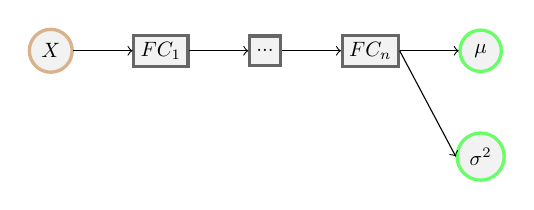
\begin{tikzpicture}[scale=0.75, transform shape,
roundnode/.style={circle, draw=brown!60, fill=black!5, very thick, minimum size=7mm},
roundnodey/.style={circle, draw=green!60, fill=black!5, very thick, minimum size=7mm},
squarednode/.style={rectangle, draw=black!60, fill=black!5, very thick, minimum size=5mm},
]
%Nodes
\node[roundnode]      (X)                             {$X$};
\node[squarednode]      (FC1)                      [right=of X]        {$FC_1$};
\node[squarednode]      (FCmiddle)             [right=of FC1]        {...};
\node[squarednode]      (FCn)                      [right=of FCmiddle]        {$FC_n$};
\node[roundnodey]      (mean)                             [right=of FCn] {$\mu$};
\node[roundnodey]      (variance)                             [below=of mean] {$\sigma^2$};

%Lines
\draw[->] (X.east) -- (FC1.west);
\draw[->] (FC1.east) -- (FCmiddle.west);
\draw[->] (FCmiddle.east) -- (FCn.west);
\draw[->] (FCn.east) -- (mean.west);
\draw[->] (FCn.east) -- (variance.west);
\end{tikzpicture}
\caption{Example of an undivided Neural Network architecture}
\label{fig:undividedarchitecture}
\end{figure}

\begin{figure}[htb]
\centering
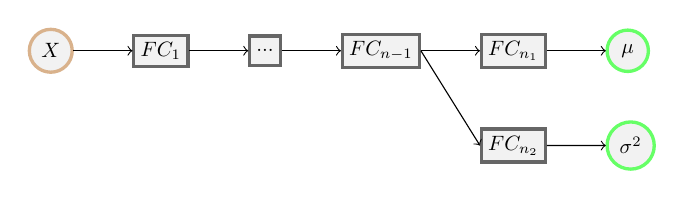
\begin{tikzpicture}[scale=0.75, transform shape,
roundnode/.style={circle, draw=brown!60, fill=black!5, very thick, minimum size=7mm},
roundnodey/.style={circle, draw=green!60, fill=black!5, very thick, minimum size=7mm},
squarednode/.style={rectangle, draw=black!60, fill=black!5, very thick, minimum size=5mm},
]
%Nodes
\node[roundnode]      (X)                             {$X$};
\node[squarednode]      (FC1)                      [right=of X]        {$FC_1$};
\node[squarednode]      (FCmiddle)             [right=of FC1]        {...};
\node[squarednode]      (FCpenaltimate)             [right=of FCmiddle]        {$FC_{n-1}$};
\node[squarednode]      (FCn1)                      [right=of FCpenaltimate]        {$FC_{n_1}$};
\node[squarednode]      (FCn2)                      [below=of FCn1]        {$FC_{n_2}$};
\node[roundnodey]      (mean)                             [right=of FCn1] {$\mu$};
\node[roundnodey]      (variance)                             [right=of FCn2] {$\sigma^2$};

%Lines
\draw[->] (X.east) -- (FC1.west);
\draw[->] (FC1.east) -- (FCmiddle.west);
\draw[->] (FCmiddle.east) -- (FCpenaltimate.west);
\draw[->] (FCpenaltimate.east) -- (FCn1.west);
\draw[->] (FCpenaltimate.east) -- (FCn2.west);
\draw[->] (FCn1.east) -- (mean.west);
\draw[->] (FCn2.east) -- (variance.west);
\end{tikzpicture}
\caption{Example of a divided Neural Network architecture}
\label{fig:dividedarchitecture}
\end{figure}

In both these figures,  FC stands for fully connected layers.
As the undivided architecture is closer to the neural network used in the proposed ranking loss surrogate model,  we used it for the sake of consistent comparison.
3 Fully connected layers of 32 neurons each were used for each neural network.
All neural networks used the same architecture. 
The training was done using the the Adam optimizer with full batch gradients.
This is because the number of data points in the evaluation cycle are very few.
Each neural network was trained for a 1000 epochs with a learning rate of 0.02.
We do not use adversarial examples as proposed in the deep ensemble paper because it was giving bad results.

\subsection{FSBO}
\label{sec:FSBOBackground}
Few Shot Bayesian Optimization (FSBO) is a transfer learning HPO method that utilizes a meta learnt surrogate for knowledge transfer mechanism.
It reformulates the problem into few shot learning task.
In the context of our problem,  this means meta learning thoroughly from the existing meta data and then adapting to the new task at evaluation cycle by fine tuning a few training epochs.
Therefore the following 2 steps are required to be done in a chronological order
\begin{itemize}
\item Meta training - For knowledge transfer.
\item Fine tuning - For few shot learning.
\end{itemize}

For the purpose of knowledge transfer, the authors make use of a deep kernel surrogate proposed in by wilson et al~\cite{pmlr-v51-wilson16}.
Here,  a neural network is used to transform points in the HP search space to a latent space.
Kernels are then applied to this latent space in a Guassinan process to obtain a probabilistic evaluation.
The deep kernel kernel can be represented as~\cite{fsbopaper}
$$
k(\phi(\textbf{x}, \textbf{w})  ,   \phi(\textbf{x'}, \textbf{w}) |  \mathbf{\theta})
$$
Where $\textbf{x}$ and $\textbf{x'}$ are HP inputs in the original search space,
$\mathbf{\theta}$ and $\textbf{w}$ are parameters of kernel $k$ and the neural network $\phi$.
We used the implementation of deep kernels provided by Patacchiola et al.~\cite{patacchiola2020bayesian} in this thesis.

During the meta training step, we train our surrogate by learning the parameters $\mathbf{\theta}$ and $\textbf{w}$.
A New FSBO model and consequently new surrogate parameters have to be learnt for every new search space.
This is the case even if the input dimensions are of the search space domain are the same.
This is because every HP search space represents different machine learning model and hence has a different HP response surface.
During training we first used an RBF kernel and then used a matern $\frac{5}{2}$ kernel.
A fully connected neural network was used to obtain the latent space representation.

If an assumption is made that the knowledge from the meta data is enough to predict the best HP configuration across all future dataset,  the fine tuning step may be skipped.
However,  this is rarely the case as there are always variations in new dataset (Even though the model being optimised is the same).
Therefore,  the hyper parameter response surface would also be different.

The optimization algorithm in the case of FSBO is similar to Algorithm~\ref{alg:deepEnsembleFinetuning} with a minor change.
The acquisition function used in this model is also expected improvement.
The concept of restarting the fine tuning each time is also proposed in the FSBO paper~\cite{fsbopaper}.
The difference here is that at each evaluation step,  the stored model is loaded anew and fine tuned before using it for predicting the best model.
The restart happens from the meta trained FSBO model and not from a randomly initialized model as in the case of Deep Ensembles.

In our implementation,  Adam optimizer was used in both the training and fine tuning steps.
Note,  however,  that the learning rate of the kernel parameters and the neural network parameters were identical.
The learning rate used for meta-training was 0.0001 and that used for fine tuning was 0.03 different.
We utilized cosine annealing during the fine tuning cycle.
The rationale for using this is discussed in detailed in chapter 4.

We used early stopping mechanism for meta training because we wanted to avoid huge computation costs and over fitting of the model during training.
We took advantage of the split of meta-validation data to do the early stopping.
We saved the best model in our implementation and if the validation loss went greater than lowest validation loss.
The training was stopped if the training error was consistently higher than the validation error for a set number of epochs.
In our case it was 10 epochs but this is easily configurable.

\iffalse
\subsubsection{Implementation issues}
After completing the own implementation,  we found that the results obtained were not in par with the paper.
For this reason, the results are used only for the first stage.
The results already present in the benchmarking data of~\cite{pineda2021hpob} were used for comparing this result with our implementation.
\fi

% \section{Evaluation Strategy}



\chapter{Method}\label{chap:ProposedIdea}

% \section{Proposed Idea: : Ranking Loss Surrogates}

The choice of the surrogate used in a model-based optimization algorithm is crucial. This is because the selected surrogate directly impacts the optimization performance.
Moreover, we also have to answer critical questions prior to its selection. Some of them are - Does the surrogate have enough representative capacity?
Does it have the capability of representing uncertainty?
How is the surrogate learned?

In the quest to improve HPO surrogates,  we propose and analyze a new type of surrogate model based on the concept of ranking:
There are two primary components of our proposed idea

\begin{itemize}
\item The learning mechanism of the surrogate model.
\item The surrogate model itself.
\end{itemize}

This chapter discusses in detail both these components.
We initially use a model with sufficient representational capacity and a capability to represent uncertainty.
An excellent model with these properties is a Deep ensemble; hence, we use it as a model.
We then analyze and implement the proposed learning algorithm that uses the concept of ranking.
Finally, we make the proposed ranking loss surrogate context-aware by integrating deep sets into the Deep ensemble architecture.
We use SMBO as a reference HPO algorithm for our study.



\section{Deep Ranker}
\label{sec:BasicScoringModelDNN}

In order to discuss the implementation details of ranking loss functions,  we need to understand how a basic ranker works.
A basic ranker consists of a Deep Neural Network that outputs real-valued scores $\textbf{s}$ for a batch of inputs, say $\textbf{X}$.
These scores are used to rank the batch of inputs, with the highest score getting the lowest rank.
Our thesis assumes that a lower rank is better than a higher one.
Figure~\ref{fig:basicScoringModel} depicts the architecture of a basic ranker.

\begin{figure}[htb]
\centering
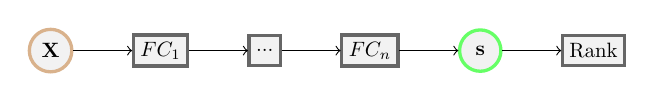
\begin{tikzpicture}[scale=0.75, transform shape,
roundnode/.style={circle, draw=brown!60, fill=black!5, very thick, minimum size=7mm},
roundnodey/.style={circle, draw=green!60, fill=black!5, very thick, minimum size=7mm},
squarednode/.style={rectangle, draw=black!60, fill=black!5, very thick, minimum size=5mm},
]
%Nodes
\node[roundnode]      (X)                             {$\textbf{X}$};
\node[squarednode]      (FC1)                      [right=of X]        {$FC_1$};
\node[squarednode]      (FCmiddle)             [right=of FC1]        {...};
\node[squarednode]      (FCn)                      [right=of FCmiddle]        {$FC_n$};
\node[roundnodey]      (y)                             [right=of FCn] {$\textbf{s}$};
\node[squarednode]      (Rank)                      [right=of y]        {Rank};

%Lines
\draw[->] (X.east) -- (FC1.west);
\draw[->] (FC1.east) -- (FCmiddle.west);
\draw[->] (FCmiddle.east) -- (FCn.west);
\draw[->] (FCn.east) -- (y.west);
\draw[->] (y.east) -- (Rank.west);
\end{tikzpicture}
\caption{Basic ranker.}
\label{fig:basicScoringModel}
\end{figure}

This DNN architecture is very similar to the DNNs used in the Deep Ensemble baseline implementation (Figure~\ref{fig:undividedarchitecture}).
The difference between the 2 is that Figure~\ref{fig:undividedarchitecture} had 2 outputs whereas Figure~\ref{fig:basicScoringModel} has one output.
In addition, there is one extra but crucial step of ranking in the basic ranker.
Since we use a Deep Neural Network to get the scores before ranking the inputs,  we may also refer to this architecture as a Deep Ranker.

Let  \{\textbf{X}, \textbf{y}\} be the training data used for training a generic machine learning model.
Most loss functions utilize the values present in \textbf{y} as a reference for training the ML model.
After the training completes, the range of the outputs of the learned ML model is not vastly different from the range of the actual output values.
However, when we use a ranking loss function to train the ML model, we cannot guarantee this. This is because the ranking loss calculates the loss in the ranking space instead of the output space.
The only thing that matters for ranking loss functions is that the objects should be ranked in the correct order.
Hence the score range of the basic ranker can be arbitrary.
The only exception is a point-loss function called Subset Regression.
This is because subset regression directly learns the rank instead of using the output score $s$ to rank the batch of inputs.

There may be occasions where the score range of the basic ranker needs to be controlled.
For further discussion on this please refer Appendix~\ref{chap:OutputRangeControl}.


\subsection{Uncertainty implementation using Deep Ensembles}\label{sec:UncertaintyImplementation}

We know from Section~\ref{sec:hpoConstraints} that the evaluation of the target objective function in HPO is noisy.
Hence it is essential for any surrogate that models this objective function to have the capability of estimating uncertainty.
The uncertainty estimation becomes more critical in a sequential HPO algorithm like SMBO.
In the first steps of SMBO, we do not have enough data to build or finetune the surrogate.
Using a surrogate without uncertainty in the initial steps may give wrong results with high confidence.
This is not good in a sequential process because selecting subsequent HP configurations depends on the previously selected HP configurations.
For this reason, a model with uncertainty (if estimated correctly) is superior to other models.


We now integrate multiple basic rankers (or Deep Rankers) to build an ensemble of rankers.
Using this ensemble, we can estimate uncertainty in the rank prediction.
Figure~\ref{fig:proposeModelUncertainty} shows the architecture of the ensemble of basic rankers.

\begin{figure}[htb]
\centering
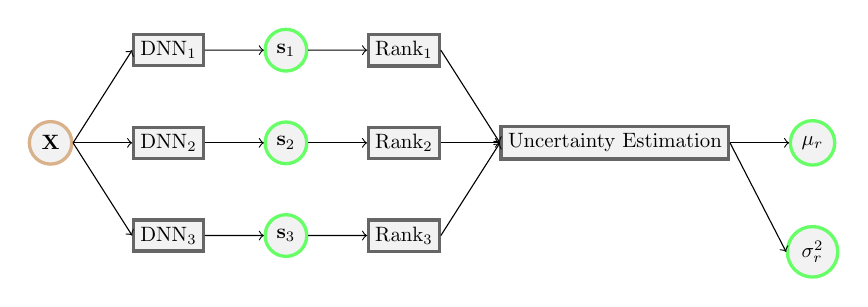
\begin{tikzpicture}[scale=0.75, transform shape,
roundnode/.style={circle, draw=brown!60, fill=black!5, very thick, minimum size=7mm},
roundnodey/.style={circle, draw=green!60, fill=black!5, very thick, minimum size=7mm},
squarednode/.style={rectangle, draw=black!60, fill=black!5, very thick, minimum size=5mm},
]
%Nodes
\node[roundnode]          (X)                                           {$\textbf{X}$};
\node[squarednode]      (DNN2)                      [right=of X]        {DNN$_2$};
\node[squarednode]      (DNN1)                      [above=of DNN2]                    {DNN$_1$};
\node[squarednode]      (DNN3)                      [below=of DNN2]                    {DNN$_3$};
\node[roundnodey]        (y1)                             [right=of DNN1] {$\textbf{s}_1$};
\node[roundnodey]        (y2)                             [right=of DNN2] {$\textbf{s}_2$};
\node[roundnodey]        (y3)                             [right=of DNN3] {$\textbf{s}_3$};
\node[squarednode]      (Rank1)                             [right=of y1] {Rank$_1$};
\node[squarednode]      (Rank2)                             [right=of y2] {Rank$_2$};
\node[squarednode]      (Rank3)                             [right=of y3] {Rank$_3$};
\node[squarednode]      (UncertaintyEstimation)                             [right=of Rank2] {Uncertainty Estimation};
\node[roundnodey]        (mus)                             [right=of UncertaintyEstimation] {$\mu_r$};
\node[roundnodey]        (sigmas)                             [below=of mus] {$\sigma^2_r$};

%Lines
\draw[->] (X.east) -- (DNN1.west);
\draw[->] (X.east) -- (DNN2.west);
\draw[->] (X.east) -- (DNN3.west);
\draw[->] (DNN1.east) -- (y1.west);
\draw[->] (DNN2.east) -- (y2.west);
\draw[->] (DNN3.east) -- (y3.west);
\draw[->] (y1.east) -- (Rank1.west);
\draw[->] (y2.east) -- (Rank2.west);
\draw[->] (y3.east) -- (Rank3.west);
\draw[->] (Rank1.east) -- (UncertaintyEstimation.west);
\draw[->] (Rank2.east) -- (UncertaintyEstimation.west);
\draw[->] (Rank3.east) -- (UncertaintyEstimation.west);
\draw[->] (UncertaintyEstimation.east) -- (mus.west);
\draw[->] (UncertaintyEstimation.east) -- (sigmas.west);

\end{tikzpicture}
\caption{Ensemble of Basic Rankers.}
\label{fig:proposeModelUncertainty}
\end{figure}


In Section~\ref{sec:uncertaintyDeepEnsembles}, uncertainty is estimated by calculating the mean and the variance of the DDN's output scores. This calculation of uncertainty is in the output space of the ensemble.
In the case of ranking loss surrogates, uncertainty estimation is a  little different.
As we are primarily interested in ranking the HP configurations, individual scores and their distributions have less meaning for us.
Instead, we are concerned about the uncertainty in the predicted rank.
In other words, we want to calculate the uncertainty in the rank space.

We first calculate the rank of each HP configuration in the batch as per the rankers' output scores.
Using these ranks, we calculate the mean rank $\mu_r$ and variance in the rank $\sigma^2_r$.
Any acquisition function that uses a ranking model needs to use this "ranking distribution" instead of the output score distribution.

\iffalse
After adding Deep Sets, we train all of them together due to the architectural requirement.
\fi

\iffalse
Hence for example if we are using ListMLE,  our loss function would be given by
\begin{equation}\label{eq:overflowissue}
L_{mle} = -  \sum\limits_{j=1}^{k} \log \frac{\exp(\mu(\pi^*_j))}{ \sum\limits_{t=j}^k \exp(\mu(\pi^*_k))}
\end{equation}
\fi

\subsection{Acquisition function in the Ranking space}
When doing HP optimization using ranking loss surrogates, it is essential to note that the ranking of an HP configuration is relative.
A configuration can have different ranks based on the batch in which it is located.
The expected rank of a configuration is not defined in absolute terms. It is always conditioned on other configurations in the ranking batch.
Due to this property, using the predicted uncertainty in the ranking space is tricky.

Moreover, using well-defined acquisition functions like Expected Improvement (EI) is not trivial. EI requires us to maintain an incumbent evaluated value. The incumbent is the best-evaluated HP objective function's value in the output space. However, it is always 1 in the ranking space because the best possible rank in any ranking batch is always 1. Hence, if we used EI with ranking loss surrogates, it would be impossible to select the following HP configuration efficiently.
It is also not possible to directly use the output scores of the ensemble. Each neural network in the ensemble gives separate scores for the input batch of configurations. These scores of each neural network may not be in the same range.

Due to these intricacies, we believe a detailed study of the different acquisition functions in the ranking space is necessary. Such a study is out of scope for this thesis. Therefore, we leave this study for future research.
Instead, throughout our thesis, we use an elementary acquisition function with ranking loss surrogates. This acquisition function selects the HP configuration with the best mean rank predicted by the ensemble of rankers.


\iffalse
One problem that may come up during the training of these DNNs together is that the ranges of the DNNs may be different.
This is taken care by the fact that we use a range controller in our scoring function as shown in Figure~\ref{fig:basicScoringModel}.
Hence, the ranges of all the DNNs are the same. 
The variance within the ensemble is still present due to the random initialization of the neural networks.
By using the range controlling mechanism we both make the model numerically stable and make the training more efficient.
\fi

\subsection{ListMLE Implementation}

This thesis implemented the listwise loss function ListMLE to train the rankers. The deep learning library PyTorch~\cite{PyTorch} was used for the implementation.
Algorithm~\ref{alg:listMLEAlgorithm} shows the steps to obtain the real-valued loss given the actual output and the predicted output.
After calculating this loss, it is backpropagated through the ranker using the Autograd functionality of PyTorch.
Please note that the implementation is a little more sophisticated than this due to the use of multi-dimensional tensors.

Before calculating the loss, the predicted scores are reduced by a constant factor for numerical safety and accuracy. Here we use the max of the predicted scores as a constant factor. This can be seen in Step 2 of \textsc{ListMLE} procedure in Algorithm~\ref{alg:listMLEAlgorithm}.
This reduction of the constant factor does not affect the loss because the strictly increasing positive function we use is exponentiation. This is illustrated in Equation~\ref{eq:ExpConstantFactor} using sample numbers $a_i \in  \mathbb{R}$.

\begin{equation}
\label{eq:ExpConstantFactor}
\frac{e^{a_1}}{\sum\limits_{i} e^{a_i}} = \frac{e^{a_1 + k}}{\sum\limits_{i} e^{a_i + k}} 
\end{equation}

\begin{algorithm}[h]
\caption{Loss ListMLE Algorithm}
\label{alg:listMLEAlgorithm}
\hspace*{\algorithmicindent} \textbf{Input} : $l_{predicted} \in \mathbb{R}^k$ \Comment{Scores predicted by the ranker}\\
\hspace*{\algorithmicindent} \textbf{Input} : $l_{actual} \in \mathbb{R}^k$ \Comment{Actual scores}\\
\hspace*{\algorithmicindent} \textbf{Output} : Loss $\in \mathbb{R}$
\begin{algorithmic}[1]
    \Procedure{ListMLE}{$l_{predicted}$,  $l_{actual}$}
    \State $l_{predicted} \gets l_{predicted} - \max(l_{predicted})$
    \State $l_{predicted} \gets \exp(l_{predicted})$   \Comment{For Numerical Stability}
    \State $sum \gets 0$
    \For{$i < k$} \Comment{$k$ is list size here}
        \State $sum \gets sum$ + \textsc{Top1LogProb}($l_{predicted}$,  $l_{actual}$)
        \State $l_{predicted},  l_{actual} \gets $ \textsc{RemoveTop1}($l_{predicted}$,  $l_{actual}$)
        \State $i \gets i + 1$
    \EndFor
    \State  Return $-1 * sum$     \Comment{Negating loss as we are doing gradient descent}
    \EndProcedure
     \Procedure{Top1LogProb}{$l_{predicted}$,  $l_{actual}$}
    \State $j \gets \textrm{argmax}(l_{actual})$
    \State $prob \gets \frac{l_{predicted}[j]}{\sum l_{predicted} }$
    \State  Return $\log(prob)$
    \EndProcedure
         \Procedure{RemoveTop1}{$l_{predicted}$,  $l_{actual}$}
    \State $j \gets \textrm{argmax}(l_{actual})$
    \State $l_{predicted} \gets$ \textsc{RemoveElementAtIndex}($l_{predicted}$, $j$)
    \State $l_{actual} \gets$ \textsc{RemoveElementAtIndex}($l_{actual}$, $j$)
    \State  Return $l_{predicted}$,  $l_{predicted}$
    \EndProcedure
\end{algorithmic}
\end{algorithm}

Algorithm~\ref{alg:listMLEAlgorithm} calculates the permutation probability of the objects in the list as described in Section~\ref{sec:listMLE}.
However, this implementation is not efficient.
The algorithm modifies and removes elements in predicted and actual lists.

Consider a case where the list elements are stored in a data structure that stores objects in contiguous memory locations (like an array).
The time complexity of removing an element from an array is O(n), where $n$ is the list size.
The removal operation is done for all list elements one by one resulting in the worst-case time complexity of $O(n^2)$.
Even if we store the list in a data structure that stores its elements in a non-contiguous memory location (for example, a linked list), accessing the elements in the list would have $O(n)$ time complexity. This would also result in time complexity of $O(n^2)$.

One way to solve this problem is to sort the lists before calculating the permutation probability.
This approach is followed by Pobrotyn
 et. al~\cite{Pobrotyn2020ContextAwareLT} in their implementation.
After sorting the lists, calculating the permutation probability can be done with linear time complexity. Since sorting has a time complexity of $O(n \log n)$, the worst-case complexity remains $O(n \log n)$.
For this reason, we use the implementation given by Pobrotyn
 et. al~\cite{Pobrotyn2020ContextAwareLT} in this thesis.
Algorithm~\ref{alg:listMLESorted} depicts this approach.


More precisely, the ListMLE loss is re-written in the following form:

\begin{equation}\label{eq:sortedListMLEequation}
L_{mle} = \sum\limits_{j=1}^{k} \left( \log \sum\limits_{t=j}^k \exp(s(\pi^*_k)) - \log \exp(s(\pi^*_j)) \right)
\end{equation}

Since the list values are sorted in the correct order, we can further synthesize the equation as:

\begin{equation}\label{eq:sortedListMLEequation}
L_{mle} = \sum\limits_{j=1}^{k} \left( \log \sum\limits_{t=j}^k \exp(s^*(k)) - \log \exp(s^*(j)) \right)
\end{equation}

Now, $\sum\limits_{t=j}^k \exp(s^*(k))$ is nothing but the reverse cumulative sum which is the sum of all list values starting from position $j$.
The reverse cumulative sum of all positions can be calculated and stored in linear time using iterative dynamic programming.
The expression $\log \exp(s^*(j))$ can be directly written as $s^*(j)$ if we use a natural logorithm.
Hence, if the reverse cumulative sum at position j is represented by $Q(j)$,  the equation implemented in Algorithm~\ref{alg:listMLESorted} is given by:
\begin{equation}\label{eq:sortedListMLEequation}
L_{mle} = \sum\limits_{j=1}^{k} \left( \log Q(j) - s^*(j) \right)
\end{equation}

\begin{algorithm}[h]
\caption{Loss ListMLE Algorithm (sorted)}
\label{alg:listMLESorted}
\hspace*{\algorithmicindent} \textbf{Input} : $l_{predicted} \in \mathbb{R}^k$ \Comment{Scores predicted by ranker}\\
\hspace*{\algorithmicindent} \textbf{Input} : $l_{actual} \in \mathbb{R}^k$ \Comment{Actual scores}\\
\hspace*{\algorithmicindent} \textbf{Output} : Loss $\in \mathbb{R}$
\begin{algorithmic}[1]
\Procedure{ListMLESorted}{$l_{predicted}$,  $l_{actual}$}
\State $l_{actual}, $ IndexOrder $\gets$ \textsc{Sort}($l_{actual}$)
\State $l_{predicted} \gets$ \textsc{SortWithIndexOrder}($l_{predicted}$,  IndexOrder)
\State $l_{predicted} \gets l_{predicted} - \max(l_{predicted})$ \Comment{For Numerical Stability}
\State $prob \gets 0$    
    \For{$i < k$}
        \State $prob \gets prob + \log Q[i] - l_{predicted}[j]$
        \State $i \gets i + 1$
    \EndFor
\State Return $prob$
\EndProcedure
\end{algorithmic}
\end{algorithm}


\subsection{Weighted Loss}
As discussed in Section~\ref{sec:positionEnhancedRanking},  the ranking problem we are have in HPO is not the general ranking problem.
It is more important for our ranking function to order the top part of the list than the bottom part.
This is evident from Algorithm~\ref{alg:deepEnsembleFinetuning} where at every optimization cycle we are only concerned about selecting the best available configuration for true evaluation.
Keeping this constraint in mind,  we need to have a weighting strategy such that
$$
c(j) \propto \frac{1}{j}
$$
where $j$ is the ranking of the object and $c(i)$ specifies its weight.

In this section we discuss about some strategies to do this weighting for our problem.
The concept of biased ranking loss is discussed in the paper, "Top-Rank Enhanced List wise Optimization for Statistical Machine Translation" by  Chen et. al~\cite{TRLWO}.
Here Chen et. al proposes a position based weighting of the ranking function such that:
\begin{equation}
w_j = \frac{k - j + 1}{\Sigma_{t=1}^k t}
\end{equation}
where $w_j$ represents weight of the object at position $j$ in the ordered list.
This strategy decreases the weights linearly across the ranks.
The issue with this weighting is that it takes the weight of an object in the middle of the list to be $0.5$ times the weight of the object at the top of the list.
This however is not what we want for our case.
We need a sharper decrease in weights across the ranks.

We could use 2 simple strategies of weighting for our problem
\begin{itemize}
\item Inverse linear weighting given by $w_j = \frac{1}{j}$
\item Inverse logarithmic weighting given by $w_j = \frac{1}{\log (j+1)}$
\end{itemize}

\begin{figure}[htb]
  \centering
    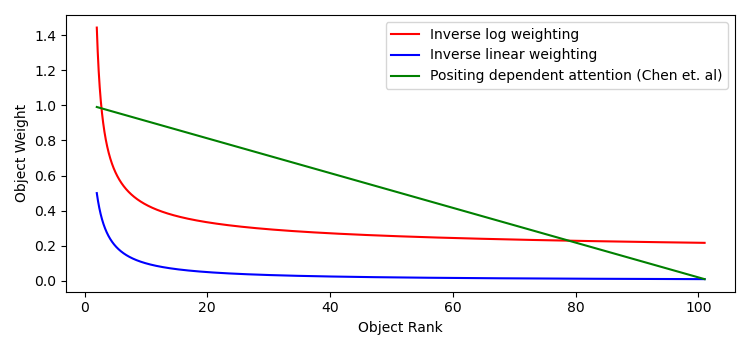
\includegraphics[scale=0.65]{images/weightingfunctions}
    \caption{Different Weighting Functions}
    \label{fig:weightingfunctions}
\end{figure}

Figure~\ref{fig:weightingfunctions} shows all 3 weighting strategies.
In the case of inverse linear strategy,  we see that the weight becomes extremely small after only a few ranks in the list.
This has an unwanted consequence for our problem.
Because the weights of objects at the end of the list are too small,  the ranking function may not learn to rank optimally.

The inverse log weighting was found to be most suitable because it neither completely ignores the objects at the end of the list nor does it given them too high an importance.
In fact,  the weights of the rest of list are very similar which is what we want - all objects at the tail of the list are equally "unimportant" in our case.

Another advantage of using inverse weighting is that we can employ parallelism to enhance our HPO during the optimization cycle.
For example,  at every step the top $n$ configurations can be selected,  and all of them can be tried for optimization.
This overcomes any uncertainties that may occur while ranking the top part of the list. 
The parallelism is less effective when using the weighting proposed by Chen et al.


\iffalse
Applying this to HPOB... (With or without query)
    First learning from first search space.
    Even with this the loss curves are very smooth if we use 2 * tanh(0.01 * x)
\fi
    
\section{Case study with inverse mapping}

In this case study,  we study how the learnt ranking function behaves when we use different parameters to train.
For this a toy example of sorting in the descending order is considered.
    
The main problem that we try to study here is - Is it possible to train a ranking function using the ListMLE loss function such that it learns inverse mapping of points on a number line.
Consider numbers sampled from the range $[k,  p]$ where $k,p > 0$ and  $k,p \in \mathbb{R}$.
If we take 2 numbers $x_1, x_2 \in [k,  p]$,  we need to learn a mapping $s: x \mapsto \mathbb{R}$ such that $s(x_1) \leq s(x_2)$ when $x_1 \geq x_2$.
Consequently we could sort the numbers based on the output of the scorer to obtain a descending sorted order.

Consider a list $l = \{x_1, x_2, ...x_n\}$ where $x_i \in [1, 100]$.
Let $s(x \mid \theta) \mapsto \mathbb{R}$ be our scoring function parametrised by $\theta$.
Here, one list contains $n$ data points sampled from $[1, 100]$.
Then the loss function we would use to learn our scorer is
\begin{equation}
\underset{\theta}{\rm argmin} \quad L_{mle}(s(l \mid \theta),  - k * l)
\end{equation}
where $k \in \mathbb{R}$.
Note that second parameter of list wise loss function is scale invariant hence scaling the list has no effect on the loss output (Section~\ref{sec:listMLE}).

%    #       Result -> Sorting possible provided the output range of the model not restricted
%    #       For now we sample train/val data from the same distribution.
  %  #   List of numbers to test with = {-1 to -100}
%    #       Result -> This is not possible because the model will map this to extreme values as it
 %   #                 is not distribution dependent.
 %   #   Check the percentage of the lists in the correct sorted order.

The validation data taken from 3 different ranges
\begin{itemize}
\item Same range as the training data $[1, 100]$
\item Completely different range as seen by the scorer during training i.e $[-100, -1]$
\item Hybrid range i.e $[-50, 50]$
\end{itemize} 

To evaluate our scorer,  we first sample the validation data from the above ranges,
We then check the percentage of the lists that are correctly sorted during our testing time.
We used the same values of $k$ and $\alpha$ as used in the basic scoring model.
During training a batch size of 100 lists was used.
We try sort 1000 lists according to the learnt scorer's results.
The accuracy gives the fraction of the lists that were sorted in 1000 lists.
We report the average of 5 runs in the Table~\ref{table:caseStudyResults}.

\begin{table} [h!]
\centering
\resizebox{\linewidth}{!} {
\begin{tabular}{ | c | c | c | c | c | c | }
\hline
\textbf{Training Epochs} & \textbf{List size} & \textbf{In-range Acc.} & \textbf{Out-range Acc.} & \textbf{Hybrid Acc.} \\ [0.5 ex]
\hline \hline
1000 & 3 & 0.99 & 0.27 & 0.40\\
100 & 3  & 0.77 & 0.29 & 0.11\\
100 & 30  & 0.80 & 0.79 & 0.46\\
100 & 100  & 0.99 & 0.0 & 0.39\\
1000 & 100  & 1.0 & 0.71 & 0.48\\
\hline
\end{tabular}
}
\caption{Sorting Accuracies at test time}
\label {table:caseStudyResults}
\end{table}

We find from the tabulated results that it is important to completely learn the function by running a higher number of epochs.
To comprehensively learn the scoring function,  it is crucial to have a larger list size.
This will make our scorer model work well when the input is from the same distribution seen during training.
Moreover,  it also gives reasonable when the input comes from the distribution edge (i.e from a location close to the distribution).
These are good properties to have in any machine learning model.

The loss function is not weighted in this toy example because sorting requires that each data point be on its correct location.
Therefore,  our problem is not a direct generalization of this toy example.
Moreover the input domain in the toy example is quite simple as compared to the real world problems.
Nevertheless,  we do take these results into account to decide on the list size for training our proposed ranking surrogate model.

\section{Method training and optimization}

The proposed method in this thesis, "Ranking loss surrogate" is a transfer HPO model.
For this reason its working principle is similar to that of FSBO model.
Like FSBO we use surrogate learning as a knowledge transfer mechanism.
Hence the 2 main parts of using our optimization process are
\begin{itemize}
\item Meta learning the ranking loss surrogate
\item Using the trained surrogate in the evaluation cycle (with or without fine tuning).
\end{itemize}

\subsection{Meta training the surrogate}\label{sec:rlmetatraining}

The space of hyper parameter configurations in which we are trying to get an optimum during any HPO is called HP search space.
This search space is different for different machine learning models.
Hence we need to train different ranking loss surrogate models for different search spaces.

The same machine learning model,  however,  can be used to fit different data sets or tasks.
This leads to different HP response surfaces in the same search space.
Hence,  we obtain different meta data when the same model is optimized on different datasets (or tasks).
The goal of training our model is to use different meta-data sets (or tasks) from a single search space to train our model.
The idea is to learn all the common characteristics of the tasks and transfer this knowledge to the new task.

To train this ensemble, we can employ two strategies:
\begin{itemize}
\item Train each network separately.
\item Use the mean score of the entire architecture to train together.
\end{itemize}
A combined training method may make the training more efficient.
However,  each network's output may affect the training of all other networks.
Moreover, it is absolutely no issue if the outputs of separate DNNs are in different ranges. What matters is the relative rank within a batch.
It is theoretically unnecessary to train the networks together.
The combined training also reduces the variance in the ensemble, which is a disadvantage.
Therefore we train each network separately.

We use stochastic gradient descent to train our model.
For this we need to sample a batch of data from the given meta data.
There are 2 ways to do this:
\begin{itemize}
\item Double sampling: First sample the task then sample the meta data within the task.
\item Sample meta data from all tasks.
\end{itemize}

We use the first method of sampling our data.
This is because due to higher level of sampling,  we have obtain good regularization,
faster training and a possibility to use a lower learning rate.
We use Adam optimizer with a learning rate of 0.001 for our model.
We do our training for 5000 epochs and in each epoch we take 100 steps in which each step does 1 double sampling.
While sampling data points from within a meta data set, we sample without replacement.
We use the number of lists (batch size) as 100 and the size of each list also 100.
Algorithm~\ref{alg:RLSMetaTraining} illustrates us a brief skeleton of our meta training procedure.
After the training,  every model is saved on to a persistent location (e.g. hard disk) so that it can be load when necessary.

\begin{algorithm}[h]
\caption{Ranking Loss surrogate meta training}
\label{alg:RLSMetaTraining}
\hspace*{\algorithmicindent} \textbf{Input} : $epochs \in \mathbb{I}$ \\
 \hspace*{\algorithmicindent} \textbf{Input} : $X_{train}$,  $y_{train}$  \Comment{Meta data used to train} \\
\hspace*{\algorithmicindent} \textbf{Input} : $s_{\theta}$ \Comment{Model to train}
\begin{algorithmic}[1]
\Procedure{MetaTrain}{$s_{\theta}$,  $X_{train}$,  $y_{train}$, $epochs$}
    \For{$i < epochs$}
            \For{$j < 100$}
                \State $B_{X}, B_{y} \gets$ \textsc{DoubleSample}($X_{train}$) \Comment{Get the training batch}
                \State $y_{pred} \gets s_{\theta}(B_{X})$
                \State $\textrm{loss} \gets L_{mle}(y_{pred},  B_{y}) $
                \State $g \gets \frac{\partial \textrm{loss}}{\partial \theta}$ \Comment{$g$ stands for gradient}
                \State Use $g$ to update $\theta$ using the Adam optimizer
            \EndFor
    \EndFor
\EndProcedure
\end{algorithmic}
\end{algorithm}



\subsection{Fine tuning}\label{sec:rlfinetune}
Fine tuning is the second major part of the optimization process.
This may be considered optional for transfer HPO models like ours.
However,  we found that it improved the HPO evaluation cycle performance.

We take the SMBO optimization of Deep Ensembles in Algorithm~\ref{alg:deepEnsembleFinetuning} as an example to understand the fine tuning process.
In this algorithm,  at every evaluation cycle the deep ensembles are retrained with the seen evaluations of the true HPO objective function.
We need to modify Algorithm~\ref{alg:deepEnsembleFinetuning} by replacing Deep Ensemble training with the fine tuning of our model.
The fine tuning  process is exactly similar to the \textsc{MetaTrain} procedure in Algorithm~\ref{alg:RLSMetaTraining}.
The only difference is that we use seen evaluations instead of meta training data for training.
To avoid duplication,  we do not re-write the complete algorithm again.
We do fine tuning for 300 epochs.
The number of epochs can be varied based on the computation resources available.

Like FSBO,  at every evaluation cycle,  the model is reloaded from the saved state before being fine tuned.
In the next section we discuss why this restart is required.
Subsequently we talk about the use of cosine annealing used during fine tuning.

\subsubsection{Requirement of restarting training}\label{sec:restart}

During the implementation of deep ensembles,  we found that the model performs much better in the HPO evaluation cycle when we train it from scratch at every step (acquisition step).
This is counter intuitive because an already trained model should converge to a local optima quickly.
One of the reasons for this performance anomaly is that the model gets biased towards the points that are observed in the starting steps of the optimisation cycle.
Lets say we have 2 models 
\begin{itemize}
\item $\textrm{m}_{\textrm{restart}}$ which always restarts training at every acquisition step.
\item $\textrm{m}_{\textrm{reuse}}$ which trains the model trained in the previous optimization steps.
\end{itemize}

\begin{figure}[h]% [H] is so declass\'e!
\centering
\begin{minipage}{0.45\textwidth}
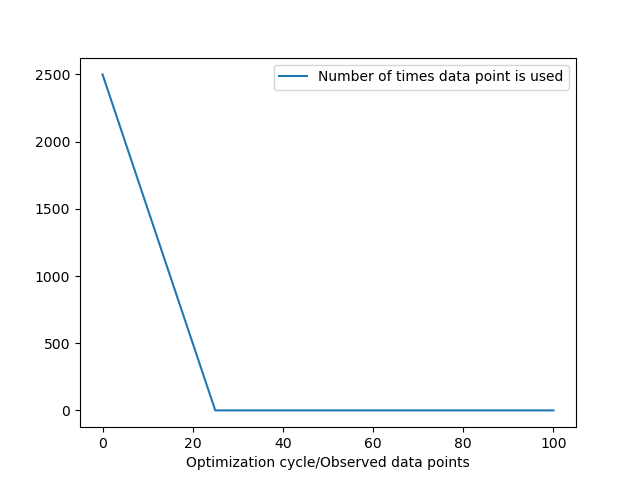
\includegraphics[width=\textwidth]{images/bias25}
\caption{Bias at 25th optimization cycle}
    \label{fig:bias25}
\end{minipage}\hfill
\begin{minipage}{0.45\textwidth}
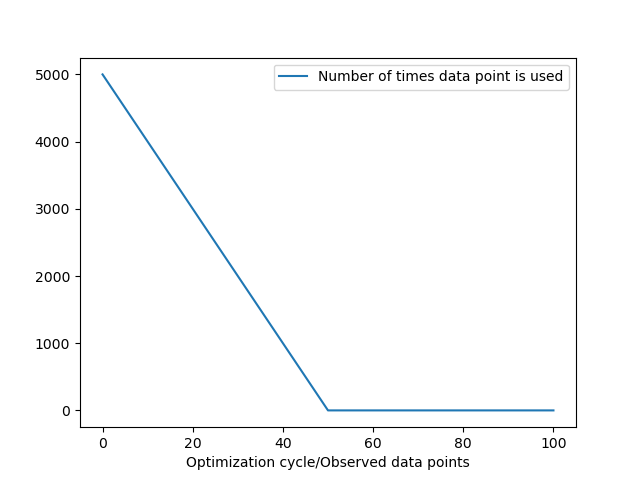
\includegraphics[width=\textwidth]{images/bias50}
\caption{Bias at 50th optimization cycle}
    \label{fig:bias50}
\end{minipage}\par
\vskip\floatsep% normal separation between figures
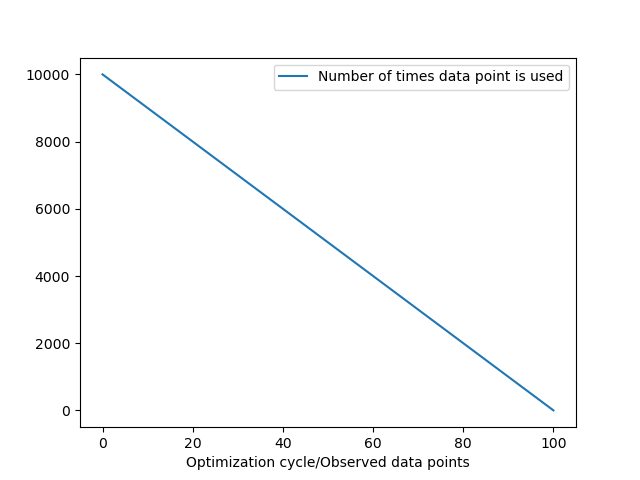
\includegraphics[width=0.45\textwidth]{images/bias100}
\caption{Bias at 100th optimization cycle}
    \label{fig:bias100}
\end{figure}


Let the models be fine tuned for 100 epochs at each step.
Let there be just 1 seen HP configuration to start with.
The figures~\ref{fig:bias25},~\ref{fig:bias50},  and ~\ref{fig:bias100} show the number of times each observed HP configuration is used for training the model at the 25th, 50th and 100th optimization cycle step by the $\textrm{m}_{\textrm{reuse}}$ model.

Generally all the data is used during fine tuning due to data scarcity.
Hence,  in our example the number of times an HP configuration is used scales with the number of epochs trained.
The heavy bias that is present in the figures is actually not intended.
This is because all observations should be treated equally in any training/fine-tuning step.
When we use $\textrm{m}_{\textrm{restart}}$ every known HP configuration is used only 100 times at every evaluation step.
Hence it is better to restart the model before fine tuning.

The second reason for restarting is that the model may get stuck at a stubborn local minima at any fine tuning step $n$ where $1 <= n <= 100$ in our case.
Coming out of this local minima may require the response surface to change very drastically.
The response will change like this only when the training data distribution significantly changes.
This is not possible in the sequential process of SMBO because at every step only 1 new HP configuration is added to the known HP configurations.

\begin{figure}[htb]
  \centering
    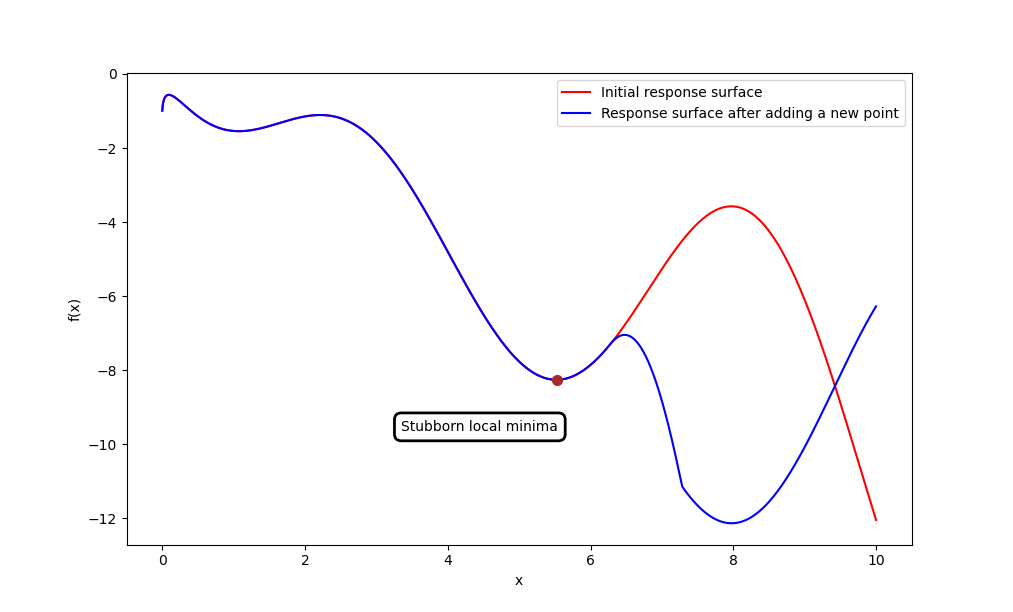
\includegraphics[scale=0.45]{images/localMinima}
    \caption{Figure showing changes in response surfaces and a stubborn local minima}
    \label{fig:localMinima}
\end{figure}

Figure~\ref{fig:localMinima} depicts this issue for a simple 1 dimensional case.
Consider the red curve.
It represents the HP response surface for $k$ known data points.
When we add $(k+1)^{th}$ data point,  most of the response surface remains the same.
Only part of it changes.
This is represented by the blue response surface.
If our model is already trained for the red curve,  it becomes extremely difficult for it to come out of local minima because of the minimal changes in the response surface.
We call this minima a stubborn local minima.
This is depicted by the brown dot in the figure.

If however,  we reload and retrain our model from the beginning there is more chance of it reaching the good local optima in the blue curve if it descends from the other direction.
The number of ways to reach a good local minima increases exponentially with the increase in the HP search space dimensions.
Hence, restarting the training (from the saved model in our case) should improve our fine tuned model.

Because of these reasons,  we use the restart mechanism during the fine tuning of our ranking loss model (and also baseline implementations).
This makes the model more robust.

\subsubsection{Using cosine annealing}

We plotted the fine tuning loss curves of our model
We found that these loss curves were very jittery.
We noticed the same behaviour when fine tuning FSBO model.
Figure~\ref{fig:jitteryFTLoss} shows the fine tuning loss for one of the search spaces.

\begin{figure}[htb]
  \centering
    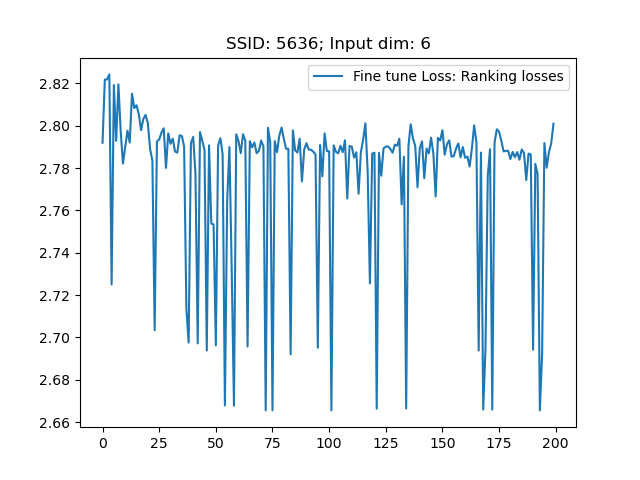
\includegraphics[scale=0.45]{images/jitteryFTLoss}
    \caption{Figure showing jittery loss function curve}
    \label{fig:jitteryFTLoss}
\end{figure}

We hypothesise that these jittery losses are because the learning rate is not suitable with the response curve's curvature at the targeted local minima.
One solution to this is to use a smaller learning rate.
However,  the fine tuning using smaller learning rate will take a long time.
The solution we proposed and utilized was using cosine annealing.

There are couple of advantages of using cosine annealing.
First the initial learning rate is kept high in order to give the optimizer time to get to an area close to the local minima if it has not done so.
Thereafter,  the learning rate declines quickly to the target small learning rate.
This helps the model to get deep into the local minima and hence the possibility of the optimization to jump out of the local minima is very less.

\begin{figure}[htb]
  \centering
    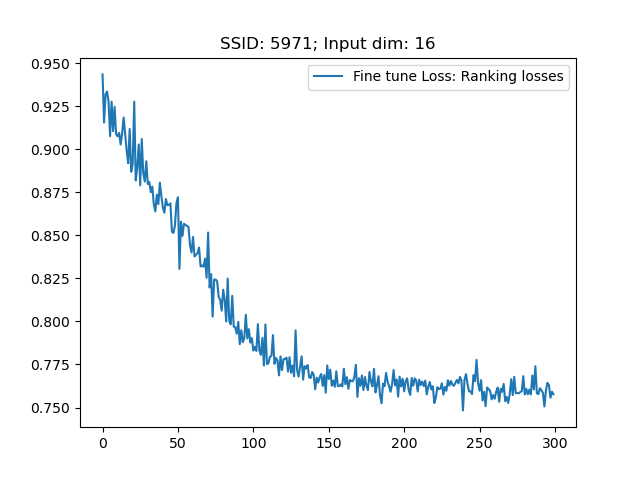
\includegraphics[scale=0.45]{images/goodFTLoss}
    \caption{Figure showing a loss curve obtained by using cosine annealing}
    \label{fig:goodFTLoss}
\end{figure}

Figure~\ref{fig:goodFTLoss} shows a fine tuning loss curve obtained using cosine annealing.
Even though this strategy may not be a perfect one,  it reduces the possible problems that could prop us when using a constant learning rate.
During training,  however,  we use a constant learning rate as can use the validation loss as a reference for over fitting or under fitting.

\section{Ranking Surrogate Model}

After explaining the learning mechanism,  we now turn to 2 important components that are used in our method.
The first is Deep Set to make our model context aware.
The second is the use of uncertainty for improving the output of the model.

\subsection{Using Deep Sets to build context aware models}\label{sec:DeepSetWithModel}

We have already discussed the fundamental ideas of using deep sets in  ~\ref{sec:DeepSets}.
In this section we discuss about how to add deep sets in the ranking loss surrogate model architecture and then how to train the same.

The basic idea is to precondition our scoring function $s_{\theta}$ on known evaluations of the target HP space.
These known evaluations act as a support for the scoring function.
Hence they are subscripted as "s" in the equation.
We then query the scoring function to get the relevant scores of new $\textbf{X}$ which are subscripted as "q" in the equation.
The scoring function hence becomes:
$$
s_{\theta}(\textbf{X}_{q} | \textbf{X}_{s}, \textbf{y}_{s})
$$

\begin{figure}[htb]
\centering
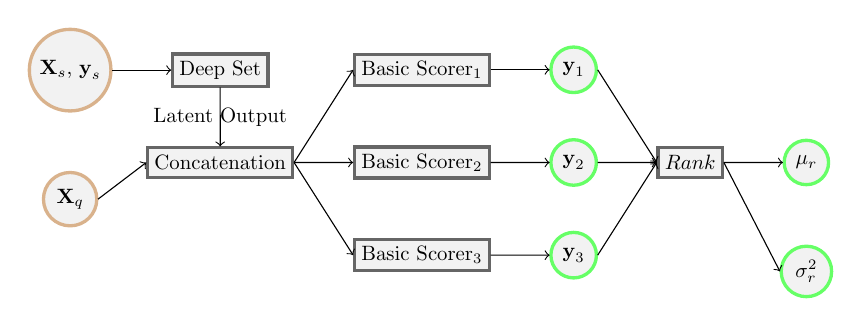
\begin{tikzpicture}[scale=0.75, transform shape,
roundnode/.style={circle, draw=brown!60, fill=black!5, very thick, minimum size=7mm},
roundnodey/.style={circle, draw=green!60, fill=black!5, very thick, minimum size=7mm},
squarednode/.style={rectangle, draw=black!60, fill=black!5, very thick, minimum size=5mm},
]
%Nodes
\node[roundnode]          (Xs)                                                     {$\textbf{X}_s$, $\textbf{y}_s$};
\node[roundnode]          (Xq)                        [below=of Xs]     {$\textbf{X}_q$};
\node[squarednode]      (DeepSet)              [right=of Xs]        {Deep Set};
\node[squarednode]      (Concatenation)             [below=of DeepSet]        {Concatenation};
\node[squarednode]      (DNN2)                      [right=of Concatenation]        {Basic Scorer$_2$};
\node[squarednode]      (DNN1)                      [above=of DNN2]                    {Basic Scorer$_1$};
\node[squarednode]      (DNN3)                      [below=of DNN2]                    {Basic Scorer$_3$};
\node[roundnodey]        (y1)                             [right=of DNN1] {$\textbf{y}_1$};
\node[roundnodey]        (y2)                             [right=of DNN2] {$\textbf{y}_2$};
\node[roundnodey]        (y3)                             [right=of DNN3] {$\textbf{y}_3$};
\node[squarednode]      (mean)                             [right=of y2] {$Rank$};
\node[roundnodey]        (mus)                             [right=of mean] {$\mu_r$};
\node[roundnodey]        (sigmas)                             [below=of mus] {$\sigma^2_r$};

%Lines
\draw[->] (Xs.east) -- (DeepSet.west);
\draw[->] (DeepSet.south) -- (Concatenation.north) node[midway] {Latent Output};
\draw[->] (Xq.east) -- (Concatenation.west);
\draw[->] (Concatenation.east) -- (DNN1.west);
\draw[->] (Concatenation.east) -- (DNN2.west);
\draw[->] (Concatenation.east) -- (DNN3.west);
\draw[->] (DNN1.east) -- (y1.west);
\draw[->] (DNN2.east) -- (y2.west);
\draw[->] (DNN3.east) -- (y3.west);
\draw[->] (y1.east) -- (mean.west);
\draw[->] (y2.east) -- (mean.west);
\draw[->] (y3.east) -- (mean.west);
\draw[->] (mean.east) -- (mus.west);
\draw[->] (mean.east) -- (sigmas.west);

\end{tikzpicture}
\caption{Skeleton of the proposed model with Deep Sets.}
\label{fig:proposeModelDeepSets}
\end{figure}

The  architecture of the scoring function $s_{\theta}$ with deep sets is given in Figure~\ref{fig:proposeModelDeepSets}.
For the complete architecture of the Deep Set node please refer~\ref{fig:DeepSetArchitecture}.
We keep the node abstract for simplicity.\

First the data points in the query set $\textbf{X}_q$, $\textbf{y}_q$ are passed through the deep set to get the Latent Output.
Each $X$, $y$ are concatenated to get a single vector for input into the deep set.
We obtain a latent output from the deep set.
This latent output is then concatenated with the query data points.
The concatenated result is passed through a Deep Neural Network to finally get the desired relevance scores.
For example if there is a batch of queries given by $\{X_{q_1},  X_{q_2},  X_{q_3} ...\}$,  and the latent output is given by $O_l$ then the concatenation yields
$$
\{O_l:X_{q_1},  O_l:X_{q_2},  O_l:X_{q_3} ...\}
$$
where ":" represents concatenation of 2 vectors.

\subsubsection{Meta training}

Using the above given scoring function during the evaluation cycle is very straightforward.
We use the known data points as a support set and the target data points to evaluate as the query set.
During meta training,  however,  we have to divide the training data into support set and query set.

In our data division we first select 20 ($X$, $y$) data points as a support set randomly without replacement.
Thereafter,  we select the query points from the remaining choices (again without replacement). The number of query points depends on the batch size (100 by default).
During the meta training we do not sample the support and query points from all the given meta datasets.
At each step within an epoch we select one meta data to sample these points as discussed in Section~\ref{sec:rlmetatraining}.
For the purpose of analysing the training progress accurately,  we however sample data from all the training and validation task to report the complete training and validation loss respectively.



\iffalse
\chapter{Research Question}
The format of this is the same as that of experiments and Results.
Also known as Hypothesis.
\fi

\chapter{Experiments and Results}

In this chapter, we present the experiments we conducted and the results we obtained to some of the research questions that arose during the thesis.
We first understand the structure of the metadata used for meta-training,  meta-validation,  and meta-testing.
In the subsequent sections, we present the results obtained in detail.

\subsubsection{Meta-Data}

To compare our proposed ranking loss surrogate with other HPO surrogates, we would have to run the Bayesian optimization (BO) on a set of different machine learning models.
The BO would have to be run with the ranking loss surrogate and other surrogates.
Moreover, the optimum within the HP search space is different when the ML model is trained on different data sets.
In addition to this, due to the stochastic nature of ML models and the surrogate models, we would have to run the HPO multiple times for each dataset.

As one can see,  this evaluation, if done right from the training of the ML models, is not feasible.
To overcome this challenge, we use a meta dataset proposed by Pineda
 et al. called HPO-B~\cite{DBLP:journals/corr/abs-2106-06257} to benchmark our results in the thesis.
Using this benchmark, we do not need to train our ML models from scratch, as the metadata contains evaluations of multiple HP configurations for different ML models and datasets.
In the rest of the section, we discuss the organization of the benchmarking metadata.

HPO-B is a benchmark that is used for doing black box HPO.
Both transfer and non-transfer HPO surrogates can be studied using this benchmark.
The meta data in HPO-B comes in 3 versions namely \textbf{HPO-B-v1},  \textbf{HPO-B-v2}, and \textbf{HPO-B-v3}.
Of this \textbf{HPO-B-v3} contains distilled search spaces that have the most datasets. \textbf{HPO-B-v3} can be split into meta-training, meta-validation, and meta-test sets. 
Using the meta-training dataset, one can meta-learn an HPO surrogate.
Then the surrogate is evaluated and tested using the meta-validation and meta-test data, respectively.
The metadata in any split (training, testing, or validation) is organized in a JSON format. Figure~\ref{fig:metadataorganization} shows an illustration of this format.

\begin{figure}[htb]
\centering
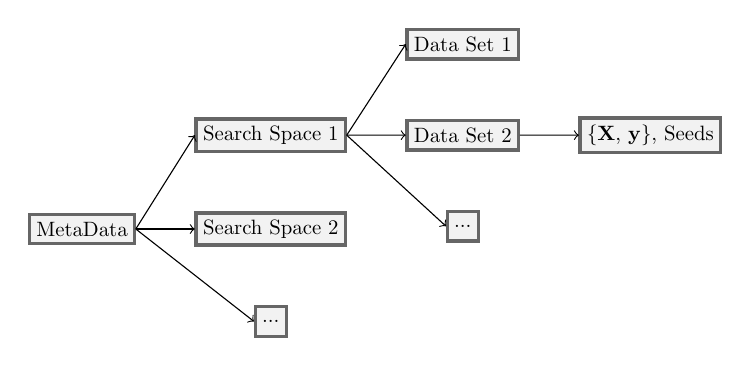
\begin{tikzpicture}[scale=0.75, transform shape,
% roundnode/.style={circle, draw=green!60, fill=green!5, very thick, minimum size=7mm},
squarednode/.style={rectangle, draw=black!60, fill=black!5, very thick, minimum size=5mm},
]
%Nodes
\node[squarednode]      (ss2)                             {Search Space 2};
\node[squarednode]      (main)                   [left=of ss2]           {MetaData};
\node[squarednode]      (ss1)                    [above=of ss2]          {Search Space 1};
\node[squarednode]      (ss_)                       [below=of ss2]        {...};
\node[squarednode]      (ds2)                       [right=of ss1]        {Data Set 2};
\node[squarednode]      (ds1)                       [above=of ds2]        {Data Set 1};
\node[squarednode]      (ds_)                       [below=of ds2]        {...};
\node[squarednode]      (Xy)                       [right=of ds2]        {\{\textbf{X},  \textbf{y}\},  \textrm{Seeds}};

%Lines
\draw[->] (main.east) -- (ss2.west);
\draw[->] (main.east) -- (ss1.west);
\draw[->] (main.east) -- (ss_.west);
\draw[->] (ss1.east) -- (ds2.west);
\draw[->] (ss1.east) -- (ds1.west);
\draw[->] (ss1.east) -- (ds_.west);
\draw[->] (ds2.east) -- (Xy.west);
\end{tikzpicture}
\caption{Structure of the metadata in the HPO-B benchmark.}
\label{fig:metadataorganization}
\end{figure}

As shown in Figure~\ref{fig:metadataorganization}, the metadata consists of a list of HP search space ids. An HP search space id corresponds to a single ML model. Each search space further has multiple dataset ids.
These dataset ids correspond to different training data used to train ML models. Each dataset id contains an \textbf{X}, \textbf{y} pair and 5 seeds. \textbf{X} represents a set of HP configurations and
\textbf{y} represents their respective true evaluations. The Bayesian optimization used in our thesis starts with different initial known HP configurations. One initial configuration is called a seed. A seed gives a set of values (or indices in implementation) from the $\textbf{X}$,  $\textbf{y}$ pair.

We compare the results of ranking loss surrogates with transfer HPO surrogates and non-transfer HPO.
HPO-B can be used for analyzing both types of surrogates.
However, to cross-compare transfer and non-transfer HPO,  we only compare against \textbf{HPO-B-v3} test split as recommended by Pineda
 et al. ~\cite{DBLP:journals/corr/abs-2106-06257}.


\iffalse
\subsection{HPO-B Dataset}
To use the HPO-B code,  one must write function observe\_and\_suggest and observe\_and\_suggest\_continous to deal with discrete and continous optimisation case respectively.
Due to out of scope nature of the continous case,  in our implementation we assume that we are dealing only with the discrete case only.

The implementation of observe\_and\_suggest functions differs based on the surrogate model used by our problem.
\fi

\subsubsection{Experimental Protocol}
To test the performance of ranking loss surrogates at different stages of development, we used four main baseline methods - Random Search,  SMBO using a Gaussian surrogate, SMBO using Deep Ensembles, and FSBO.
We reused the Gaussian and Random surrogate implementations of HPO-B in the thesis.
However, the Deep Ensemble and FSBO surrogates were implemented from scratch.

In the given meta data if we take the set of all combinations in \textbf{HPO-B-v3} test split i.e \{Search Spaces $\times$ Metadata sets $\times$ Seeds\}, we get 430 HP optimizations.
We start with five initially known HP configurations given by the HPO-B seed in each optimization and run the evaluation cycle for 100 iterations.
This evaluation cycle is discussed in Algorithm~\ref{alg:deepEnsembleFinetuning} albeit for deep ensembles.

One optimization creates one array of incumbent best (highest) HP evaluations.
This incumbent array for different models is compared against each other to create a rank array for each surrogate.
For example, if at the evaluation step 23, the incumbent of surrogate $a$ has a higher value than of surrogate $b$, then the rank of model $a$ at step 23 is lower than model $b$ (if we consider lower rank to be better).
We get a list of rank arrays for every surrogate if we do this for all optimizations.
This rank array list is averaged to get a single averaged rank array.
Plotting this averaged rank array gives us a rank graph of a surrogate.
We use this \textbf{rank graph} to compare the different surrogates in this thesis.
For example, Figure~\ref{fig:RsGpRankGraph} compares the rank graph of 2 baselines.

\section{Baseline Results}
The results of Deep Ensemble and FSBO baselines are discussed in this section.

\begin{figure}[htb]
  \centering
    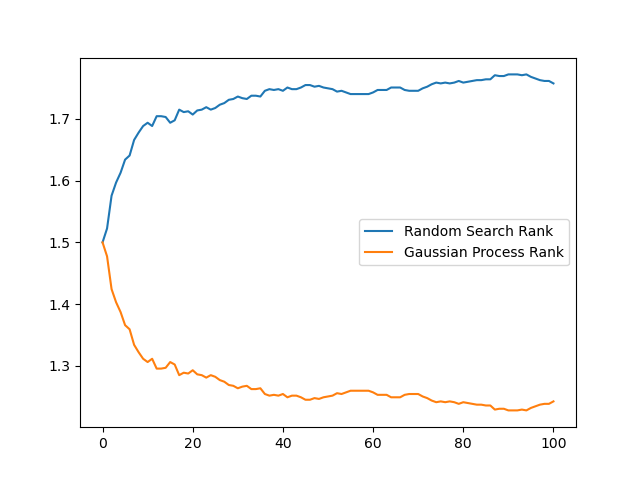
\includegraphics[scale=0.5]{images/RsGpRankGraph}
    \caption{Sample rank graphs of Random and Gaussian surrogates.}
    \label{fig:RsGpRankGraph}
\end{figure}

\subsubsection{Deep Ensembles}

The deep ensembles we used contained five neural networks by default. Each neural network had two fully connected neural layers with 32 neurons each. We considered the non-transfer case for deep ensembles first. Hence we did not do any meta training for this model.
We train each neural network for 1000 epochs with a learning rate of 0.02 at every evaluation step in an HPO optimization. We used Adam as our optimizer.

\begin{figure}[h]
  \centering
    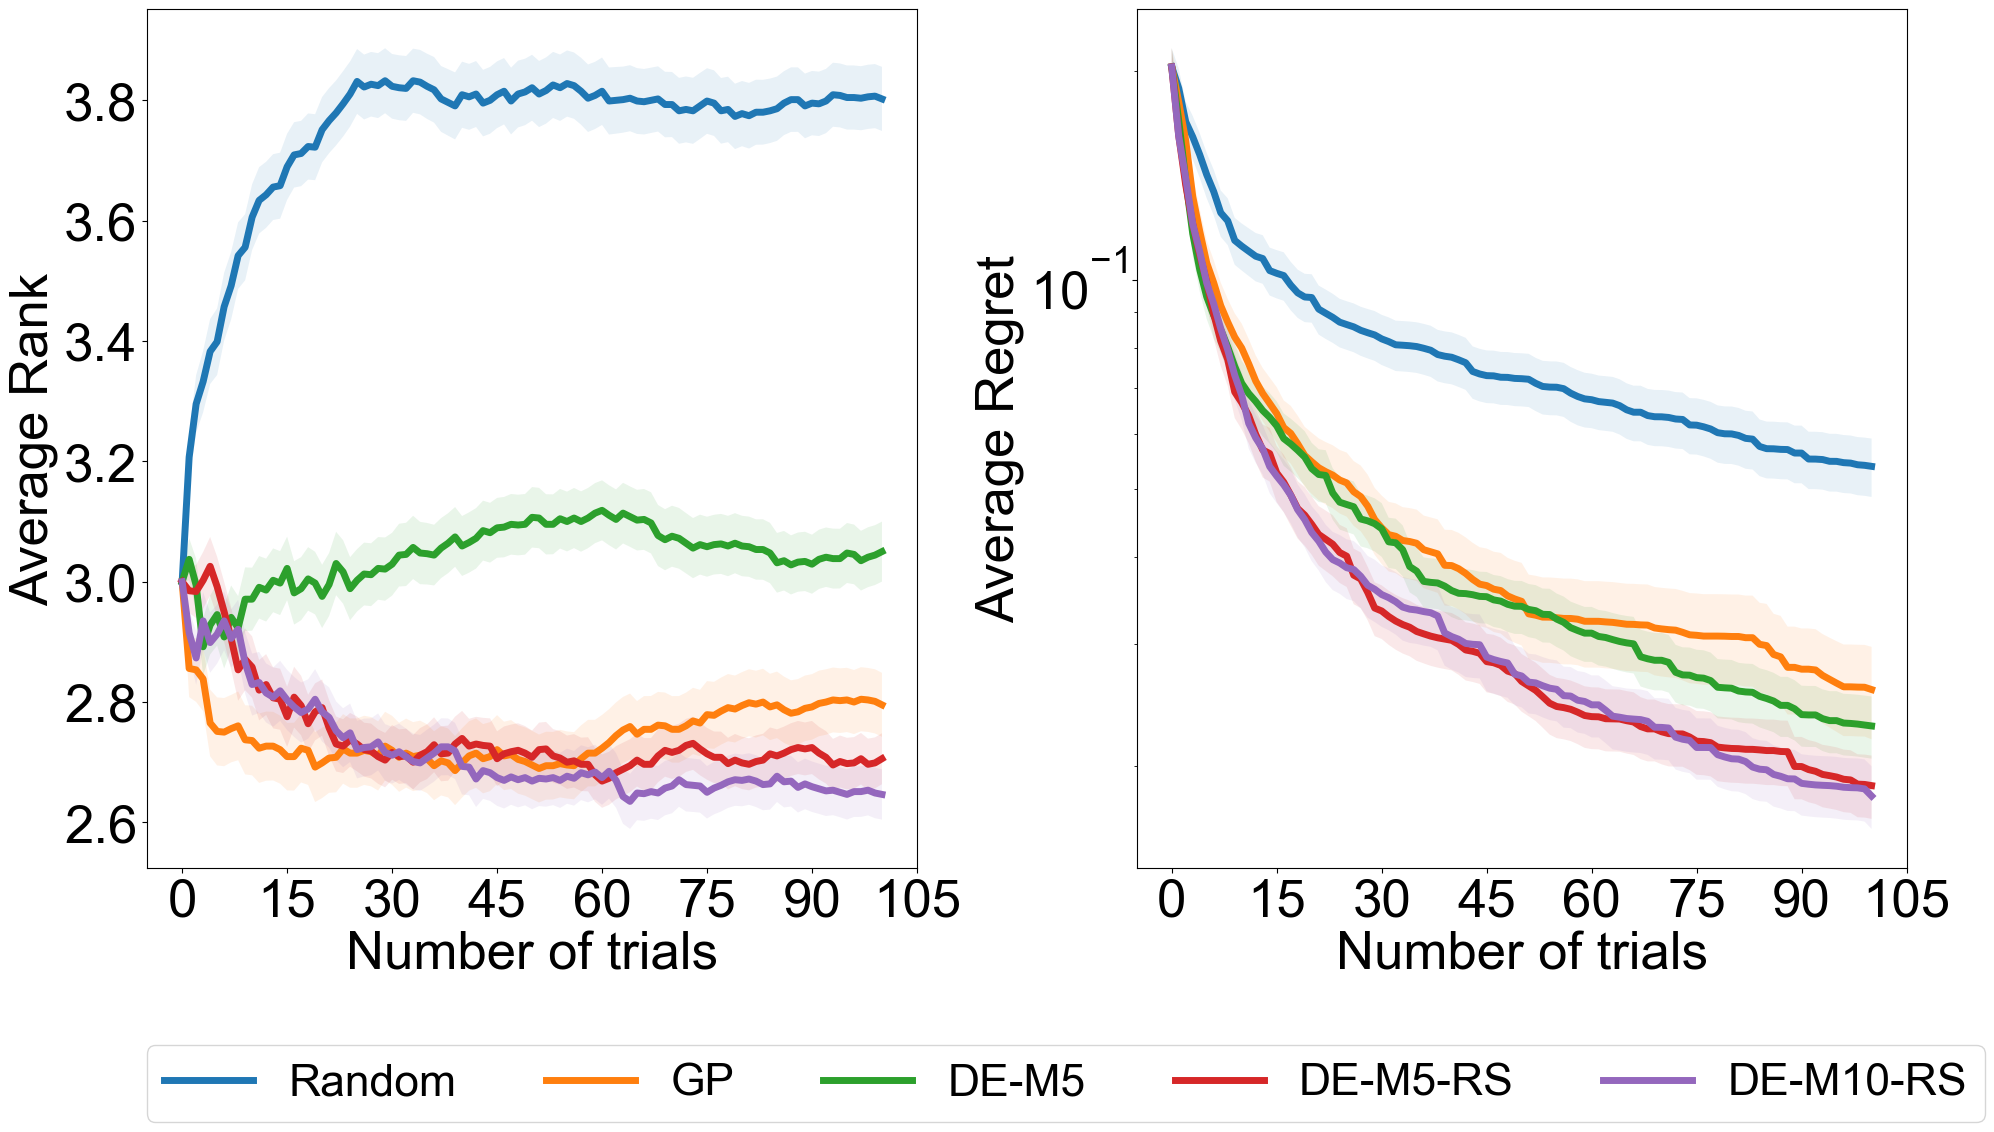
\includegraphics[scale=0.25]{images/DEPerformance}
    \caption{Graphs showing performance of Deep Ensembles.}
    \label{fig:DEPerformance}
\end{figure}

Figure~\ref{fig:DEPerformance} shows the performance of various Deep Ensemble models.
We used the best results of Random and Gaussian surrogate baselines to compare how Deep ensembles fair in the HPO-B benchmark.
In addition to plotting the rank graph,  we also plot the average regret for every model.
In the average regret graph, the y-axis represents the regret on a log scale.
In Figure~\ref{fig:DEPerformance},  DE\_M5 stands for Deep Ensembles with five neural networks, whereas DE\_M10 stands for Deep Ensembles with ten neural networks.
An "rs" suffix in the legend denotes that the surrogates are reinitialized before fine-tuning at every evaluation step.

In this thesis, we studied the following main models of Deep Ensembles
\begin{itemize}
\item Deep Ensembles that fine-tune with no restarting.
\item Deep Ensembles that fine-tune with restart at every evaluation step.
\item Deep Ensembles with 5 and 10 neural networks.
\end{itemize}

We observed in our study that Deep Ensembles with restarts (at every evaluation step) give us better results than Deep Ensembles that do not do a restart.
This observation proves our hypothesis of the requirement of restarts as discussed in Section~\ref{sec:restart}.
Furthermore,  we observe that using deep ensembles with restarts gives us results comparable with Gaussian surrogates.
Increasing the number of neural network ensembles does not improve performance significantly.
We see this illustrated both in the ranking graph and the average regret graph.
We also use critical rank graphs developed by Pineda et al. ~\cite{pineda2021hpob}.
Critical graphs represent ranks at particular evaluation steps averaged across all HPO optimizations. 
Figure~\ref{fig:DERank100} illustrates a critical rank graph for the Deep Ensemble study.

\begin{figure}[h]% [H] is so declass\'e!
\centering
\begin{minipage}{0.45\textwidth}
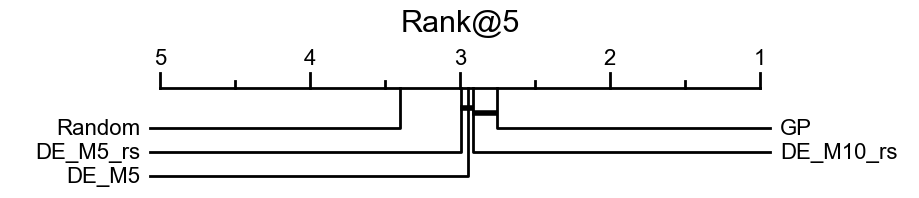
\includegraphics[width=\textwidth]{images/DERank5}
\end{minipage}\hfill
\begin{minipage}{0.45\textwidth}
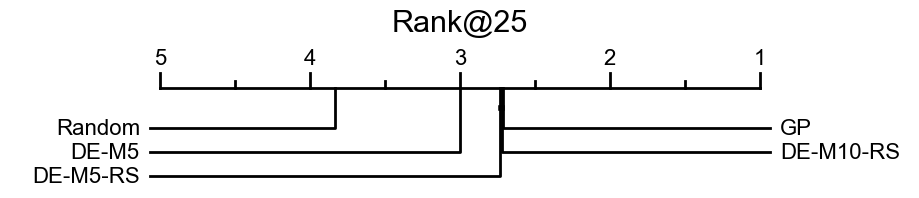
\includegraphics[width=\textwidth]{images/DERank25}
\end{minipage}\par
\begin{minipage}{0.45\textwidth}
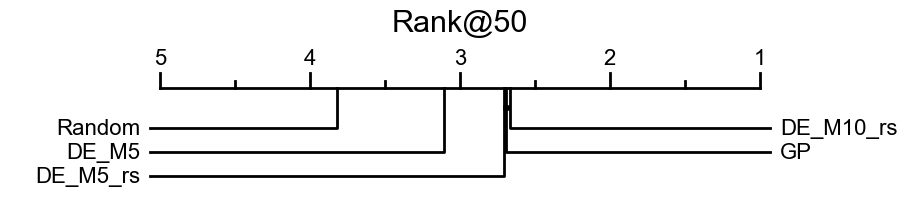
\includegraphics[width=\textwidth]{images/DERank50}
\end{minipage}\hfill
\begin{minipage}{0.45\textwidth}
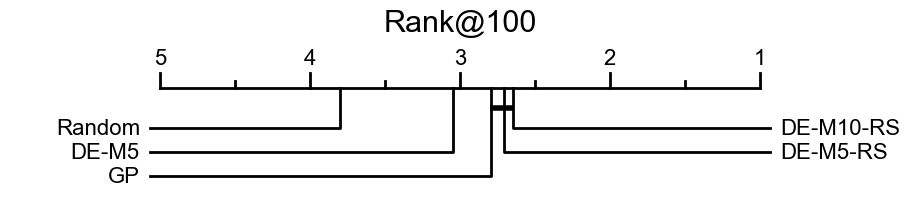
\includegraphics[width=\textwidth]{images/DERank100}
\end{minipage}
% \vskip\floatsep% normal separation between figures
    \caption{Critical rank graphs of Deep Ensembles at the $5^{th}$, $25^{th}$, $50^{th}$, and $100^{th}$ evaluation step.}
   \label{fig:DERank100}
\end{figure}

After the DE results analysis, several advantages and disadvantages of using the DE surrogate were found.
First, being a non-transfer HPO surrogate, DE can be applied to any continuous HPO problem.
Second,  as each neural network is independent of the others,  the neural networks can be trained in parallel.
Hence, DE can be scaled quickly based on the available computing power.
On the negative side,  since no meta-training is done, we have to fit the DE on the very few data points available during the HPO optimization.
This training on very few data points leads to overfitting DE surrogates because of their enormous representative capacity.
In addition, DE is incapable of modeling objective functions with discrete or semi-discrete domains.
The input data points to DE are assumed to lie in a continuous space.
Hence DE will not be able to model discrete and semi-discrete HP search space trivially.


\subsubsection{Few Shot Bayesian Optimization (FSBO)}

FSBO was selected as a baseline because it was the state-of-the-art baseline in the transfer HPO problem domain.
During our implementation of FSBO, we found that an FSBO model with four neural network layers of 32 neurons each gave us the best performance.
This architecture is similar to the Deep Ensemble architecture.
The difference between the architectures is that FSBO has four network layers instead of 2.
We used early stopping to get better training loss, as mentioned in Section~\ref{sec:FSBOBackground}.
During the finetuning, we trained our model for 500 epochs with a learning rate of 0.03.
We used Adam optimizer for both training and finetuning.
The only significant difference between the training and finetuning phase was that we used cosine annealing in the finetuning phase. The reason for using cosine annealing has been discussed in Section~\ref{sec:rlfinetune}.
Finally, we also do restarts for the FSBO domain with the restart mechanism discussed in Section~\ref{sec:FSBOBackground}.

\begin{figure}[h]
  \centering
    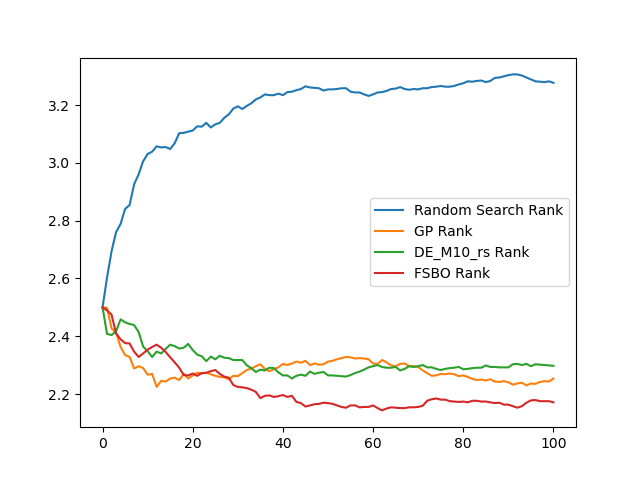
\includegraphics[scale=0.5]{images/FSBOPerformance}
    \caption{Rank graph showing performance of self implemented FSBO.}
    \label{fig:FSBOPerformance}
\end{figure}

Figure~\ref{fig:FSBOPerformance} shows the rank graph of FSBO compared to the best performing models of random search, GP and DE surrogates.
There is a slight difference in ranking graphs of previous surrogates because a few HPO optimizations were unsuccessful for the FSBO due to non-positive definite Matrix exceptions obtained during meta-training and fine-tuning (The GPytorch implementation threw this).
As we can see,  our implementation could not give us state-of-the-art results for FSBO.
Since these results are a correct yardstick to measure the ranking loss surrogate model, we used the results obtained by the FSBO implementation provided by Pineda et al. ~\cite{pineda2021hpob} in the rest of the thesis.


Figure~\ref{fig:FSBOBestPerformance} compares the best performing FSBO surrogate against the performance of other baseline surrogates.
As one can see from this figure, FSBO is an HPO model that outperforms the other HPO models both in the rank graph and the regret graph.
Moreover,  FSBO always has a better rank at every evaluation step.
This can be seen in the critical rank graphs illustrated in Figure~\ref{fig:FSBOBestPerformanceRank100}.
Using these baseline results as a reference, we discuss how the ranking loss surrogate model compares to these methods in detail in the following sections.

\begin{figure}[h]
  \centering
    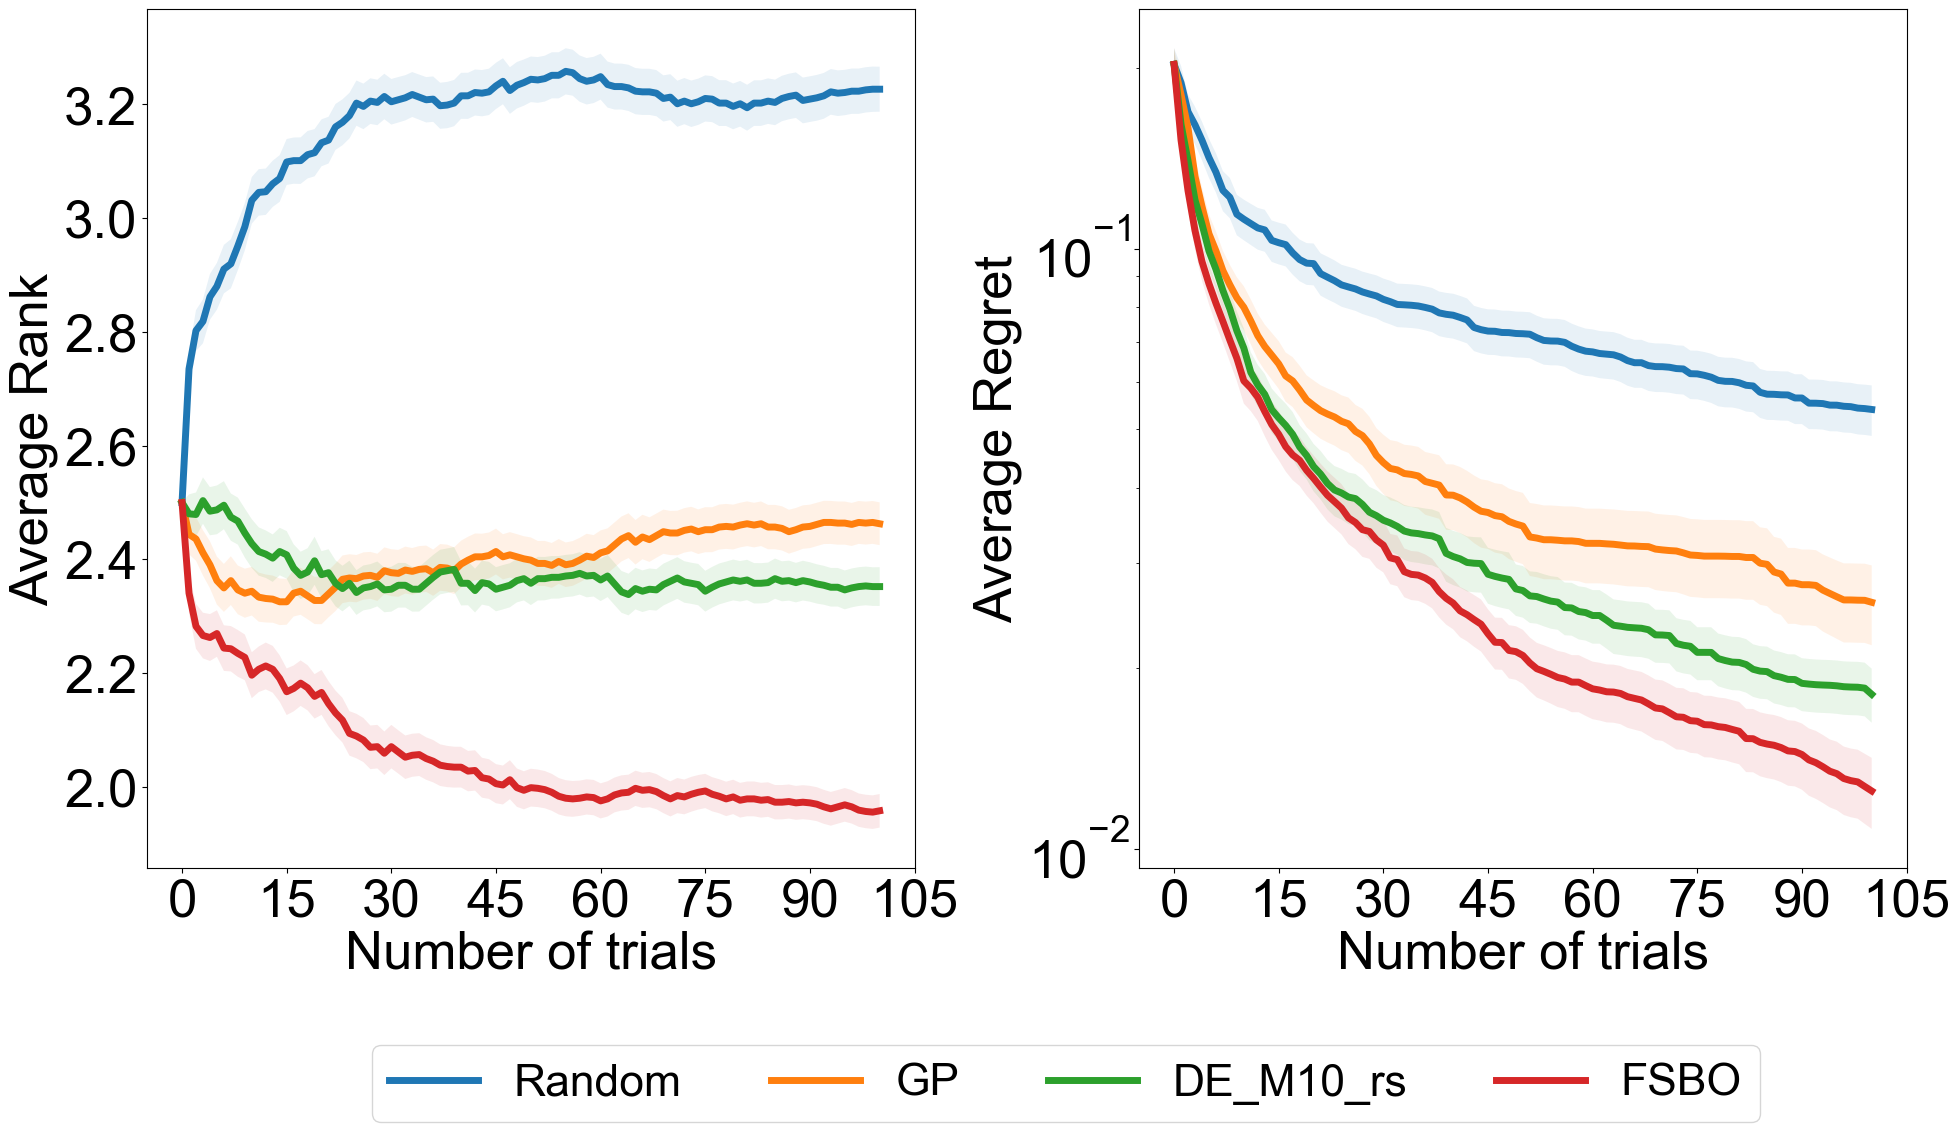
\includegraphics[scale=0.25]{images/FSBOBestPerformance}
    \caption{Rank and regret graph of best performing of FSBO.}
    \label{fig:FSBOBestPerformance}
\end{figure}


\begin{figure}[h]% [H] is so declass\'e!
\centering
\begin{minipage}{0.45\textwidth}
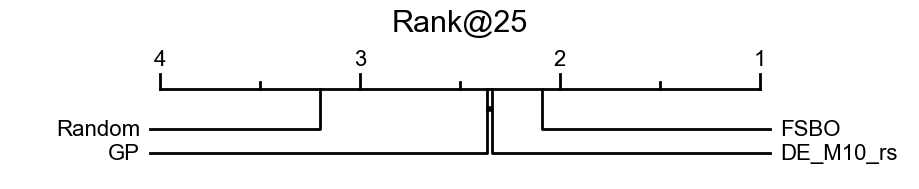
\includegraphics[width=\textwidth]{images/FSBOBestPerformanceRank25}
\end{minipage}\hfill
\begin{minipage}{0.45\textwidth}
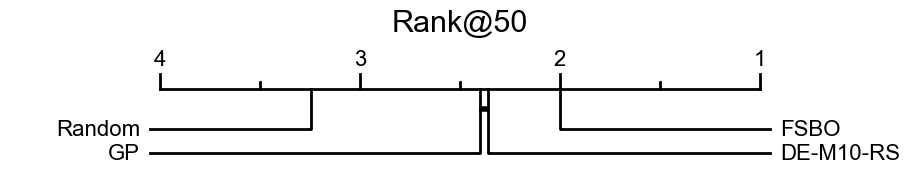
\includegraphics[width=\textwidth]{images/FSBOBestPerformanceRank50}
\end{minipage}\par
\vskip\floatsep% normal separation between figures
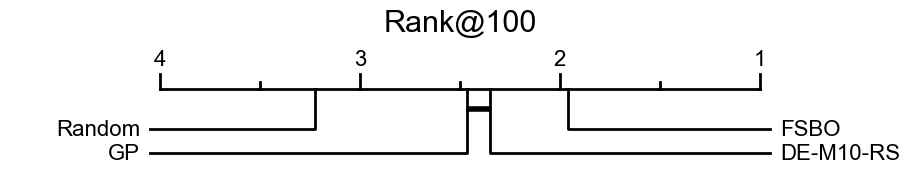
\includegraphics[width=0.45\textwidth]{images/FSBOBestPerformanceRank100}
    \caption{Critical rank graphs of baselines at different evaluation steps.}
   \label{fig:FSBOBestPerformanceRank100}
\end{figure}

\section{Ranking Loss model results: Research question results}

As discussed in Chapter~\ref{chap:ProposedIdea},  our proposed idea has two components - a ranking loss and a surrogate model.
In both these components, several research questions need to be studied.
This section discusses the results or answers to these research questions in different sub-sections separately.
In each section, we present an ablation study to highlight the essential components of our proposed idea.

For uniformity, we use the following strategy - We will use the same number of neural networks and the same neural network architecture in our study.
We also try to keep the learning rate similar for similar components.
For different components, however, we use different learning rates.
For example, learning rates during meta-training and fine-tuning are different.
Similarly, each loss function may require a different learning rate to perform the best as the HP response surfaces change with the used loss function.
Like in the best case of Deep Ensembles, we use ten neural networks in our ensemble. Each neural network has two 32-neuron layers.

\subsection{Meta training results}
In this section, we discuss the observations we made during the meta-training of the proposed model. The effect of finetuning on the optimization results is discussed in detail in Section~\ref{sec:EffectOfFineTuningResults}. Please note that this meta-training is required only for the transfer HPO case. For the non-transfer case, we directly do a finetuning with the evaluated HP configurations during the HP optimization.
The two main architectures we study in this thesis are the Basic Scoring model and the Basic Scoring model with Deep Sets. 

The training of the Basic Scoring Model (without Deep sets) obtained relatively smooth loss curves. This is illustrated using the loss curves of the search space with id "4796" in Figure~\ref{fig:loss4796BasicScoringModel}. The "input dim = 3" in the image title specifies that the dimensionality of this HP search space is 3. After adding deep sets to the model, the loss curves become jumpy. This is illustrated in Figure~\ref{fig:loss4796DeepSets} using the same search space. These jumpy loss curves are expected because adding deep sets increases the architecture's representation capacity (and the parameter space). A bigger parameter space results in more noisy gradients during the stochastic gradient descent. 

\begin{figure}[h]% [H] is so declass\'e!
\centering
\begin{minipage}{0.45\textwidth}
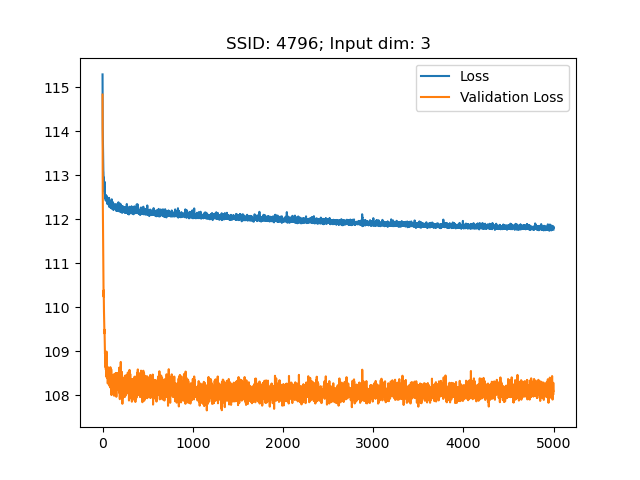
\includegraphics[width=\textwidth]{images/loss4796BasicScoringModel}
\caption{Loss curves for the basic scoring model.}
    \label{fig:loss4796BasicScoringModel}
\end{minipage}\hfill
\begin{minipage}{0.45\textwidth}
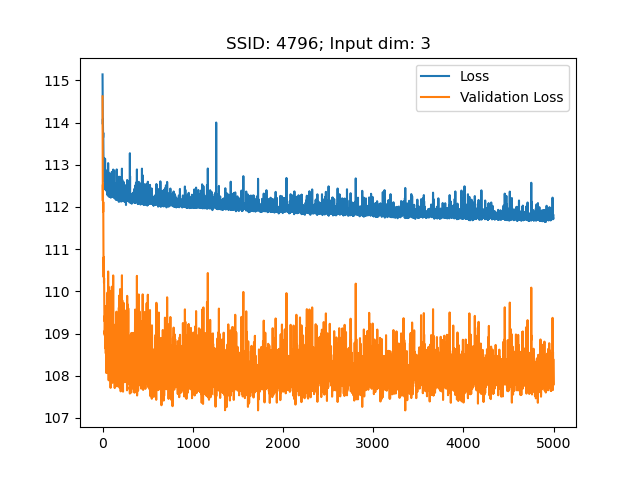
\includegraphics[width=\textwidth]{images/loss4796DeepSets}
\caption{Loss curves for a model with deep sets.}
    \label{fig:loss4796DeepSets}
\end{minipage}
\end{figure}

The second thing we observed is that sometimes the validation loss gets significantly worse during the training. Figure~\ref{fig:NegativeTransferLearning} illustrates this sort of behavior. One reason for this behavior could be that the validation task is not similar to the training task.
There is some negative knowledge transfer from the meta-training phase to the meta-validation phase. This type of learning is called Negative transfer learning and is discussed in detail in Section~\ref{sec:NegativeTransferLearning}.
Due to the negative transfer learning issue, we could not employ an early stopping mechanism like in the case of FSBO baseline implementation for the ranking loss surrogates.

\begin{figure}[h]
  \centering
    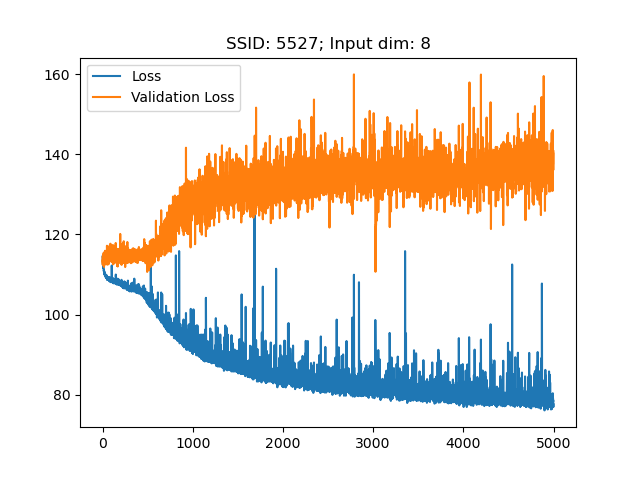
\includegraphics[scale=0.40]{images/NegativeTransferLearning}
    \caption{An instance of negative transfer learning.}
    \label{fig:NegativeTransferLearning}
\end{figure}



\iffalse
\begin{figure}[h]% [H] is so declass\'e!
\centering
\begin{minipage}{0.45\textwidth}
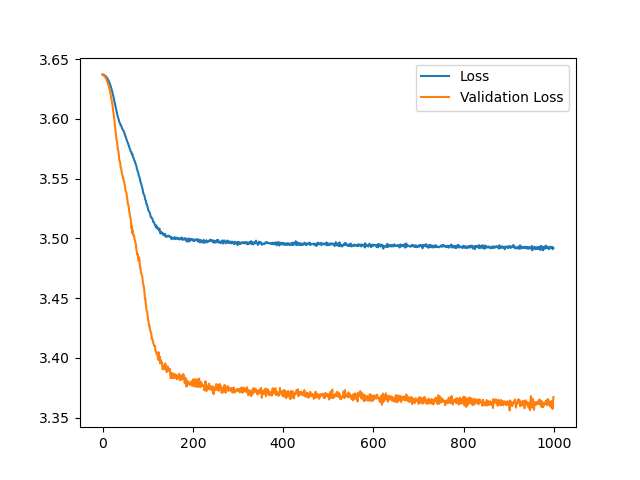
\includegraphics[width=\textwidth]{images/GoodLossCurve4796}
\caption{Good training loss curve (search space ID 4796)}
    \label{fig:GoodLossCurve4796}
\end{minipage}\hfill
\begin{minipage}{0.45\textwidth}
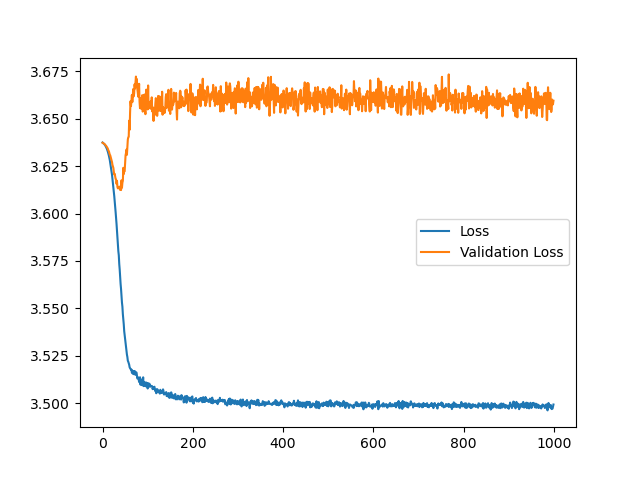
\includegraphics[width=\textwidth]{images/NegativeLearning5860}
\caption{Bad training loss curve (search space ID 5896)}
    \label{fig:NegativeLearning5860}
\end{minipage}
\end{figure}


\begin{figure}[h]
  \centering
    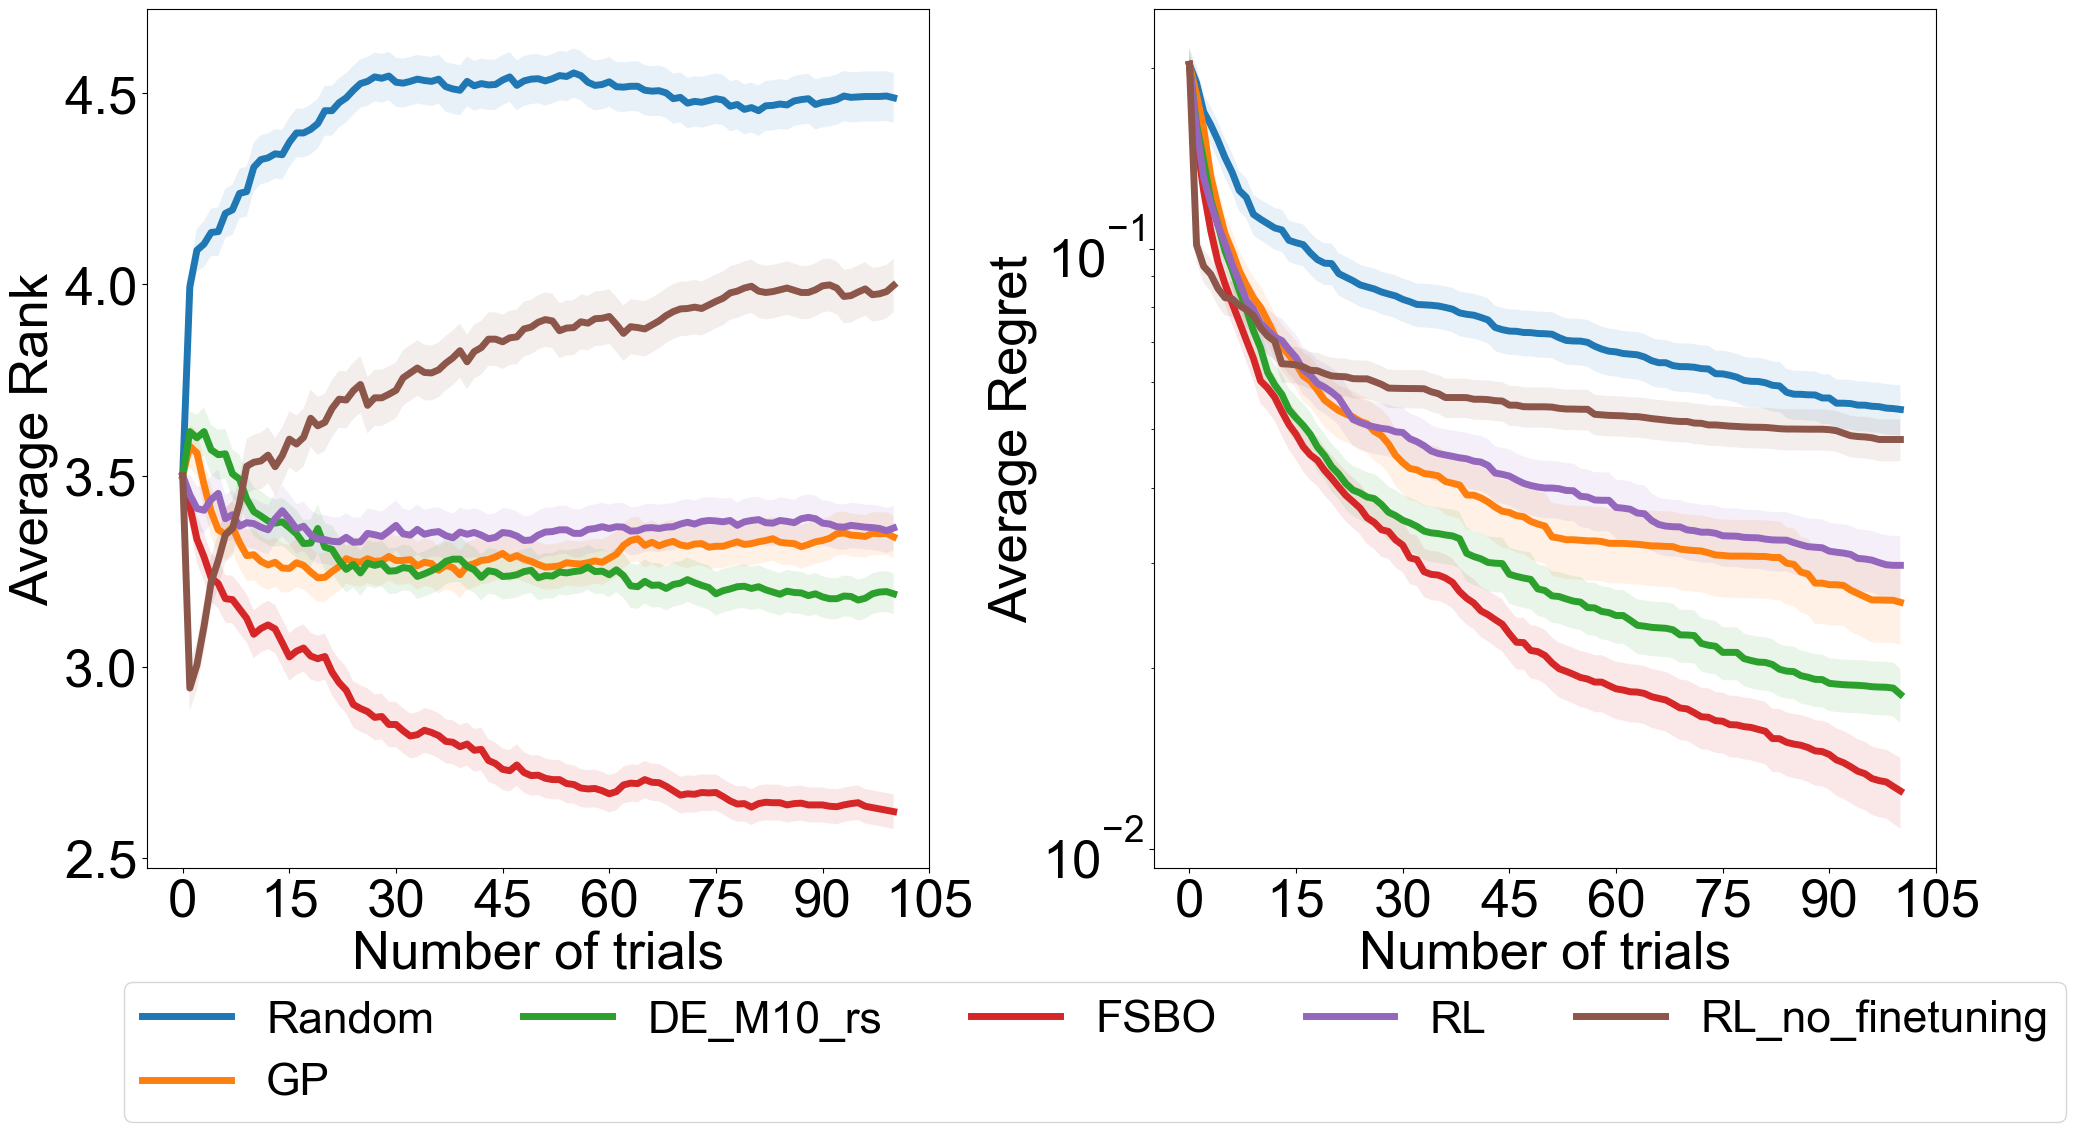
\includegraphics[scale=0.25]{images/RLEvaluationBasicScoring}
    \caption{Benchmarking basic scoring model trained using ListMLE}
    \label{fig:RLEvaluationBasicScoring}
\end{figure}
\fi

\subsection{Study of ranking losses}

In this section, we discuss the following question - are ranking losses better for HPO than regression ones? Secondly, which ranking loss is better for HPO: point-wise,  pair-wise, or list-wise loss?
For the regression case,  we use the Deep Ensemble baseline implementation proposed by Lakshminarayanan et al. ~\cite{DeepEnsemblePaper} as a reference. We use subset regression,  RankNet, and ListMLE loss functions for point-wise, rank-wise, and list-wise ranking losses, respectively. 

\subsubsection{Non transfer HPO}
We first test the non-transfer HPO case where the surrogate models are not meta-trained. We only do fine-tune (or training) during the evaluation phase. We also reinitialize the models before every evaluation step. We have discussed the reason for this in-depth in Section~\ref{sec:rlfinetune}.
We train each neural network for 1000 epochs at every evaluation step. The learning rate is 0.02, and we do not use cosine annealing.
Using cosine annealing here did not make sense since there is no guarantee that the randomly initialized model is near a local optimum.
Hence, we need a bigger learning rate to find quicker optimization.
We try to keep all the parameters the same as the best case of DE results (Our reference method for the non Transfer HPO case)

\begin{figure}[h]
  \centering
    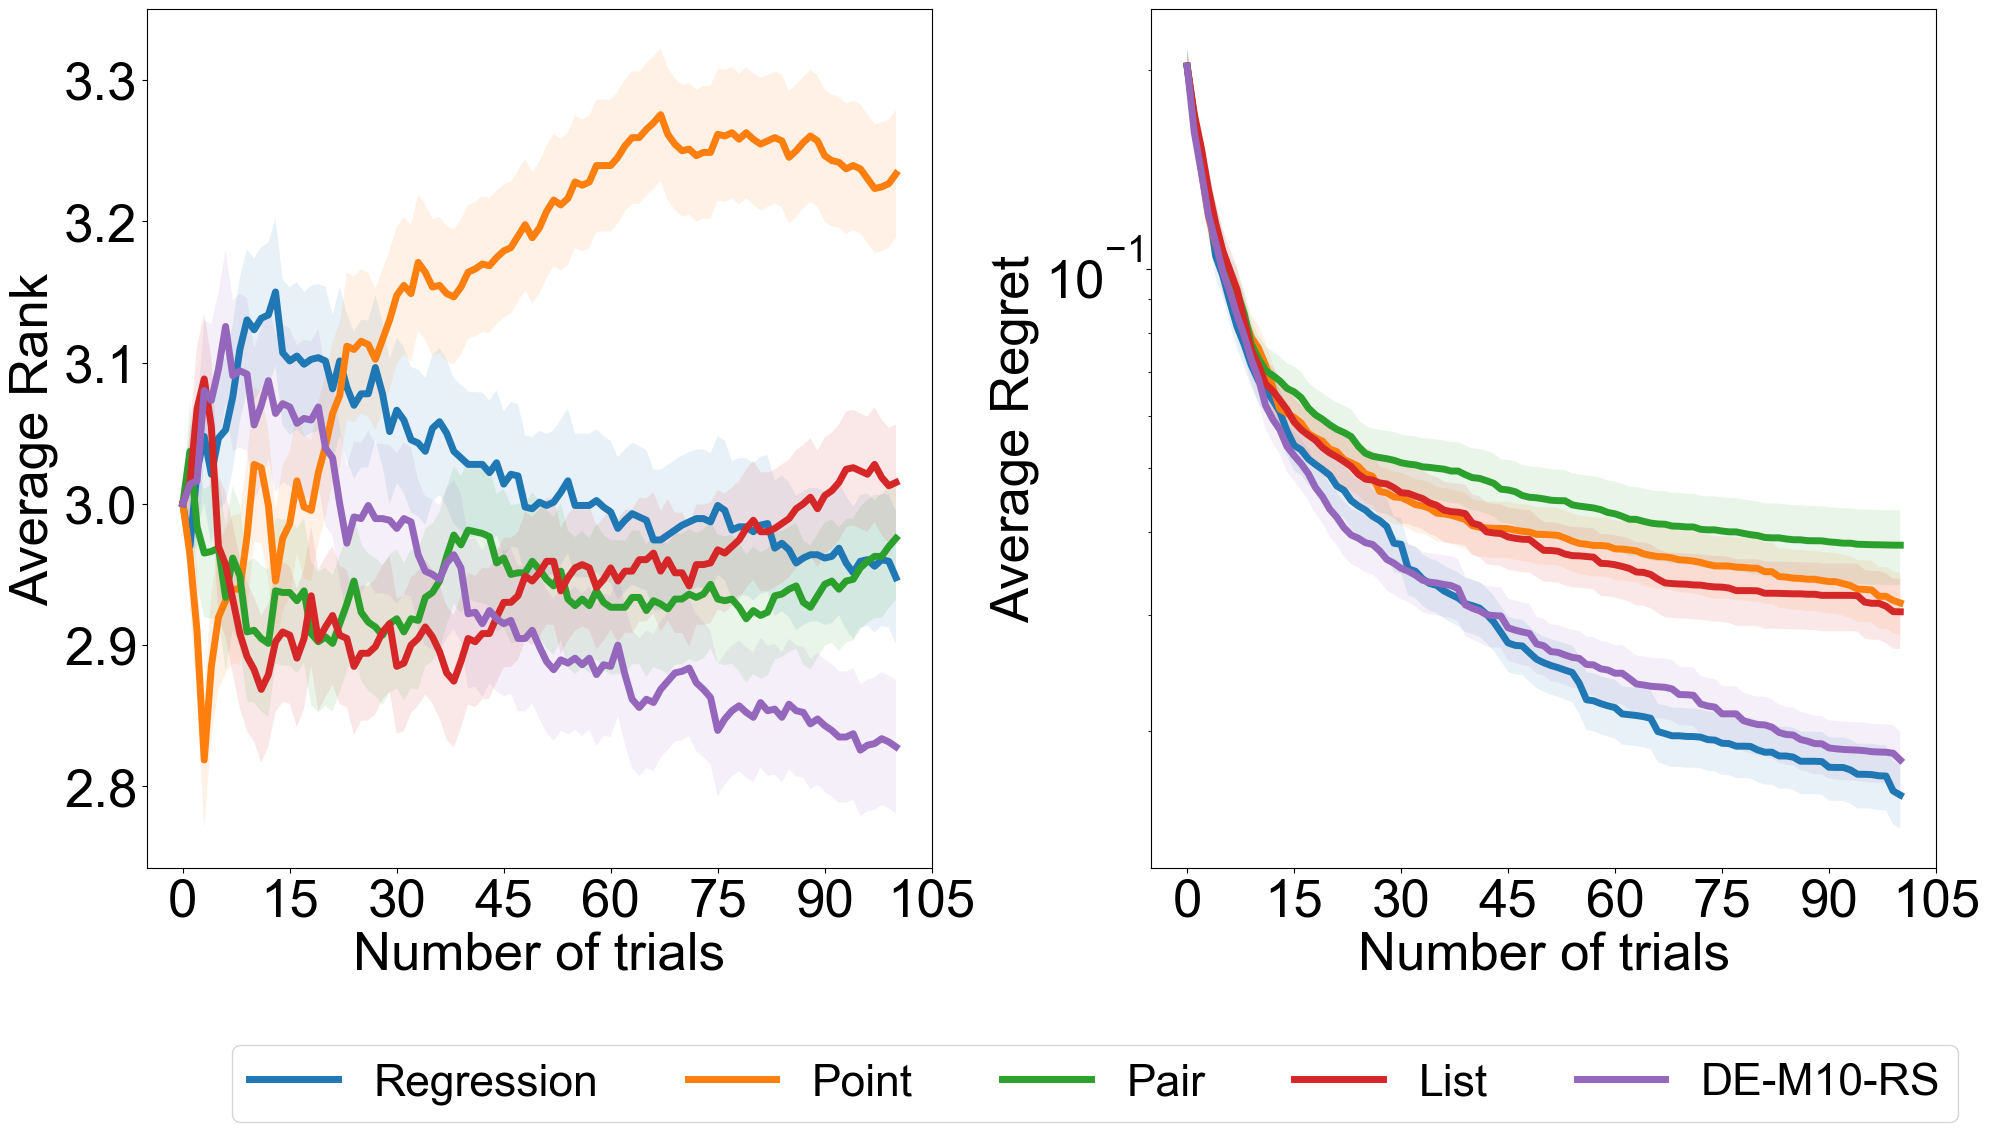
\includegraphics[scale=0.25]{images/Q1AblationNonTransfer}
    \caption{Comparison of Ranking losses with regression losses (Non transfer case)}
    \label{fig:Q1AblationNonTransfer}
\end{figure}

Firstly, we see that the average regret for both the regression losses is similar. This result is expected because the only significant difference between the two models is how uncertainty is modeled. Secondly,  we see from Figure~\ref{fig:Q1AblationNonTransfer} that the models trained with ranking losses are better at the beginning of the optimization steps cycle than the regression losses. This can be seen in the critical rank graphs of Figure~\ref{fig:Q1AblationNonTransferRank100} as well. However, the pointwise loss function very quickly deteriorates in performance in the long run. The pointwise loss function tries to learn the rank directly from the input. The learned ranks also depend on the other HP configurations in a given batch. Hence this loss function does not train the model to learn relative differences in the HP configurations.



\begin{figure}[h]% [H] is so declass\'e!
\centering
\begin{minipage}{0.45\textwidth}
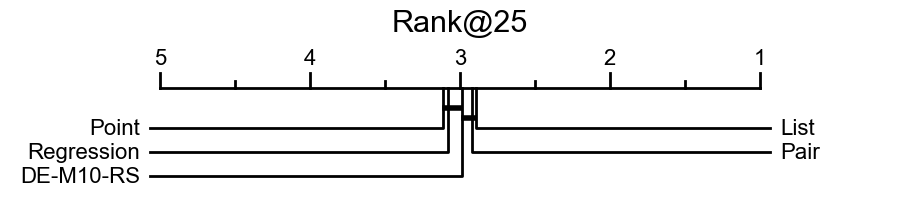
\includegraphics[width=\textwidth]{images/Q1AblationNonTransferRank@25}
\end{minipage}\hfill
\begin{minipage}{0.45\textwidth}
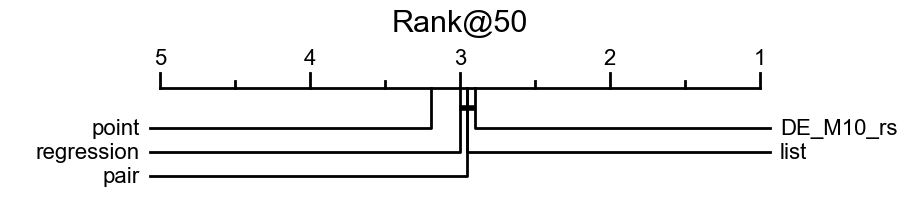
\includegraphics[width=\textwidth]{images/Q1AblationNonTransferRank@50}
\end{minipage}\par
\vskip\floatsep% normal separation between figures
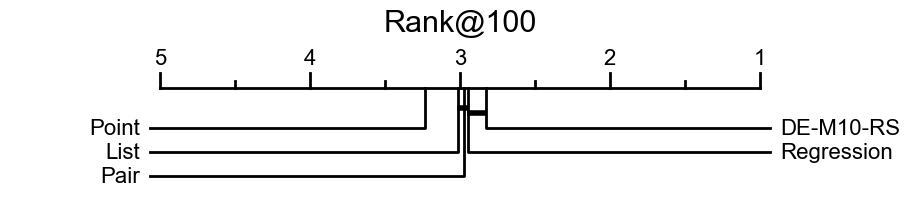
\includegraphics[width=0.45\textwidth]{images/Q1AblationNonTransferRank@100}
    \caption{Critical rank graph of the non transfer ablation study (Non transfer case)}
   \label{fig:Q1AblationNonTransferRank100}
\end{figure}


\subsubsection{Transfer HPO}
In the transfer HPO case,  we first train the models with the meta-training data given by the HPO-B data set and then store our models on persistent storage.
We train the models for 5000 epochs with a fixed learning rate of 0.001.
We used a batch size of 100 for all models. We used a list size of 100 for the list-wise loss functions.
However, we use cosine annealing during fine-tuning for the reasons discussed in Section~\ref{sec:rlfinetune}.
It is because there is a very high chance that the learned model is close to any one of the local optima (the exception to this is the negative learning rate case discussed later).

The selection of batches of HP configuration for training is not trivial.
For any given search space,  we have data on multiple tasks.
As the distribution of HP configurations may differ for different tasks, we need to learn to rank the HP configurations against other configurations within the same task.
Hence, for each step within an epoch (i.e., for the number of batches within the epoch),  we randomly select a task (i.e., meta-dataset) and then select the HP configurations within this task.
This sampling mechanism is the double sampling mechanism we discussed in Section~\ref{sec:rlmetatraining}.
Double sampling is not required during fine-tuning as we are fine-tuning only for a particular task.

\begin{figure}[h]
  \centering
    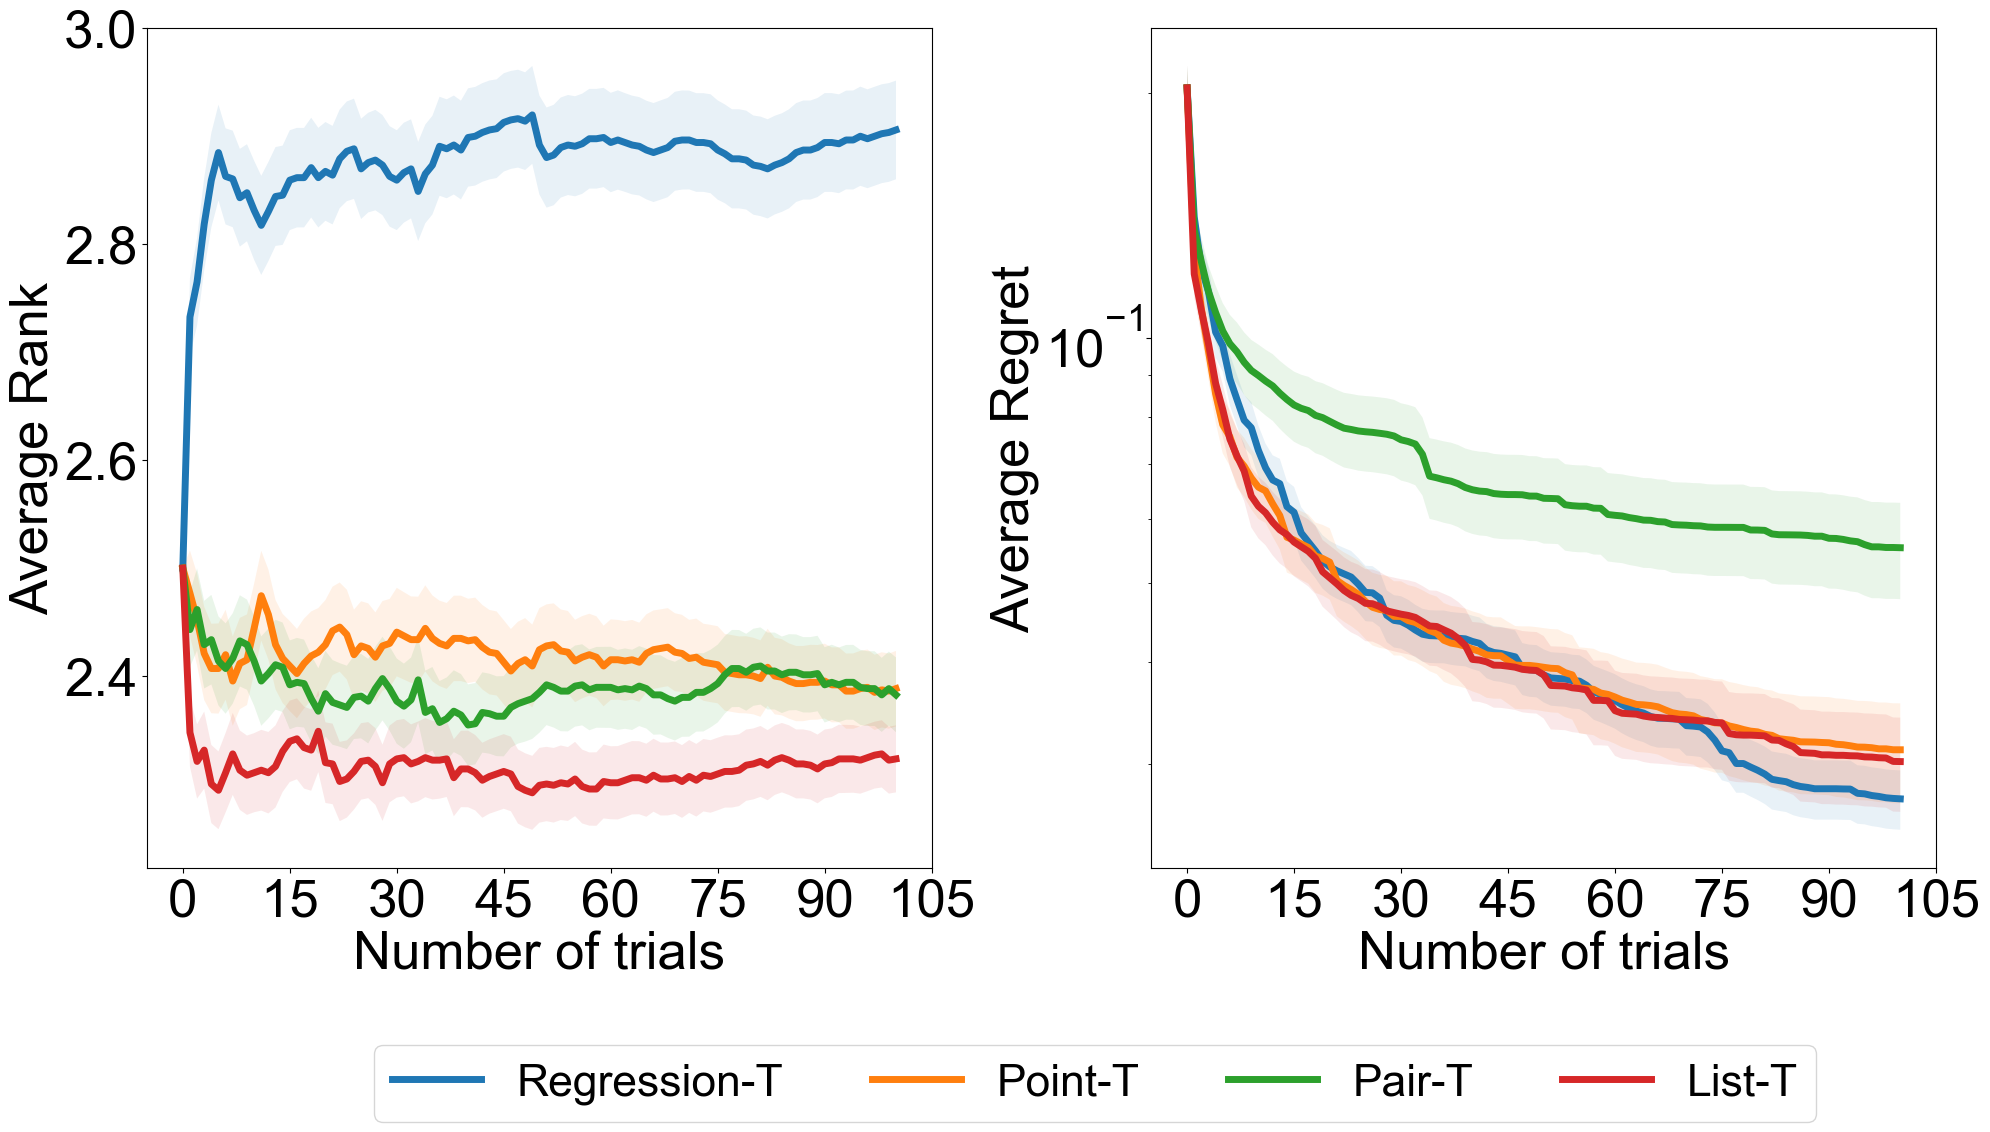
\includegraphics[scale=0.25]{images/Q1AblationTransfer}
    \caption{Comparison of Ranking losses with regression losses (Transfer case)}
    \label{fig:Q1AblationTransfer}
\end{figure}

Figure~\ref{fig:Q1AblationTransfer} compares the average regret and the ranking graph for the regression and ranking losses for the transfer case.
As we can see here,  the listwise ranking losses are far superior to other losses.
It is also interesting to see that the average regret of the list-wise losses is similar to the regression losses in the transfer case.
To check the overall performance of the list-wise loss models, we compare this model with the worst,  medium, and best performing surrogates as sentinels for the study.
The random selection strategy is the worst performing,  whereas FSBO is the best performing SMBO surrogate. We use a GP surrogate to represent a surrogate with a medium performance.
Figure~\ref{fig:Q1FinalAblation} shows this ablation.
The list-wise loss function functions better than the state-of-the-art transfer HPO model "FSBO" in the first 15 to 20 evaluation steps.

\begin{figure}[h]
  \centering
    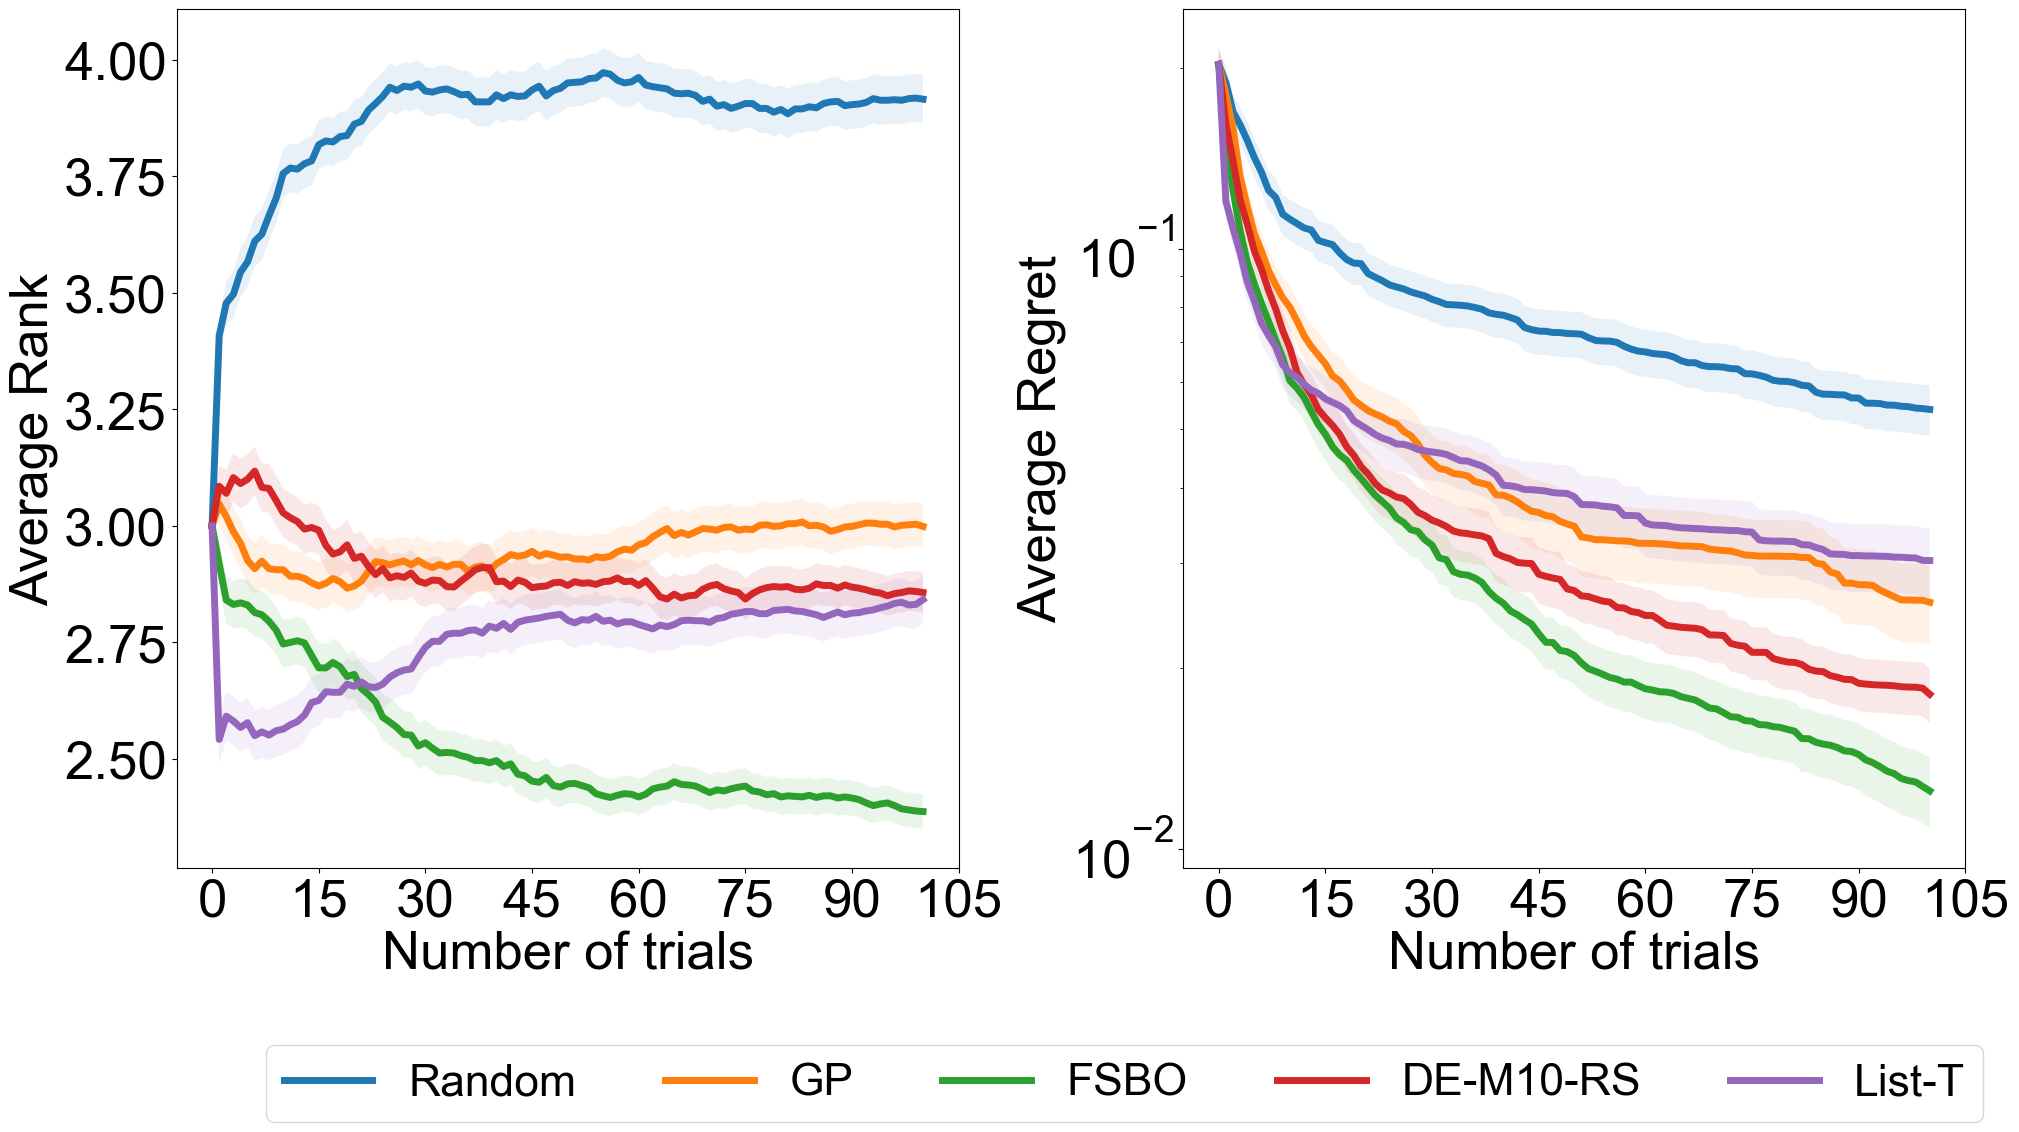
\includegraphics[scale=0.25]{images/Q1FinalAblation}
    \caption{Comparison of list-wise transfer with standard HPO surrogates}
    \label{fig:Q1FinalAblation}
\end{figure}


\subsection{Study of weighted list Wise losses}

In Section~\ref{sec:positionEnhancedRanking} we discussed the requirement for weighting for our problem.
This section presents a short ablation to study its effect on our models.
We do not separate the transfer and non-transfer cases here.
We use inverse log weighting for the weighting in our case.
From Figure~\ref{fig:Q2Ablation}, we see that both in the case of transfer HPO and non-transfer HPO, the weighting positively impacted the performance. Moreover, the models trained with weighted list-wise losses are better at every optimization cycle step.

Even though the difference in the average regret is not significant in the 4 cases,  the ranking graph differences are pretty significant. One thing to note here is that when we use list-wise loss,  we train and fine-tune with the same weighted loss. We do not use a different weighting (like the inverse linear weighting for training and inverse log weighting for the meta training). Moreover, we use the double sampling mechanism discussed above during meta-training.

\begin{figure}[h]
  \centering
    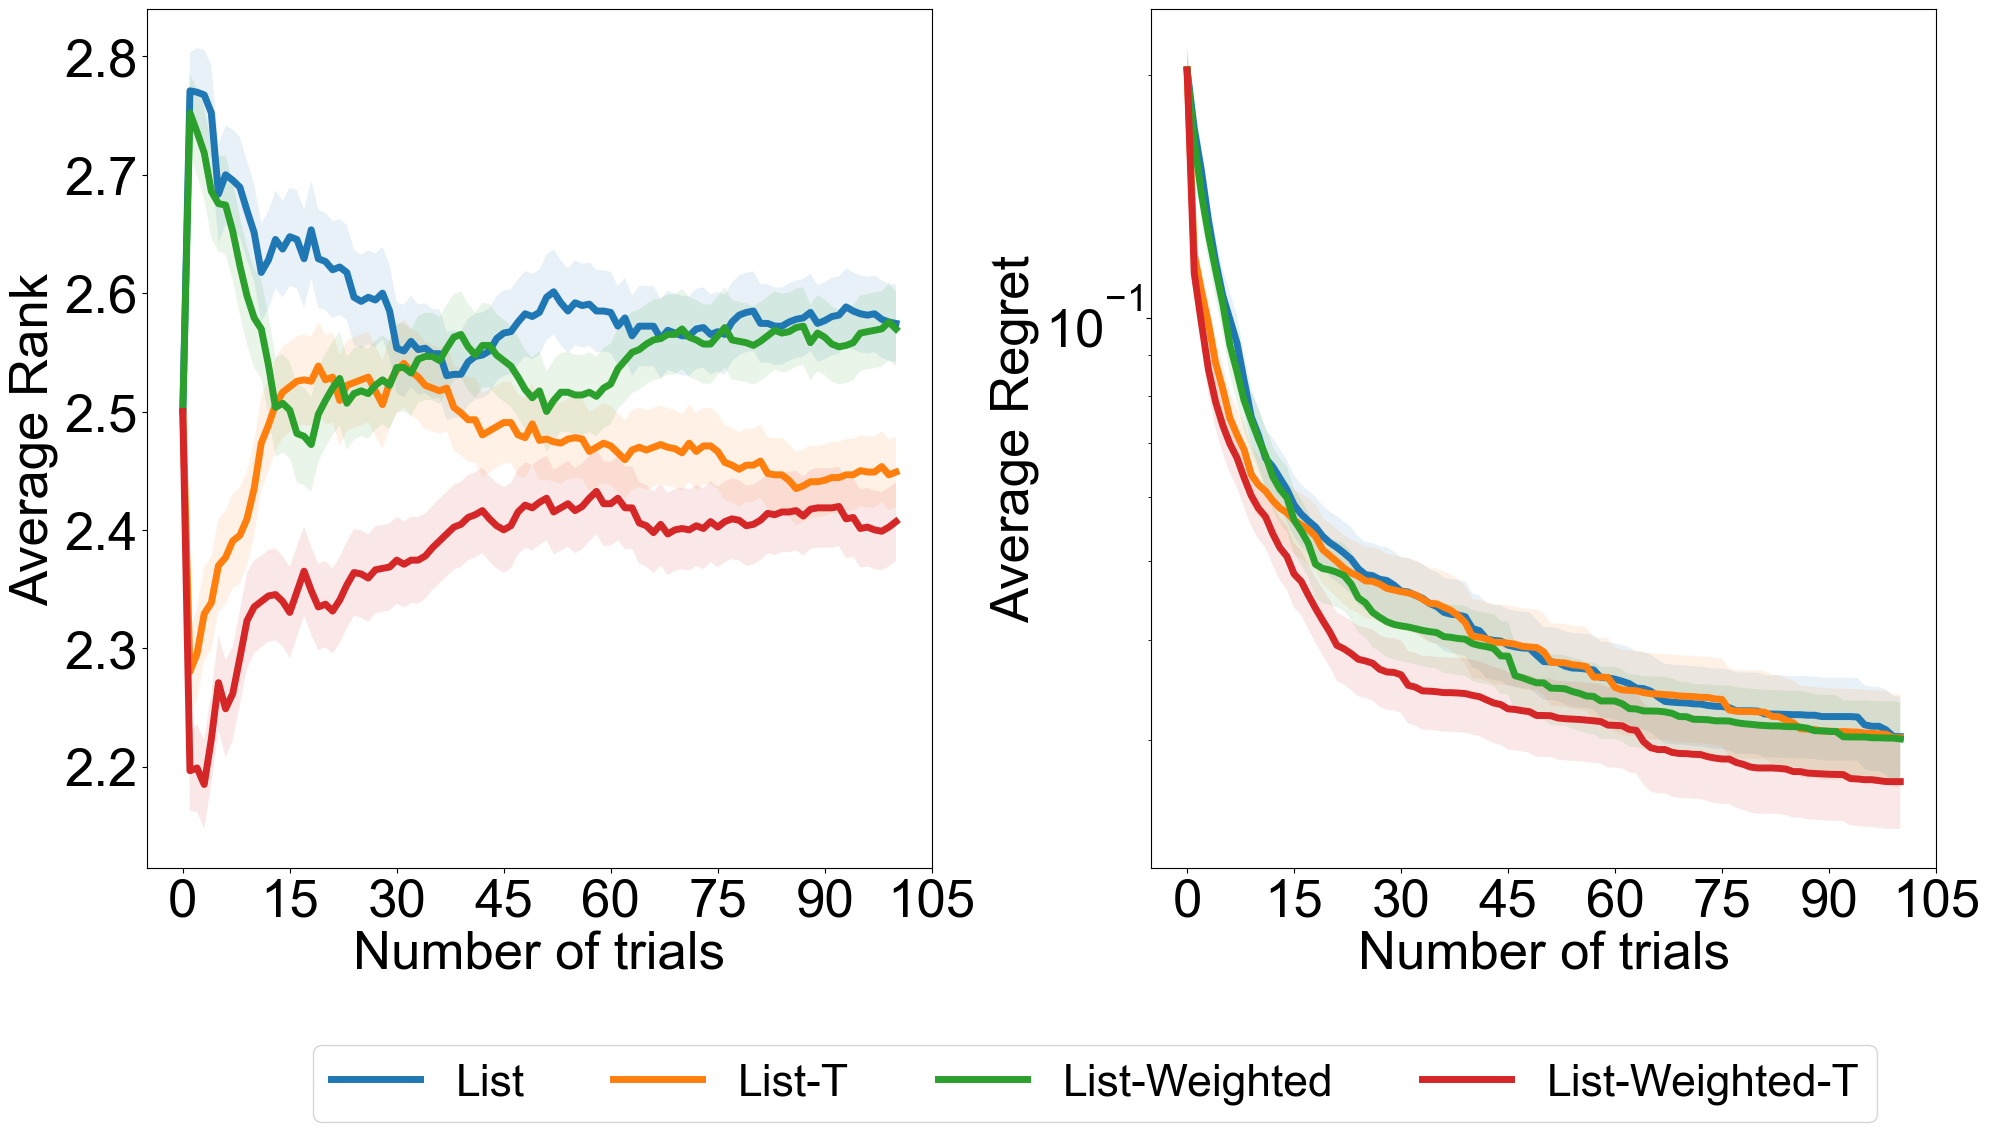
\includegraphics[scale=0.25]{images/Q2Ablation}
    \caption{Comparison of list-wise transfer with standard HPO surrogates}
    \label{fig:Q2Ablation}
\end{figure}


\subsection{Study of Surrogate Design: Addition of Deep Sets}

We found in our research that our model could be improved by making it context-aware. We used an architecture with deep sets described in Section~\ref{sec:DeepSetWithModel}. As previously discussed, the latent result of the deep-set is used as a context for the scoring model. To meta-train this architecture,  we needed to change the training and sampling mechanisms.

For sampling, we used a support set of data points, i.e., \{$X_s$, $y_s$\} that is 20\% of the actual batch size. The concept of double sampling is also used in this case. For each double sampling, we sample first the task.
Then the support points are sampled without replacement from this task.
Subsequently, we sample the query points $X_q$ based on the batch size and list size (By default, 100 for both).
During meta tuning, we must also have a support and query set for training.
We again use 20\% of the points as support points and the rest as query points during the fine-tuning process.

One major issue when training with deep sets is that we cannot train the neural networks separately.
It is because of the common backbone in ensemble architecture.
In order to keep the training as separate as possible, we initialize the neural networks separately. After that, we calculate the loss of each neural network separately with the same batch data. Then we aggregate the losses and back-propagate the aggregated loss through the whole architecture. Note that we do not aggregate the scores of the neural networks but the ranking losses obtained from each scoring neural network.

Figure~\ref{fig:Q3Ablation} shows the results of this study. In the non-transfer case,  the model becomes terrible. The primary reason for this is that the complexity of the architecture is very high, and it needs a considerable amount of data to train. This data is absent during the HPO optimization cycle. However,  in the case of transfer learning,  we see an enormous improvement when we use deep sets. It makes intuitive sense because each task is different from the other. The embedding of this information, or rather the difference in information, helps the model distinguish the tasks and pre-condition the learning process. 

\begin{figure}[h]
  \centering
    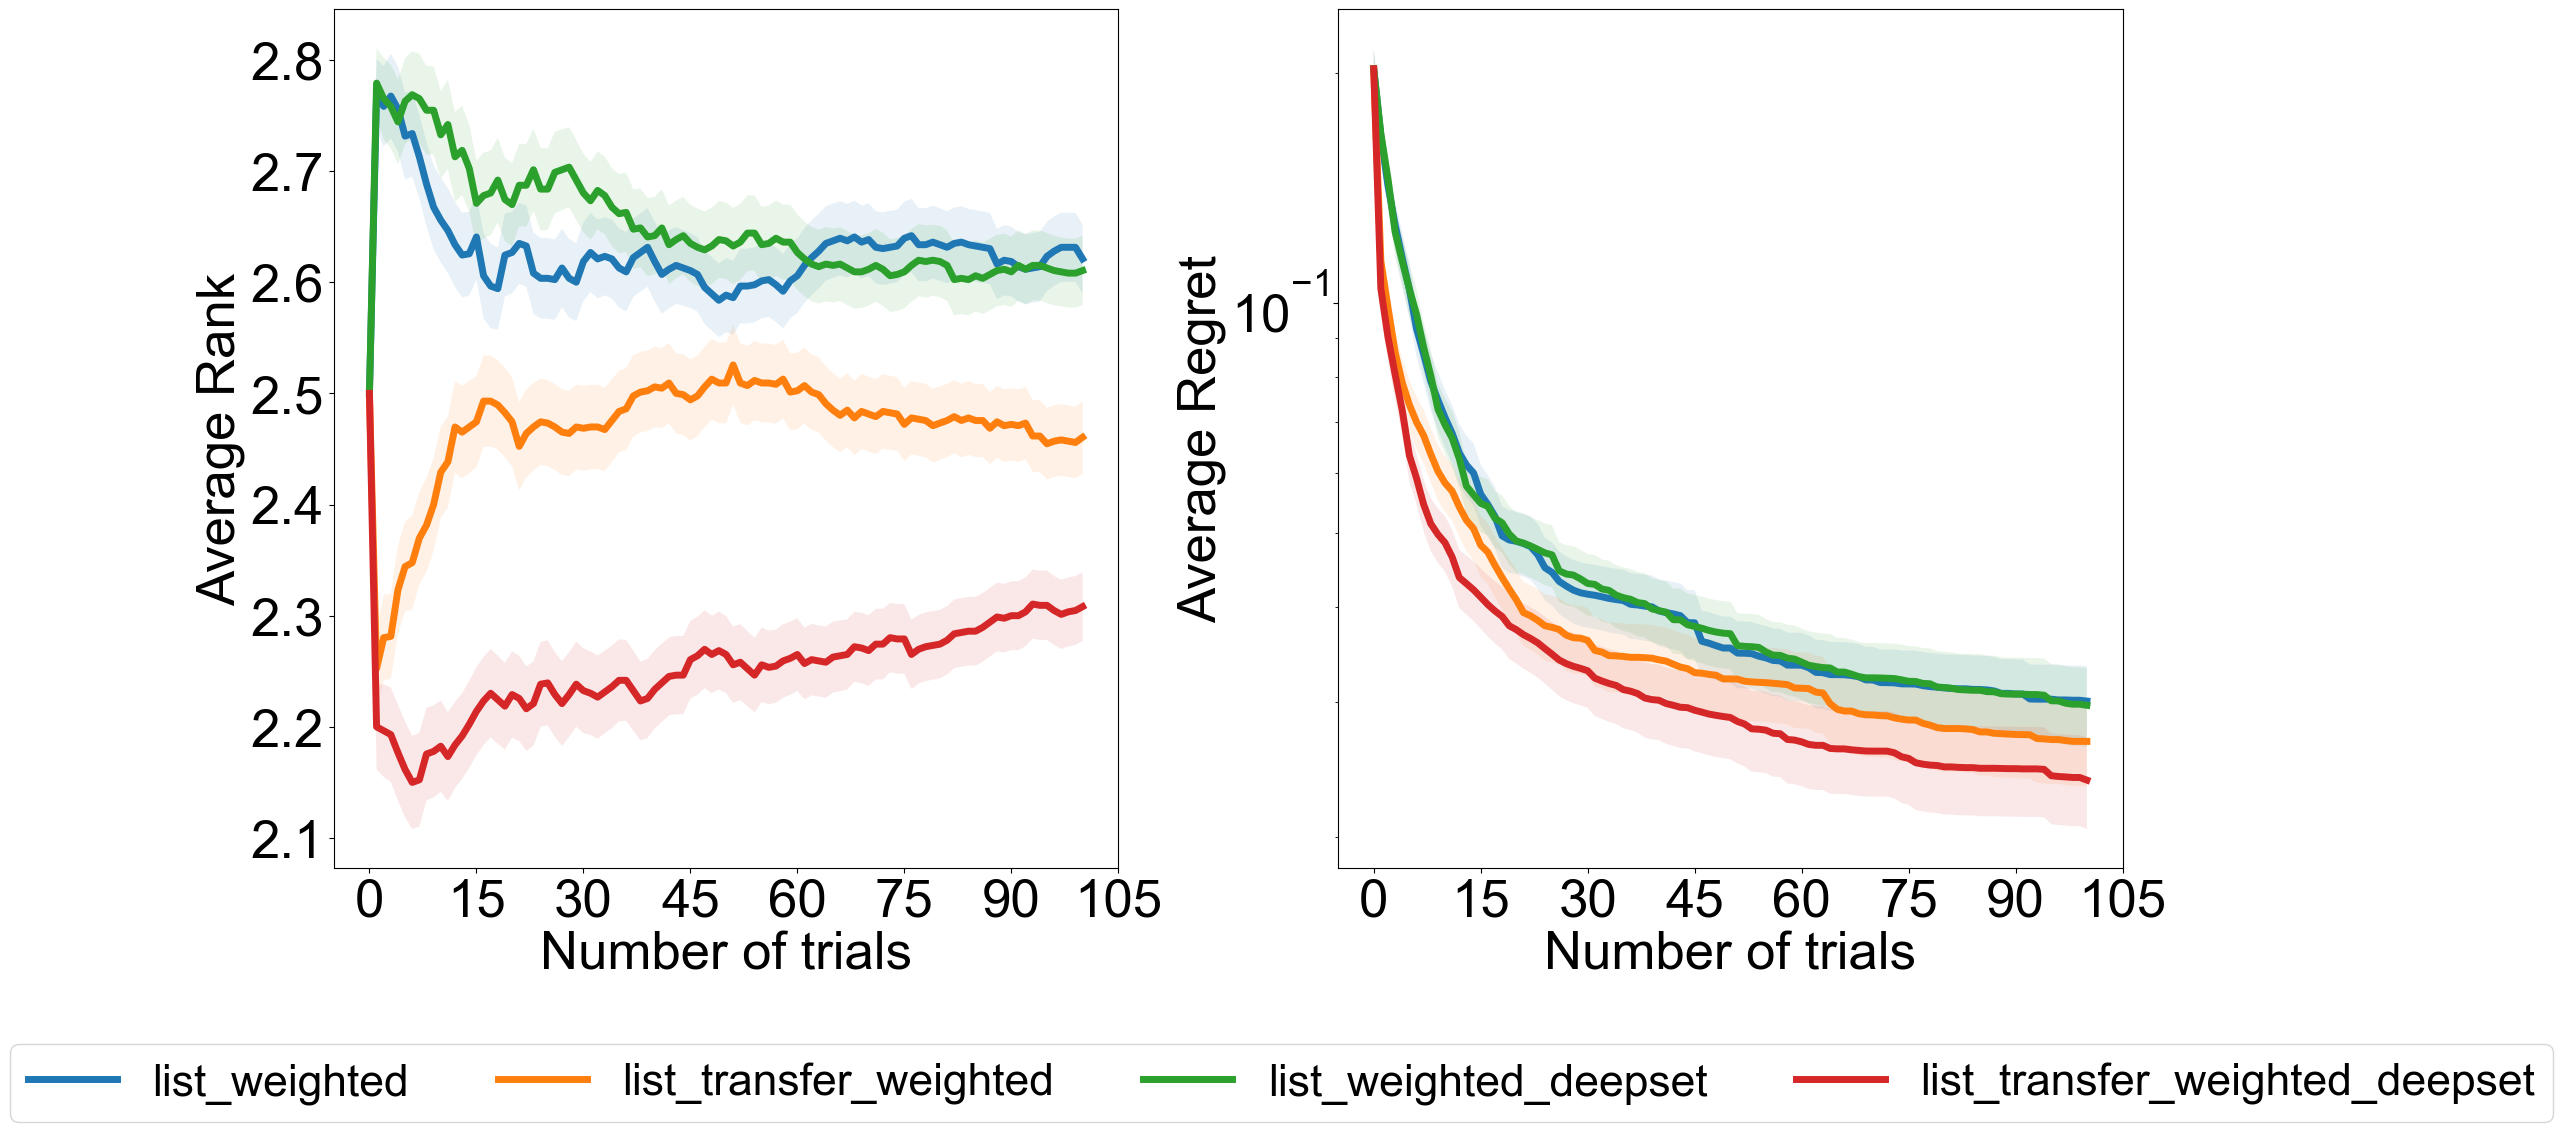
\includegraphics[scale=0.25]{images/Q3Ablation}
    \caption{Studying how the addition of context (Deep Sets) affects our model}
    \label{fig:Q3Ablation}
\end{figure}

We compare the best results obtained so far with the sentinel performances of GP,  FSBO,  and Random search. Figure~\ref{fig:Q3AblationFinal} illustrates this.  Two interesting observations can be made from our results. First,  our model performs significantly well in the first evaluation steps, and the performance later deteriorates w.r.t to state-of-the-art results. Hence,  this model can be used in any transfer HPO case with limited evaluation steps due to the computation budget. Secondly,   the average regret is also significantly better in the initial phase. Hence, we can unequivocally state that our proposed model is a good candidate to consider in any transfer HPO problem. 

\begin{figure}[h]
  \centering
    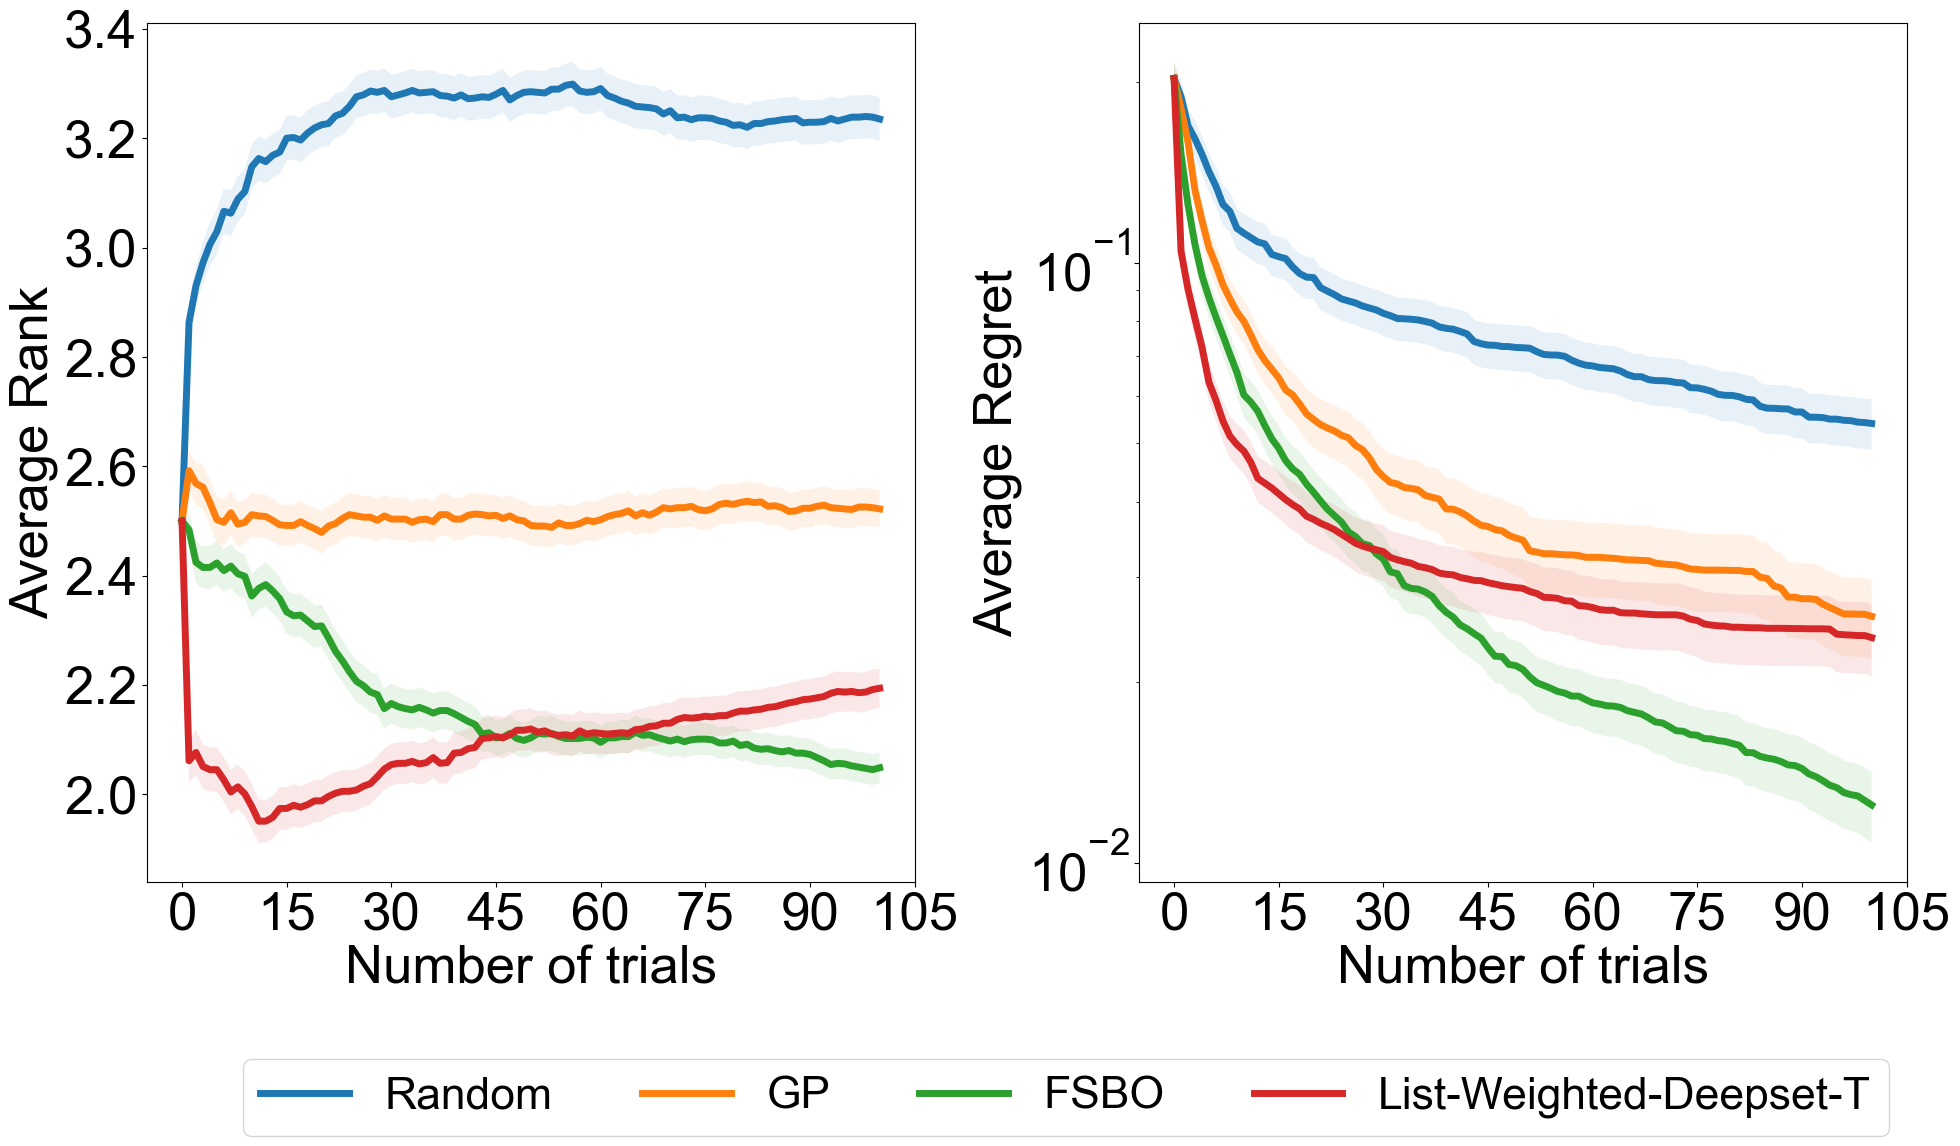
\includegraphics[scale=0.25]{images/Q3AblationFinal}
    \caption{Best model with sentinal HPO performance}
    \label{fig:Q3AblationFinal}
\end{figure}

We also present in Figure~\ref{fig:Q3AblationFinalRank100} the critical rank graphs for reference.

\begin{figure}[h]% [H] is so declass\'e!
\centering
\begin{minipage}{0.45\textwidth}
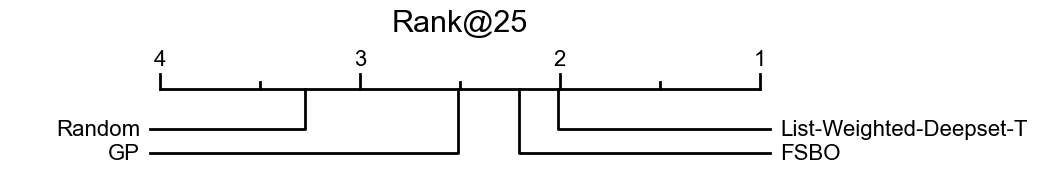
\includegraphics[width=\textwidth]{images/Q3AblationFinalRank@25}
\end{minipage}\hfill
\begin{minipage}{0.45\textwidth}
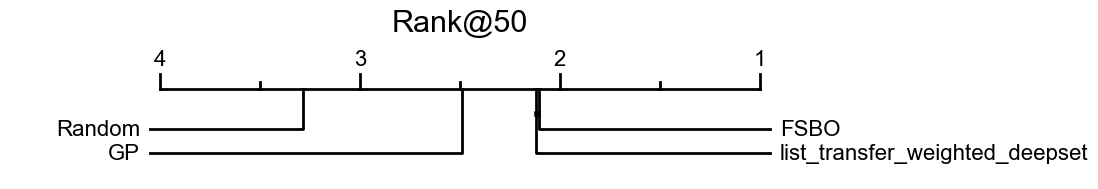
\includegraphics[width=\textwidth]{images/Q3AblationFinalRank@50}
\end{minipage}\par
\vskip\floatsep% normal separation between figures
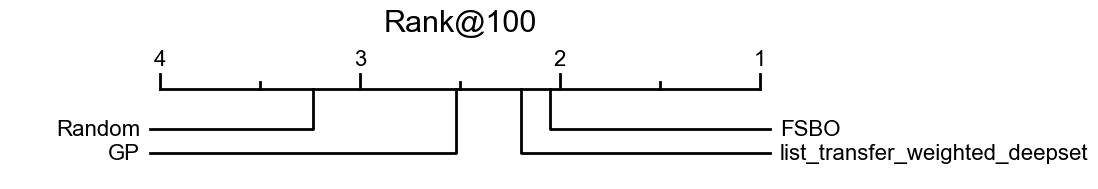
\includegraphics[width=0.45\textwidth]{images/Q3AblationFinalRank@100}
    \caption{Critical rank graph of the list wise weighted transfer learning with deep sets with sentinel performances}
   \label{fig:Q3AblationFinalRank100}
\end{figure}


\iffalse

This is because less relearning happens in fine-tuning due to the addition of context to our model.

During the training however,  we found that the loss curves were very jumpy.

\begin{figure}[h]% [H] is so declass\'e!
\centering
\begin{minipage}{0.45\textwidth}
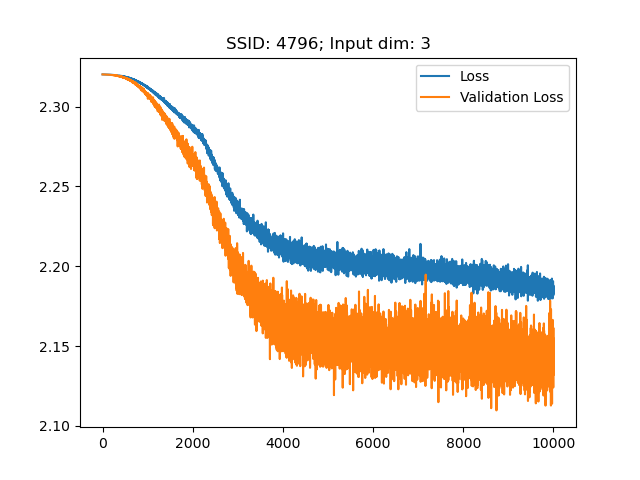
\includegraphics[width=\textwidth]{images/DeepSetLoss4796}
\caption{Loss curve for model with deep set (SSID: 4796)}
    \label{fig:DeepSetLoss4796}
\end{minipage}\hfill
\begin{minipage}{0.45\textwidth}
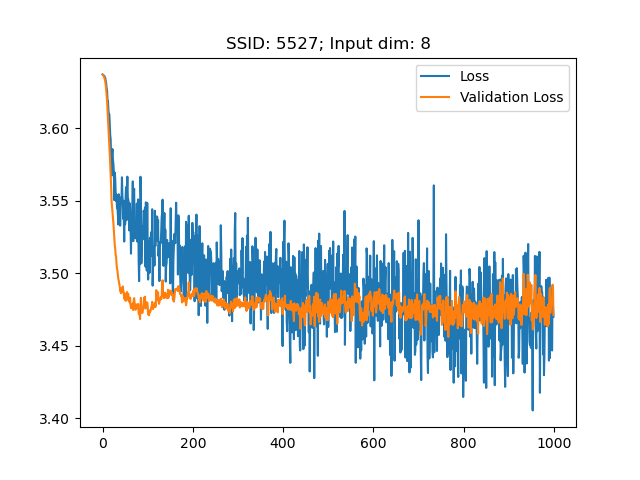
\includegraphics[width=\textwidth]{images/DeepSetLoss5527}
\caption{Loss curve for model with deep set (SSID: 5527)}
    \label{fig:DeepSetLoss5527}
\end{minipage}
\end{figure}

Figure~\ref{fig:DeepSetLoss4796} and Figure~\ref{fig:DeepSetLoss5527} shows this clearly.
We think that this is because of very high representation capacity which is a consequence of using the deep set architecture.

The results of this training and fine tuning our model with deep sets are shown in Figure~\ref{fig:RLDeepSetevaluation}.
In the figure "raw" means that there was no fine tuning performed and the trained model was used as is in the the evaluation/optimization cycle.
One advantage we see with this model is that whether fine tuning is done or not,  the first few evaluations are better than the state of the art results.
This can be seen in the Rank@5 graph critical graph given in Figure~\ref{fig:DeepSetRank5}.
In the later evaluation steps, naturally,  using fine tuning makes gives better performance.

\begin{figure}[h]
  \centering
    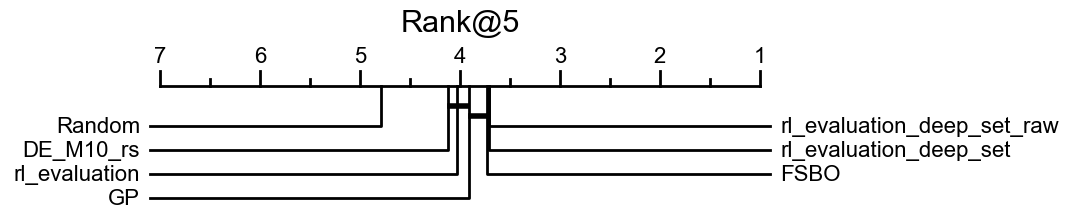
\includegraphics[scale=0.35]{images/DeepSetRank5}
    \caption{Critical rank graph for Model with Deep Set.}
    \label{fig:DeepSetRank5}
\end{figure}

\begin{figure}[h]
  \centering
    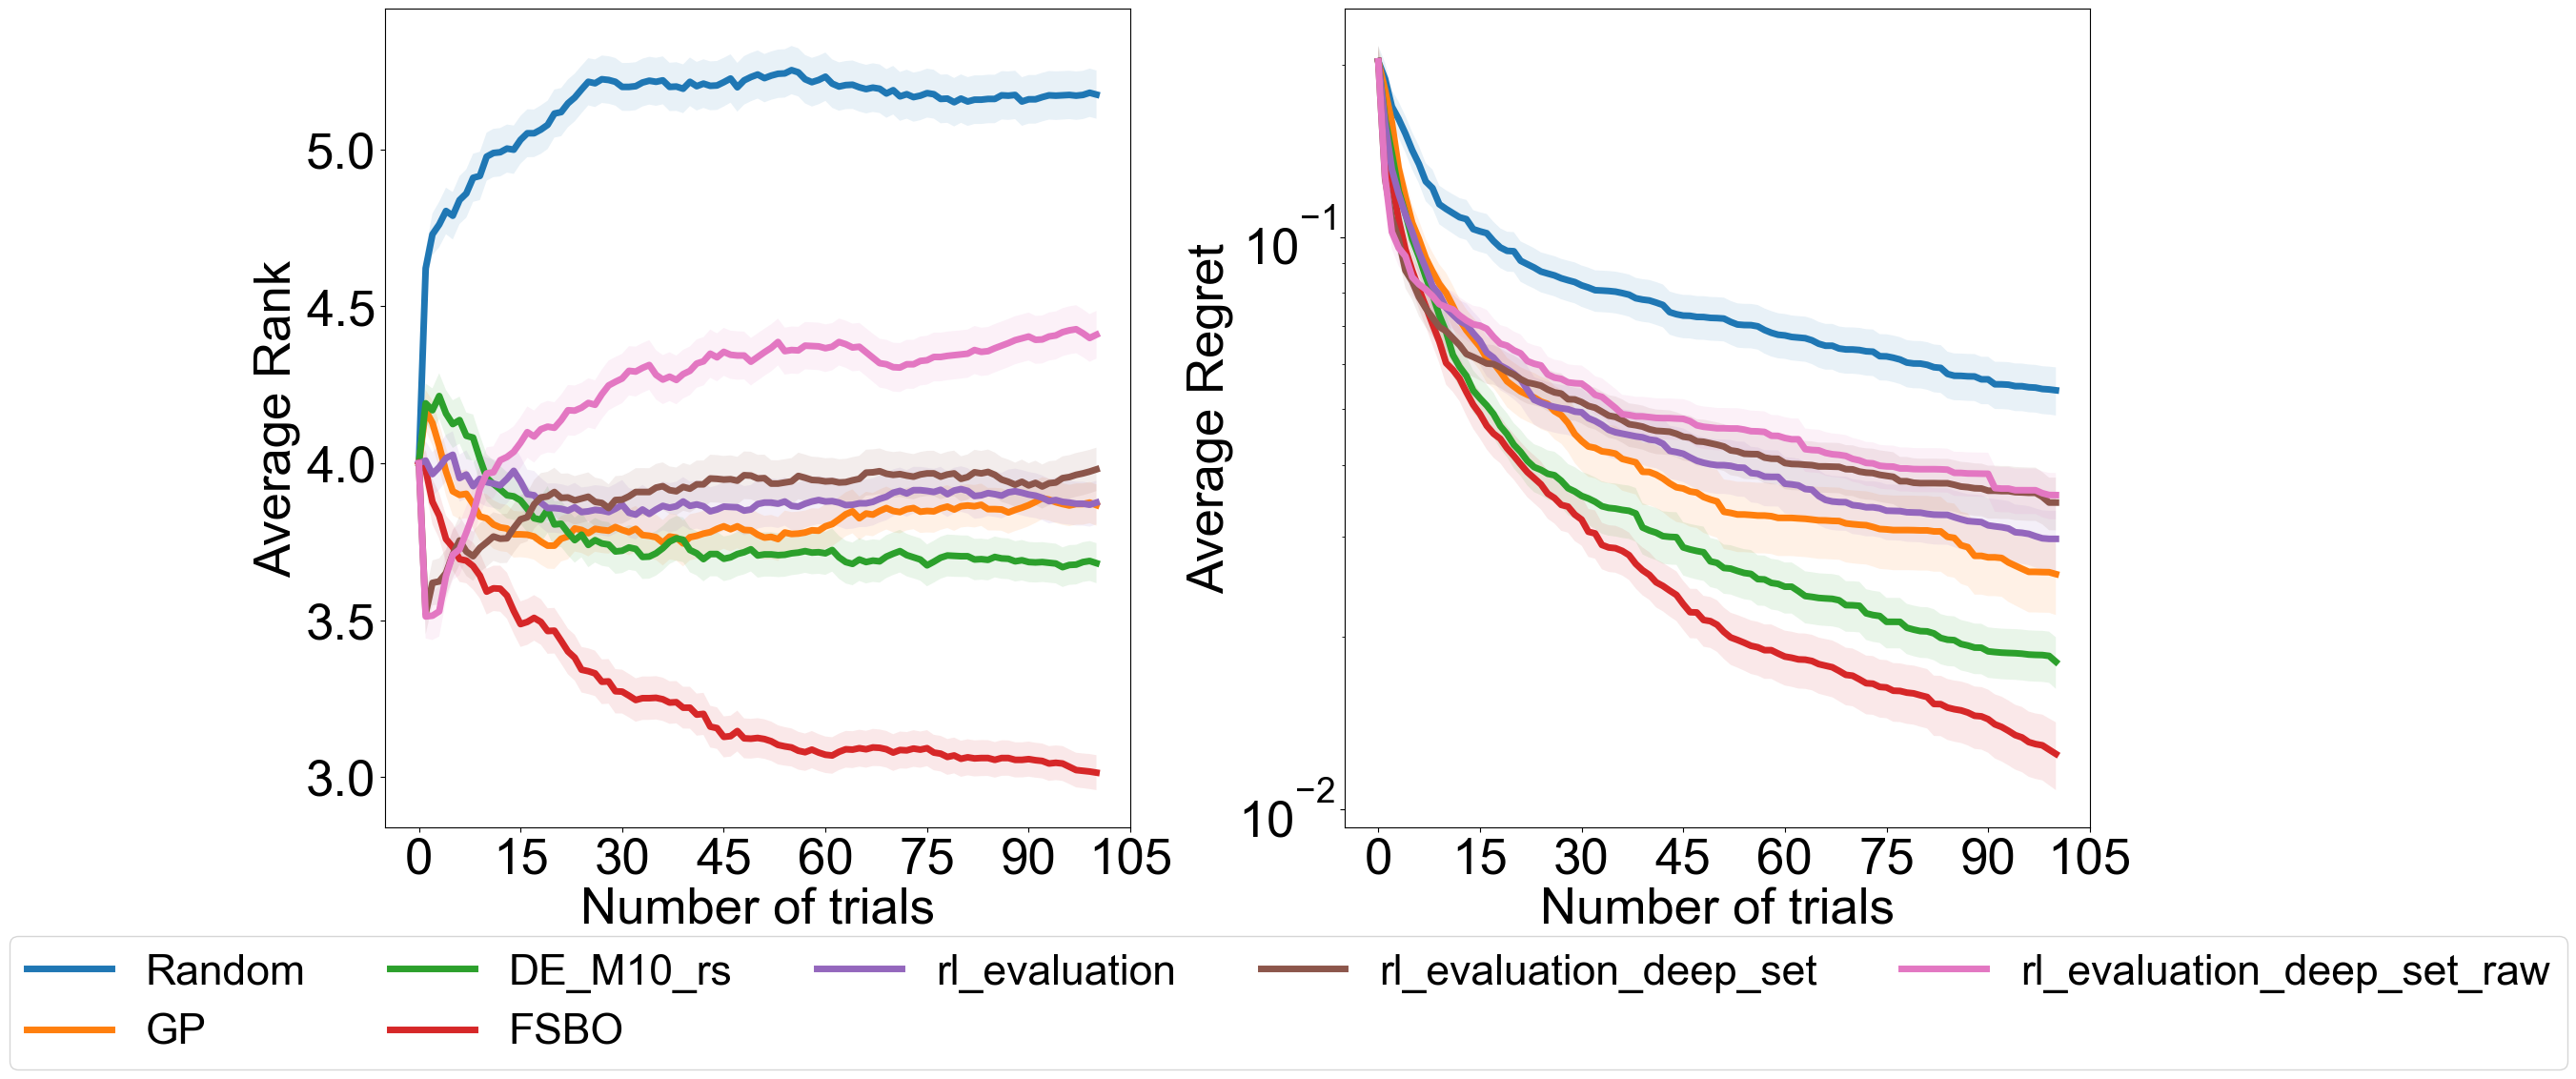
\includegraphics[scale=0.20]{images/RLDeepSetevaluation}
    \caption{Benchmarking for the Deep set evaluation data}
    \label{fig:RLDeepSetevaluation}
\end{figure}
\fi

\iffalse
The fine tuned results is better than all the baselines except FSBO.
In fact,  it is better than FSBO in the first few evaluation steps.
This can be seen in Figure~\ref{fig:RLDeepSetWeightedRank25}.

\begin{figure}[h]
  \centering
    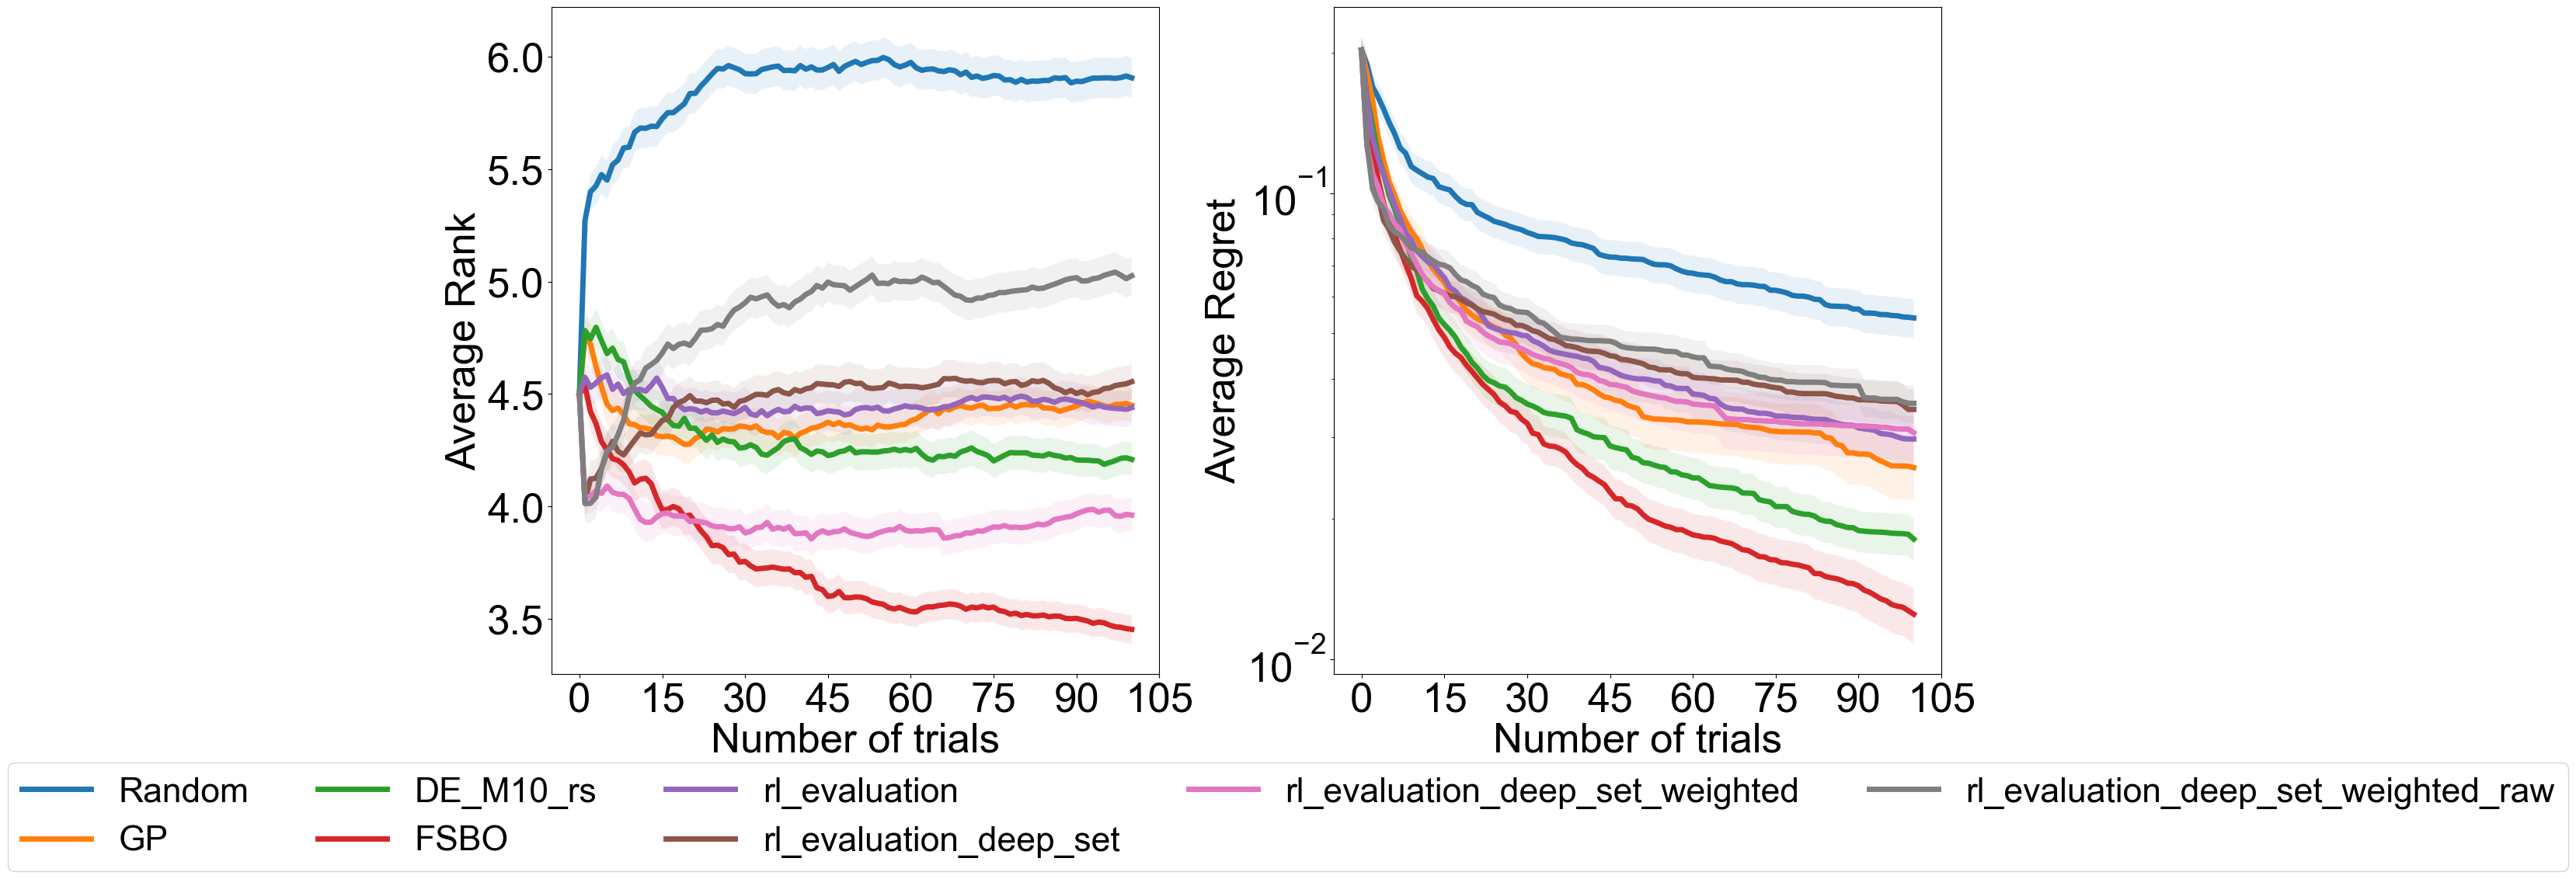
\includegraphics[scale=0.20]{images/RLDeepSetWeighted}
    \caption{Ablation for weighted loss}
    \label{fig:RLDeepSetWeighted}
\end{figure}

\begin{figure}[h]
  \centering
    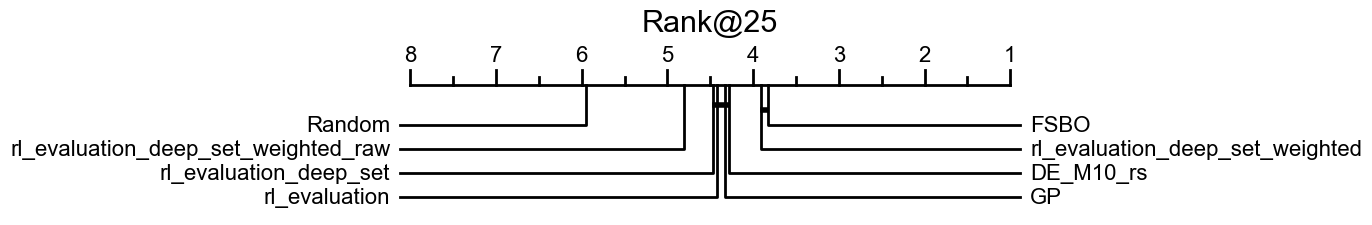
\includegraphics[scale=0.35]{images/RLDeepSetWeightedRank25}
    \caption{Critical rank graph for weighting ablation.}
    \label{fig:RLDeepSetWeightedRank25}
\end{figure}

In this section, we evaluate our built model chronologically, first using the basic scorer model,  then making the model context-aware, and then adding uncertainty capability to the model.
\fi

\subsection{Study of the effect of Fine Tuning}
\label{sec:EffectOfFineTuningResults}
There are two ways of using the meta-trained ranking loss surrogate model. One way is to use it directly without changing it in the optimization process. The other is to finetune it at every evaluation step of the optimization process. We have always used the latter in our ablation studies (or answers to research questions) until now.
In this section, we will see how the performance changes when no finetuning is done during the optimization process.
We take the best model so far to study how finetuning affects performance. Then we run the optimization process with and without finetuning and plot the ranking and regret graphs.

If we do not use any finetuning, selecting the HP configurations for the evaluation process boils down to ranking the set of all unknown HP configurations. Then we select the ranked HP configurations one by one from this ranked list. Finetuning can be understood as a more sophisticated form of the optimization process in which the ranking loss surrogate tries to learn/understand the context from the known HP configurations. Figure~\ref{fig:FineTuningAblation} shows the graphs of models with and without finetuning.

\begin{figure}[h]
  \centering
    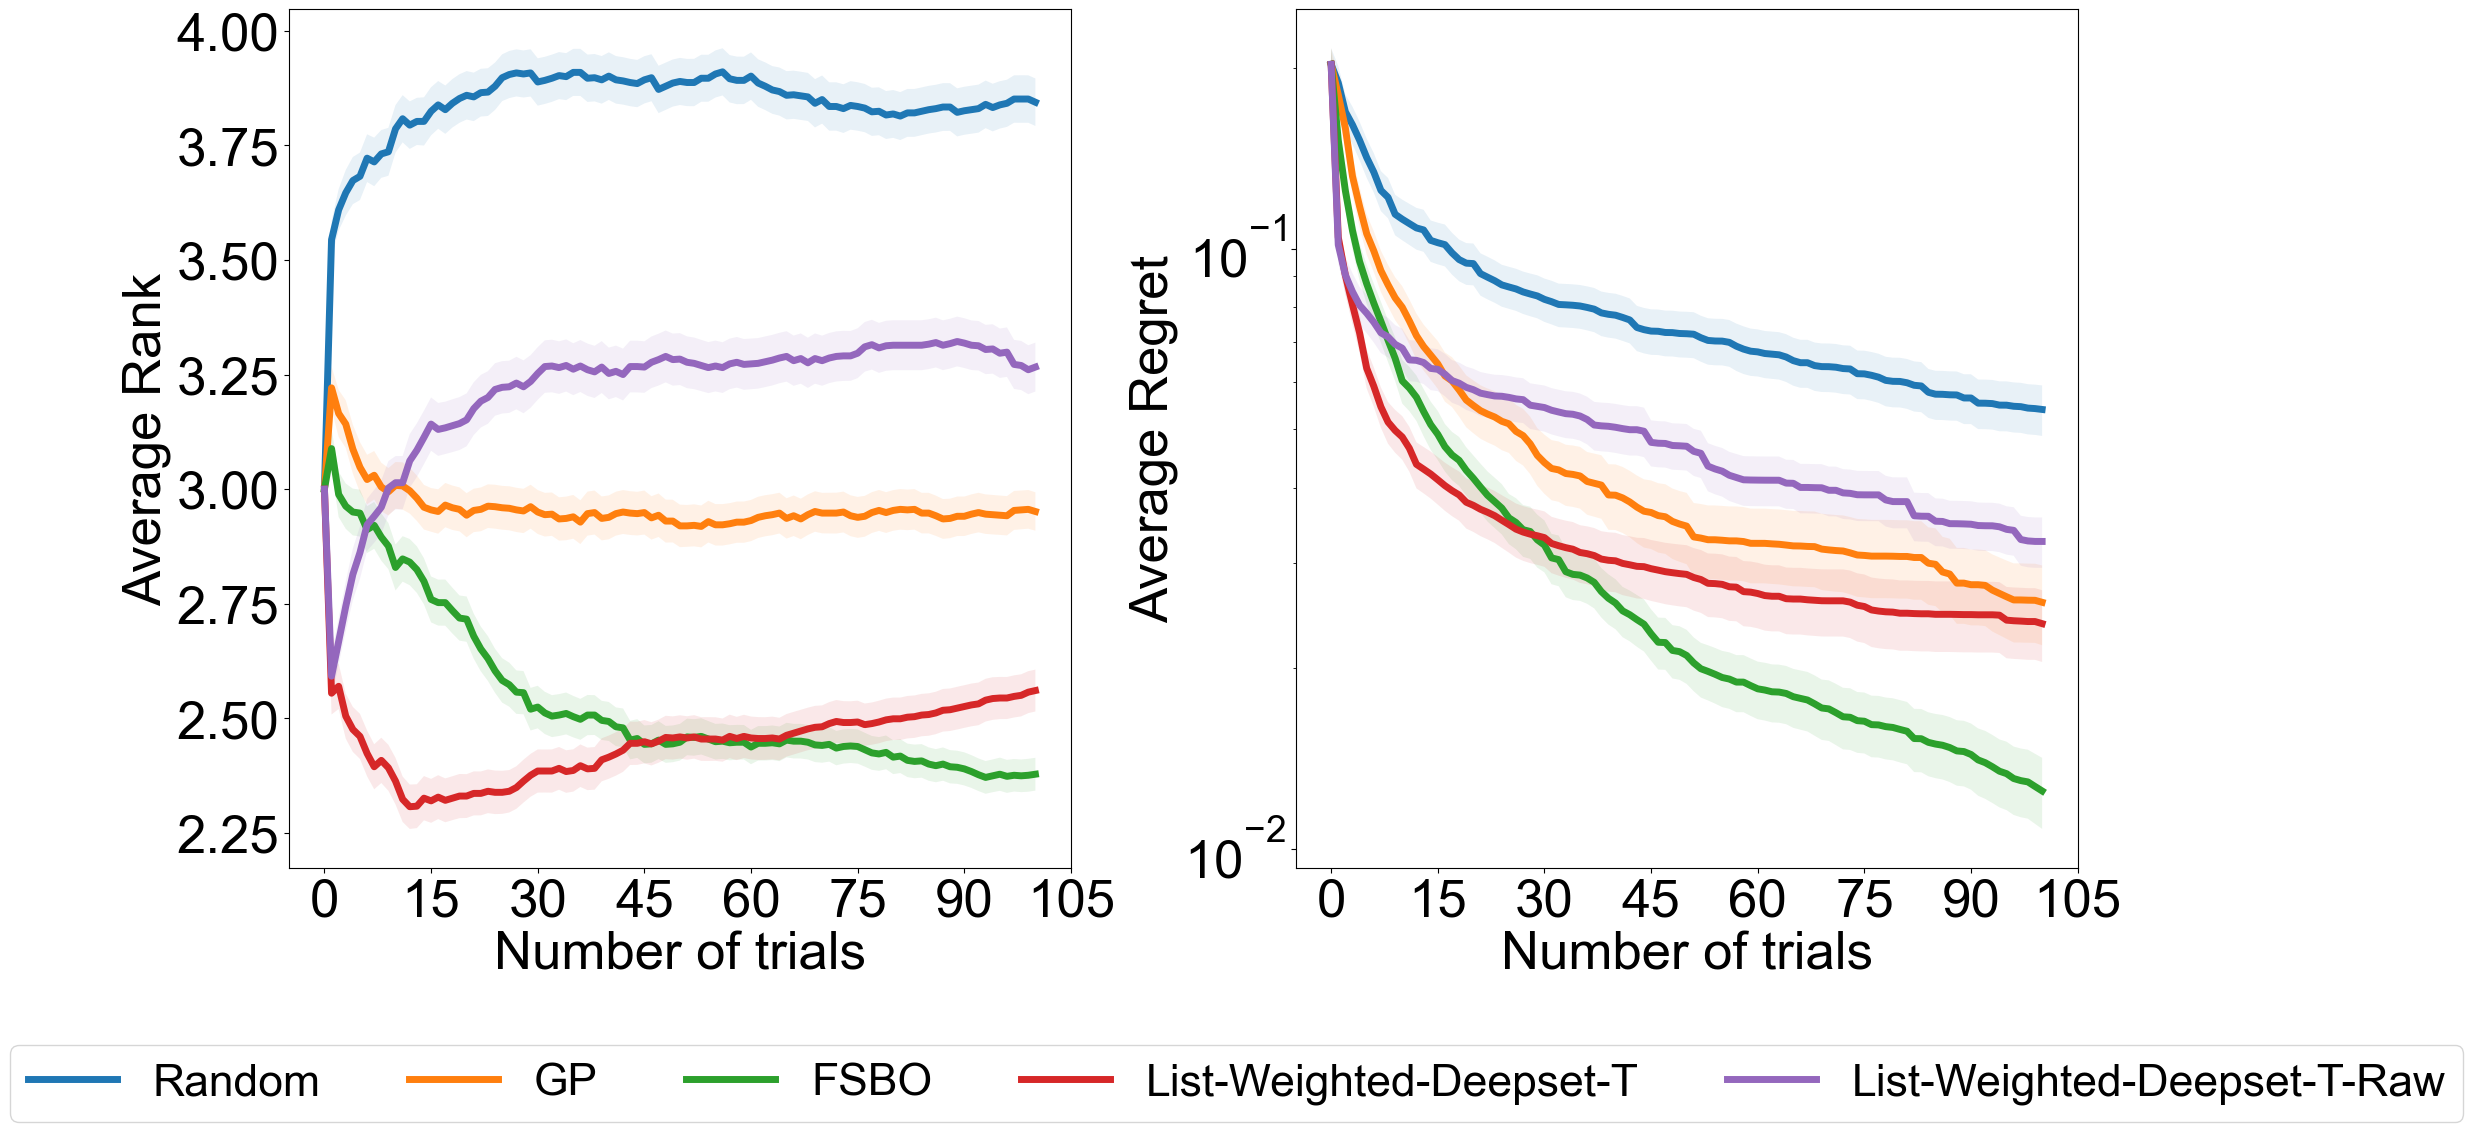
\includegraphics[scale=0.25]{images/FineTuningAblation}
    \caption{Studying how finetuning affects the optimization performance.}
    \label{fig:FineTuningAblation}
\end{figure}

From Figure~\ref{fig:FineTuningAblation} one can see that finetuning does help make the model get better results in the long run.
One fascinating result we see is that without any finetuning, the ranking loss surrogate shows good performance in the first evaluation steps.
This is because the surrogate model learns the best HP configuration found in the training metadata during meta-training.
Hence it selects these HP configurations in the first evaluation steps.
It makes intuitive sense because this behavior is shown by experts who try out the best HP configuration seen in their experience in the first evaluations. On average, this strategy works very well; hence the first evaluations were good for the non-finetuned surrogate model.
However, as the optimization steps proceed, the surrogate can condition its selection on more data. This conditioning is only done when the model is finetuned. Hence the finetuned surrogate works better in the long run.

\subsection{Comparing results with SOAT surrogates}
After analyzing our proposed model, one natural question is how it performs against the state-of-the-art HPO surrogates. We compare our results with the best-performing transfer and non-transfer HPO surrogates to answer this question.

Figure~\ref{fig:NonTransferSOAT} compares the results with some prominent state-of-the-art non-transfer HPO surrogates. We see from this figure that the proposed model far outperforms these surrogates. This is natural because our model is a transfer model and has the advantage of getting meta-trained before being used in the optimization.

Interestingly, the average regret of the proposed model at the end of optimizations is not very good compared to non-transfer surrogates.
Since the average regret gives a biased estimation of the results and the rank graph is a more accurate picture,  we conclude here that the proposed ranking loss surrogate model is better than the non-transfer surrogates.

\begin{figure}[h]
  \centering
    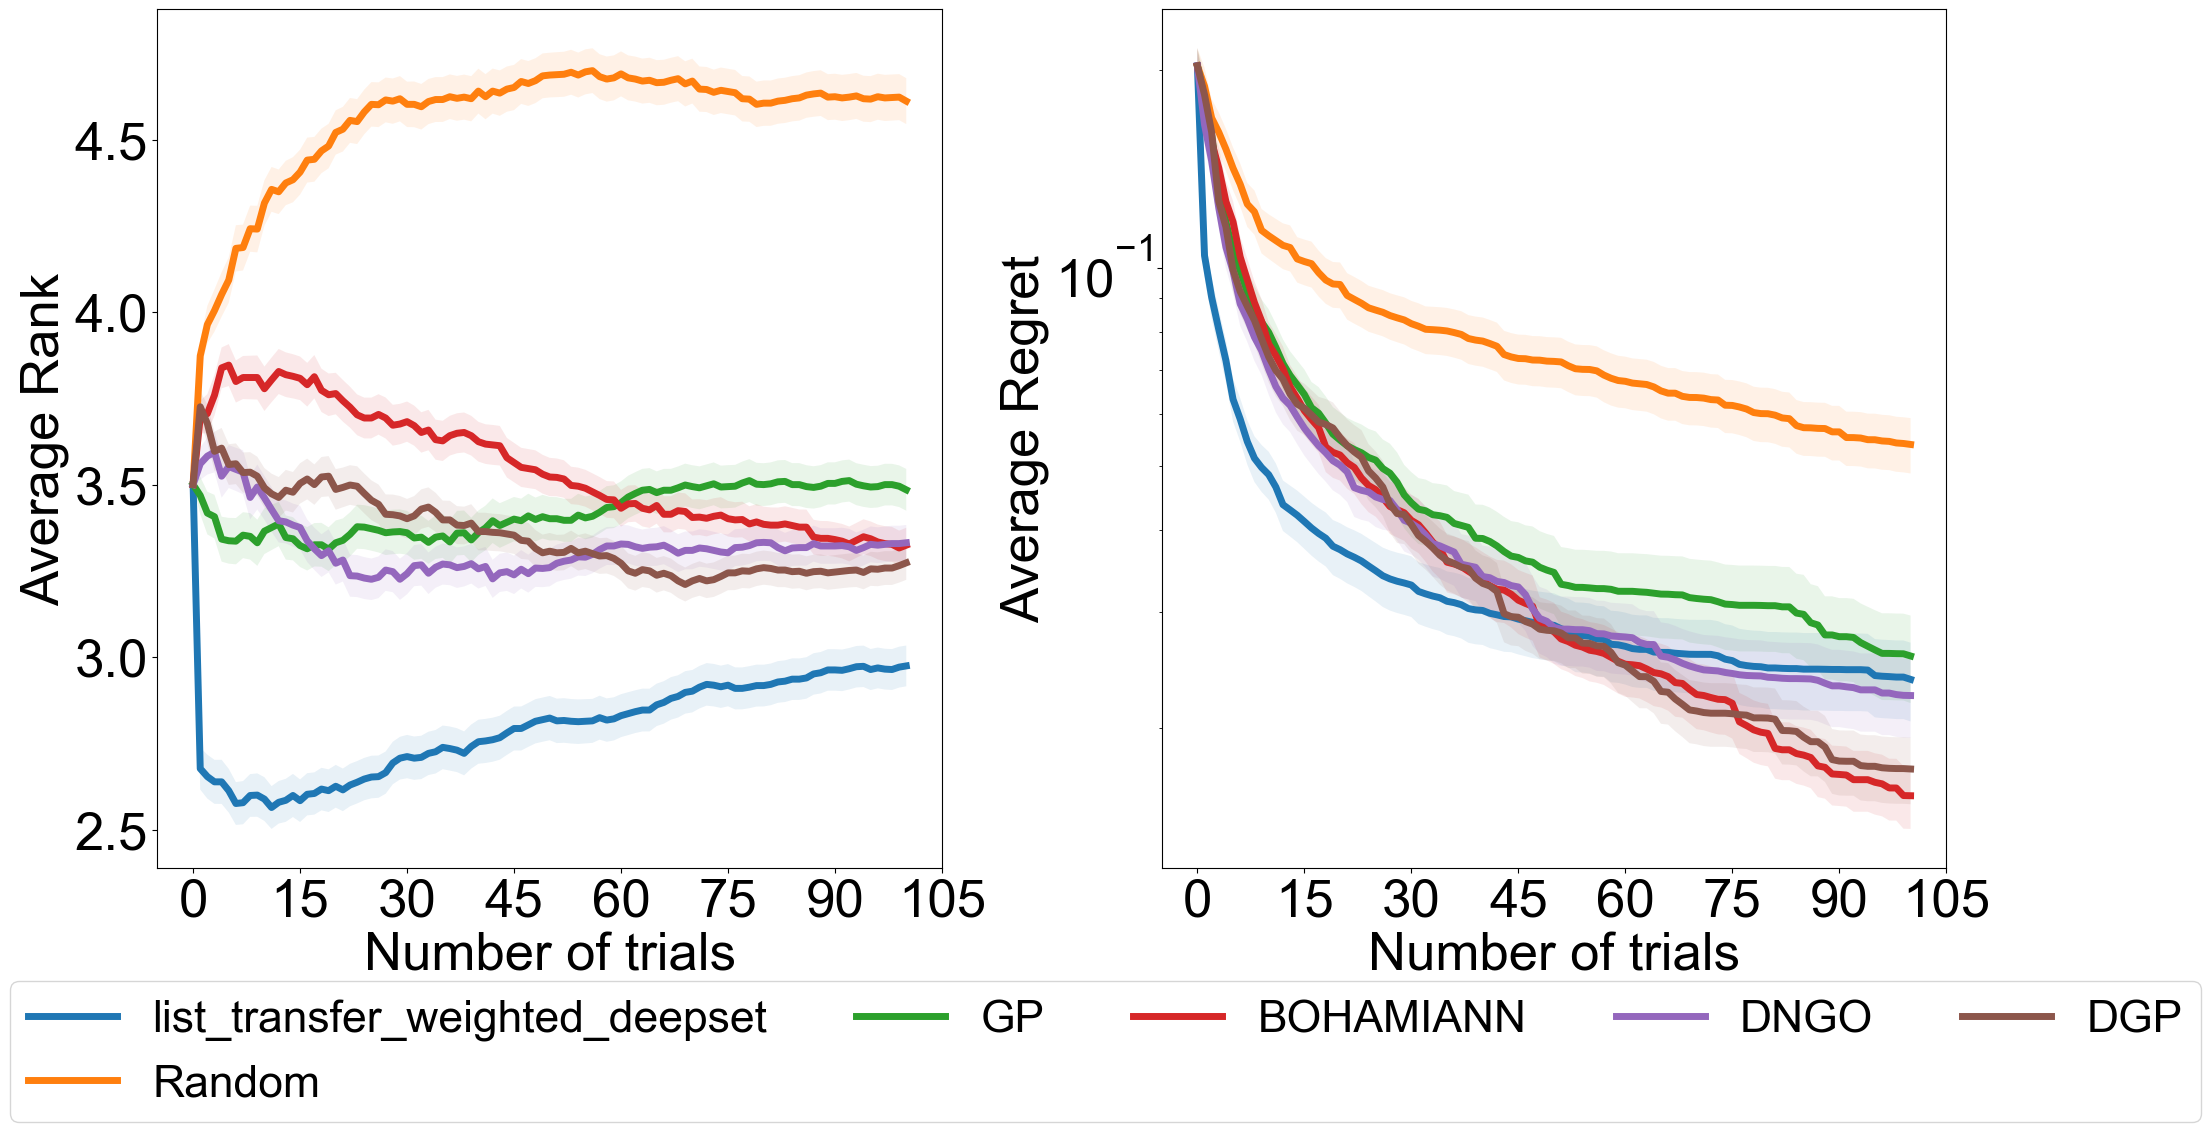
\includegraphics[scale=0.25]{images/NonTransferSOAT}
    \caption{Comparing our results against other non-transfer HPO surrogates.}
    \label{fig:NonTransferSOAT}
\end{figure}


Figure~\ref{fig:TransferSOAT} however, compares the results with other state-of-the-art transfer HPO surrogates. As we see from this figure, the strength of using the proposed model is that it outperforms the state-of-the-art results in the first evaluations in the optimization procedure. Moreover, it outperforms RGPE, which also uses the concept of ranking making our model unequivocally better performing than other ranking methods. This can also be seen in the critical rank graphs shown in Figure~\ref{fig:SOATCriticalRankedGraph}.

\begin{figure}[h]
  \centering
    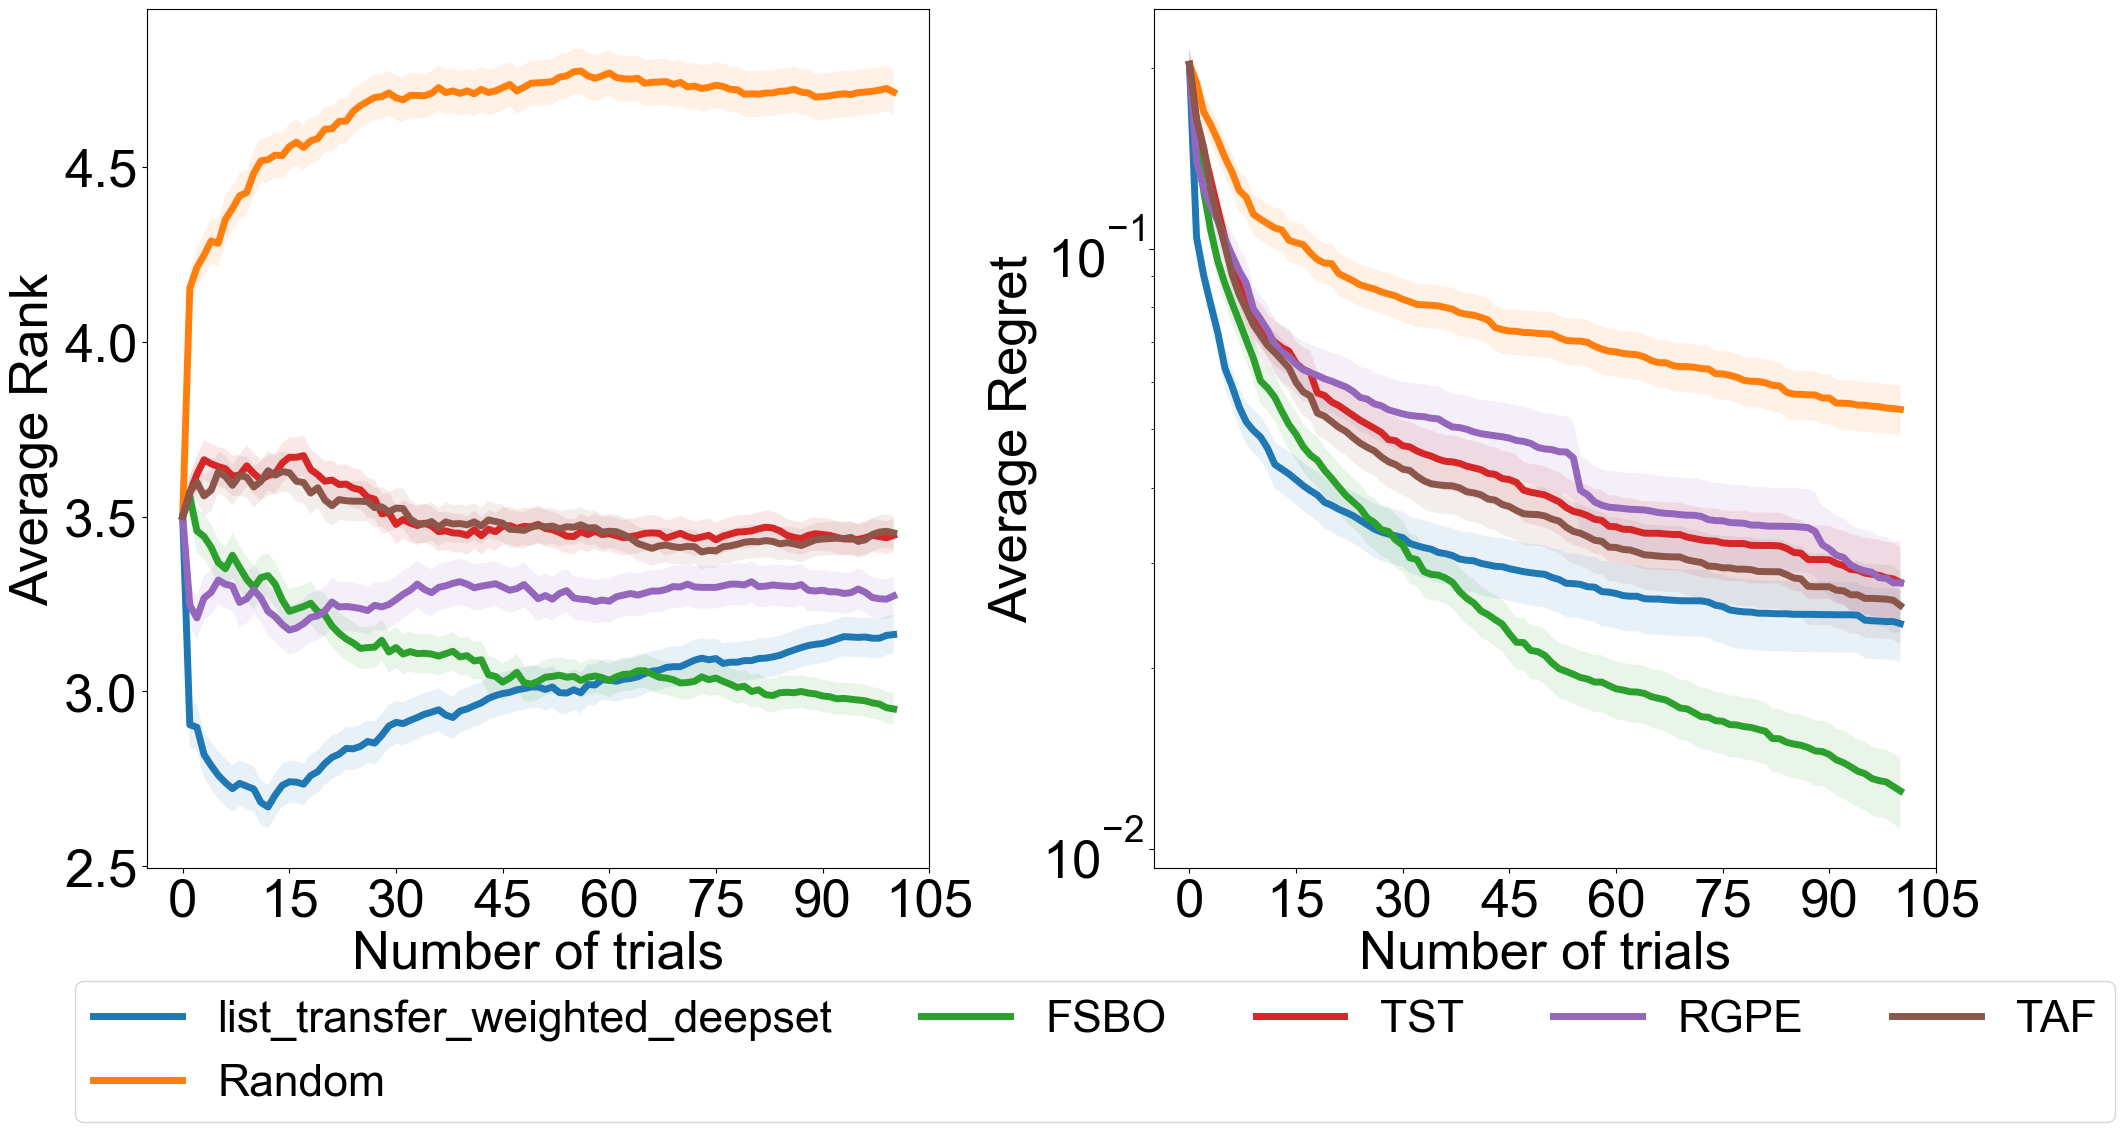
\includegraphics[scale=0.25]{images/TransferSOAT}
    \caption{Comparing our results against other transfer HPO surrogates.}
    \label{fig:TransferSOAT}
\end{figure}

\begin{figure}[h]% [H] is so declass\'e!
\centering
\begin{minipage}{0.45\textwidth}
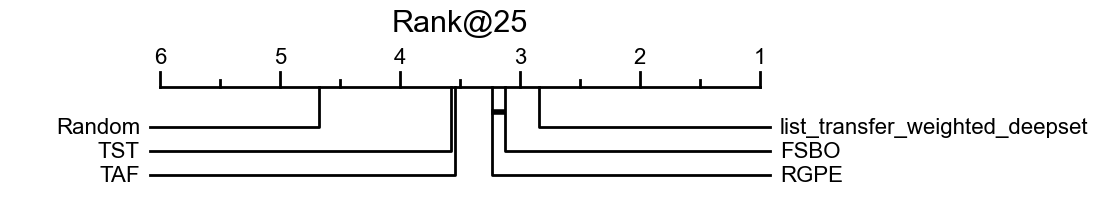
\includegraphics[width=\textwidth]{images/TransferSOATRank@25}
\end{minipage}\hfill
\begin{minipage}{0.45\textwidth}
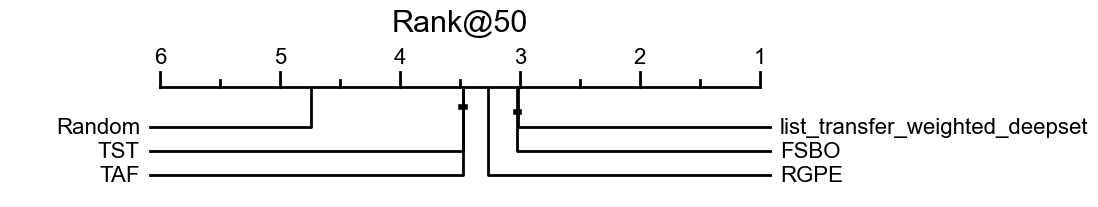
\includegraphics[width=\textwidth]{images/TransferSOATRank@50}
\end{minipage}\par
\vskip\floatsep% normal separation between figures
\includegraphics[width=0.45\textwidth]{images/TransferSOATRank@100}
    \caption{Critical rank graph the proposed model with other transfer HPO surrogates.}
   \label{fig:SOATCriticalRankedGraph}
\end{figure}

\subsection{Final ablation}
Finally, in this section, we show the ablation of all the different ranking loss surrogates that were used in the previous ablations. Figure~\ref{fig:FinalAblation} shows this ablation. In this figure, we can see that making the model a transfer model, weighting the ranking loss, and adding deep sets all significantly improved the proposed model's performance. 
The biggest strength of the proposed model is that it is excellent in the initial 30-40 steps of the optimization process (compared to state-of-the-art HPO surrogates). This is crucial for a sequential process like SMBO because selecting a good HP configuration in a particular step affects the selection of subsequent HP configurations.
The second strength of the model is that there is a possibility of reducing negative learning from occurring because of the context encoded using the deep sets.

\begin{figure}[h]
  \centering
    \includegraphics[scale=0.20]{images/FinalAblation}
    \caption{Ablation of all ranking loss surrogate models.}
    \label{fig:FinalAblation}
\end{figure}


\iffalse
Data used in the experiment
Infrastructure used
(That is the protocol)
Results should be structured like hypothesis.

experiment and results
protocol
data split…

First show the resutls of implementation of GP (M = 5 and M =10 )
Benchmark this...

Next with DKT (Benchmark this)

Next show the best results obtained by architecture.
\fi

\section{Advantages and Limitations}
\label{sec:advantagesAndLimitations}

In this section we first discuss some of the major advantages of the proposed model when compared to the baselines.
Then we move on to critically analyse the limitations of the model.

First and foremost,  one advantage of the proposed surrogate model is that it is a transfer HPO surrogate.  Previous available meta data will help the model to give better performance over non transfer HPO surrogate.

Secondly,  even if the amount of meta data is limited it has little affect on the training.
This is due to the nature of the loss function and the amount of data points that can be sampled during meta training.
For example,  if we have a meta data set of 100 observations i.e 100 ($X$,$y$) pairs,  and we have a list size of 15,  then the total number of training samples is given by $100C15$.
Hence the sampling method used gives us data that is exponential in number.
And each sampled list is a unique instance to train.
This is a big advantage for us as we can increase the complexity of the surrogate model with relative easy.
This also has a big advantage during fine tuning where the data is very less.

Another major advantage is that the range or the distribution of the actual scores is irrelevant for the training procedure.
This inherently dampens the effect of uncertainty by itself.
As the order of the known evaluations is the  only relevant thing,  minor variations in the output of the objective function has no effect on the training of the loss.
This also gives us flexibility of tampering the range of our surrogate based on our requirement.

\subsubsection{Disadvantages}
Our proposed model does have some limitations which need to be further studied.
Some of these are
\begin{itemize}
\item In our model,  a scorer is first learnt and then using this scorer,  we rank the set of query HP configurations.
During our training of the scoring model/surrogate,  we ignore the sorting functionality necessary to complete the process of ranking.
This is because sorting is non differentiable. 
Which means that the true evaluation of the ranked list is not optimized.

\item Our loss function makes use of exponentiation function as the strictly increasing positive function.
This puts a major restriction on the range of the relevance scores.
It may not have the output space to completely map the range of the true scoring function.
More research is required to find out better strictly increasing functions.

\item The range controller function we use in our model is $\tanh$ because of the function's smoothness.
However,  if the output relevance scores of 2 HP configurations are either at the positive extreme or negative extreme,  then it may be difficult to distinguish between them.
This can be dampenned by tuning the $k$ and $\alpha$ parameters as discussed in Section~\ref{sec:BasicScoringModelDNN},  but this does have practical limits due to the floating point implementations in computer languages.

\item It is during the meta training that all the meta training tasks / meta datasets have the same output range for simplicity.
This is the case of all outputs HPO-B.
If there is any other meta data used,  the outputs of the different meta data (tasks) should be normalized before being used in the training process.

\item The meta trained model may be biased towards one task due to a larger availability of data from this task.
This is however dampened by the fact the we are using the double sampling mechanism.
This makes sure all the tasks sampled equal number of times.
However,  this leads to over fitting of the model towards the tasks that have lesser data because this data is overused during training.

\iffalse
\item The quality requirement of the uncertainty estimation and need for it is not always the same.
The search spaces that have less data need more uncertainty and vis versa.
 The learnt model is extremely sensitive to the learning rate and the number of epochs.
\fi

\end{itemize}
    
\subsubsection{Negative transfer learning}
\label{sec:NegativeTransferLearning}
For some search spaces,  the validation errors of the ranking loss model did not reduce at all during its training.
In fact the validation loss became worse.
Figure~\ref{fig:NegativeLearning} shows an illustration of this for the search space id 5527.
This is a classic example of negative transfer learning~\cite{Weiss2016}.
Negative transfer learning occurs when the set of source tasks (here,  training datasets) is very different from the target tasks (here, validation datasets).

\begin{figure}[htb]
  \centering
    \includegraphics[scale=0.5]{images/NegativeLearning}
    \caption{Training loss curve of ranking losses}
    \label{fig:NegativeLearning}
\end{figure}

This problem should occur only in the cases where the model is context free.
In our case,  the ranking loss model with deep set is context aware and results like these were unexpected.
Hence the issues with negative transfer learning remains unsolved when using our model.
One remedy for getting around this problem is to fine tune the model with a larger number of epochs.
Nevertheless,  we cannot guarantee that the fine tuning will re-learn from the small amount observed data points during the optimization cycle.
Note: Since the testing/evaluation task may be similar to the training task,  we did not do any early stopping.

\iffalse
\section{Evaluation}
\subsection{Testing}
explain how a ranking graph works ar implemented
Explain the regret rank@ some location.

\subsection{Ablation}

Result tabulation of case study: sorting:
1.  Within range
2.   Outside range 
mean of 3 times should be written.

show the results of raw without deep set.

Next show different strategies used for building the ranking loss model one step at a time.
First with only scorer.
then with deep set.
Then with raw deep set
fine tuning and deep set
adding uncertainty

Checking the early stop and hypothesing why is was wrong.

box plot variation of each of the scorers... for 1 or more data sets?

show results of independent training and training with output restriction

what about training independently,   this requires normalization. 
as explained by sebastian.
\fi

\chapter{Conclusion}

The ranking loss surrogate model proposed in this thesis has a few limitations and gaps which need to be researched and implemented. 
As the scope of this thesis was limited we could not explore many research directions.
In this section we mention some of the topics that could be interesting to take up in any further research in this area.
Thereafter we conclude our thesis.

\section{Further research work}

We introduced uncertainty into our model with the use of Deep Ensembles. 
With this we had many basic scoring models each giving their own.
The mean of these neural networks was taken to be the joint output of the
ensemble.
This mean was used by the loss function to train the whole model.
We can term this as "collective training" of the ensemble.
There is,  however,  also the possibility of independent training where each neural network is trained independently.
Some intricacies if we train this way are
\begin{itemize}
\item The Deep Set architecture is a backbone that is common to all basic scoring models.  How is this to be trained?
\item Independent training implies that the range of the output of different basic scoring models is different. 
Are these to be normalized? Or do we take the ranking from all scoring models and average them.
\end{itemize}

In the proposed model,  the deep neural networks output a list of output scores. 
We use this output to calculate the mean and the variance of the scores.
The deep ensemble, however, paper proposes a method to directly calculate the mean and this variance.
The integration of this idea with ranking losses is non-trivial.
Hence the integration of this Deep Ensemble architecture with the ranking loss function can be taken up in further research work.
It would be interesting to see the affect of this integration for HPO problems with very less meta data because Deep Ensembles by themselves as introduced by ~\cite{DeepEnsemblePaper} perform relatively good in the evaluation phase.

This thesis has primarily focused on how to select HP configurations from a set of discrete HP configurations.
Hence the model does not deal with continuous search spaces directly.
For working with continuous HP search spaces,  we can divide the space  (in the euclidean sense) into hyper-volumes and use 1 HP configuration as a representative for the whole hyper-volume.
Then we may select the best region and subdivide the space and continue the process till a particular granularity.
This method is just a workaround to the main problem and we also cannot really guarantee that an optima will be found in contract to any gradient based optimization method.
Hence,  further research needs to be done on how to formulate the ranking loss function for continuous search spaces.

We already discussed in Section~\ref{sec:advantagesAndLimitations}  that the ranking loss function does not optimize the sorting function.
The inclusion of sorting functionality in the loss function has  been proposed and studied in Swezey et.  al~\cite{PiRank}.
On research direction would be to incorporate the ideas of PiRank in order to see if there is any improvement in the model.

Lastly,  novel HPO surrogates that have not been explored by this thesis can be implemented.
This would not only further the research empirically but also ideas used in other baselines could be incorporated to improve the model.


\section{Conclusion}
In this thesis we study a method of Hyper parameter optimization using Sequential Model based Optimization algorithm as a reference algorithm.
The angle of approach to this problem however is different from usually studied HPO methods.
We formulated the problem of selecting next HP configurations within the SMBO cycle as a problem of ranking.
Due to the nature of the ranking losses studied by us,  we needed to design a suitable surrogate for it.

In the quest to design get good performance for our proposed model we systematically studied and chronologically added essential components to the model which were - addition of context using deep sets,  addition of weighting to the loss function and the addition of uncertainty to the model.
We found that the model with all the these components gave results which were on par with the state of the art results of FSBO.
The reason for this,  we hypothesis, is that the training and sampling mechanism for the loss function is very different as compared to the other HPO surrogates or losses.
The advantage that our model is able to sample combinatorial number of samples from a given set of HP configurations is a upper hand for the proposed model.

Even though we cannot claim the superiority of this method unequivocally due to the scope of application of the ranking loss functions,  we do encourage the reader to pursue further research in this area. 
We believe from our research the models trained using ranking losses have the potential to give very good Hyper parameter optimization results.
We also believe that the concepts developed in this thesis could aid in other areas of research like Information retrieval which heavily use ranking losses.





\iffalse
\subsubsection{Training with mean and restricted output}
Implementation yet to be done
\fi

\iffalse
Paper: https://arxiv.org/pdf/2012.06731.pdf
       (Impt Ref) https://arxiv.org/pdf/1903.08850.pdf

Key Idea:
    Use permutation matrices to represent sorting. Learn the matrix with the loss function.
    [0 1 0] [x]    [y]
    |1 0 0| |y|  = |x|
    [0 0 1] [z]    [z]
    Permutation Matrices are not smooth in the input space Hence relaxation is necessary for differentiability
    Relaxation is done by using a double schocastic matrices i.e all row and column matrices sum to 1.

    Unimodal
    Double schochastic

The idea of Permutation Matrices is taken from Neural sort - Neural sort (Impt ref)

PLACKETT-LUCE DISTRIBUTIONS -> Very important to explain the rationale about using score as a probability
    measure for our scoring function (Check section 2.1 of paper 2 (Neural Sort))
\fi 


\bibliography{references}
\bibliographystyle{plain}


\appendix
\pagenumbering{roman}
\chapter{Controlling the output range}
\label{chap:OutputRangeControl}

Lets take the listwise loss function $L_{mle}$ which is nothing but maximum log-likelihood estimation. 
In our surrogate models, we use the strictly positive increasing function $\exp$ as proposed by Fen et. al.~\cite{listmlepaper}.
Hence, our $L_{mle}$ becomes 
\begin{equation}\label{eq:overflowissue}
L_{mle} = -  \sum\limits_{j=1}^{k} \log \frac{\exp(s(\pi^*_j))}{ \sum\limits_{t=j}^k \exp(s(\pi^*_k))}
\end{equation}

Even though theoretically, the score range does not need to be restricted, we have practical limitations due to implementation constraints of floating-point numbers.
Due to the exponentiation in our loss function, if the score range is too high,  the values in equation~\ref{eq:overflowissue} may overflow.
On the other hand, if it is too small, the values may underflow.
In both these cases, we are bound to get NAN (Not A Number) exceptions when executing our implementations.
We would also get similar issues for the pair-wise loss function because we use exponentiation for calculating the probability, as shown in equation~\ref{eq:pairwiseprobability}.
One way to eliminate this issue is to use the log-sum-exp trick. This trick is used in the ListMLE implementation given by Pobrotyn
 et. al. ~\cite{Pobrotyn2020ContextAwareLT} and we use this implementation in our thesis.

However, if the output score is used anywhere other than ranking, we would need to control its range.
We can do this by passing the output of the deep neural network through a $\tanh$ function.
If we would like to strictly limit the range of our function between $[-k,  k]$,  then we can pass the output score through the following function
\begin{equation}\label{eq:tanhEquation}
k * \tanh(\alpha * s(\textbf{X}))
\end{equation}

Here $\alpha$ is the smoothness factor which is inversely proportional to the smoothness of the $\tanh$ graph~\cite{tanhstackoverflowanswer}.
Figure~\ref{fig:tanhGraph} shows how to vary the smoothness and range of the output using $\alpha$ and $k$ respectively.
\iffalse
We used $k=2$ and $\alpha=0.01$ for our scorer.
\fi

\begin{figure}[htb]
  \centering
    \includegraphics[scale=0.5]{images/tanhGraph}
    \caption{Effect of varying $k$ and $\alpha$ in equation~\ref{eq:tanhEquation}.}
    \label{fig:tanhGraph}
\end{figure}


\iffalse
% \chapter*{Appendices}
\chapter{More information}
This thesis was completed in the representation learning lab of Albert-Ludwig-Universität Freiburg.  (Figure~\ref{fig:UniLogo})


\begin{figure}[htb]
  \centering
    \includegraphics[scale=0.35]{images/logo}
    \caption{Logo: Albert-Ludwig-Universität Freiburg}
    \label{fig:UniLogo}
\end{figure}

\fi

\end{document}